%for a more compact document, add the option openany to avoid
%starting all chapters on odd numbered pages
\documentclass[11pt]{cmuthesis}

% This is a template for a CMU thesis.  It is 18 pages without any content :-)
% The source for this is pulled from a variety of sources and people.
% Here's a partial list of people who may or may have not contributed:
%
%        bnoble   = Brian Noble
%        caruana  = Rich Caruana
%        colohan  = Chris Colohan
%        jab      = Justin Boyan
%        josullvn = Joseph O'Sullivan
%        jrs      = Jonathan Shewchuk
%        kosak    = Corey Kosak
%        mjz      = Matt Zekauskas (mattz@cs)
%        pdinda   = Peter Dinda
%        pfr      = Patrick Riley
%        dkoes = David Koes (me)

% My main contribution is putting everything into a single class files and small
% template since I prefer this to some complicated sprawling directory tree with
% makefiles.

% some useful packages
\usepackage{times}
\usepackage{fullpage}
\usepackage{graphicx}
\usepackage{amsmath}
\usepackage{amssymb}
\usepackage[numbers,sort]{natbib}
\usepackage[backref,pageanchor=true,plainpages=false, pdfpagelabels, bookmarks,bookmarksnumbered,
%pdfborder=0 0 0,  %removes outlines around hyper links in online display
]{hyperref}
\usepackage{subfigure}
\newtheorem{theorem}{Theorem}[section]
\newtheorem{corollary}{Corollary}[theorem]
\newtheorem{lemma}{Lemma}[theorem]
\newtheorem{definition}{Definition}
\newtheorem{proposition}{Proposition}
\newenvironment{proof}{\paragraph{Proof:}}{\hfill$\square$}
\newcommand{\theHalgorithm}{\arabic{algorithm}}

% Approximately 1" margins, more space on binding side
%\usepackage[letterpaper,twoside,vscale=.8,hscale=.75,nomarginpar]{geometry}
%for general printing (not binding)
\usepackage[letterpaper,twoside,vscale=.8,hscale=.75,nomarginpar,hmarginratio=1:1]{geometry}

% Provides a draft mark at the top of the document. 
% \draftstamp{\today}{DRAFT}

\usepackage{tikz}
\usetikzlibrary{
  arrows.meta, % for Straight Barb arrow tip
  fit, % to fit the group box around the central neurons
  positioning, % for relative positioning of the neurons
  bayesnet
}

\DeclareMathOperator{\argmax}{\arg\max}
\DeclareMathOperator{\argmin}{\arg\min}

\DeclareMathOperator*{\minimize}{\text{minimize}}
\DeclareMathOperator*{\maximize}{\text{maximize}}
\DeclareMathOperator*{\st}{\text{subject to}}
\usepackage{tabularx,booktabs}
\def\usevspace{1}

\usepackage{algorithm}
\usepackage[noend]{algorithmic}
\usepackage[algo2e,linesnumbered,vlined,ruled]{algorithm2e}
\usepackage{multirow}
\usepackage{centernot}
\tikzset{
  neuron/.style={ % style for each neuron
    circle,draw,thick, % drawn as a thick circle
    inner sep=0pt, % no built-in padding between the text and the circle shape
    minimum size=3em, % make each neuron the same size regardless of the text inside
    node distance=1ex and 2em, % spacing between neurons (y and x)
  },
  group/.style={ % style for the groups of neurons
    rectangle,draw,thick, % drawn as a thick rectangle
    inner sep=7pt, % no padding between the node contents and the rectangle shape
  },
  group2/.style={ % style for the groups of neurons
    rectangle,draw,thick, % drawn as a thick rectangle
    inner sep=7pt, % no padding between the node contents and the rectangle shape
  },
  io/.style={ % style for the inputs/outputs
    neuron, % inherit the neuron style
    fill=gray!15, % add a fill color
  },
  conn/.style={ % style for the connections
    -{Straight Barb[angle=60:2pt 3]}, % simple barbed arrow tip
    thick, % draw in a thick weight to match other drawing elements
  },
}

\begin {document} 
\frontmatter

%initialize page style, so contents come out right (see bot) -mjz
\pagestyle{empty}

\title{ {\it \huge Thesis Proposal}\\
{\bf Practical Methods for Automated Algorithm Design \\ in Machine Learning and Computational Biology}}
\author{Minh Hoang}
\date{May 2022}
\Year{2022}
\trnumber{}

\committee{
Prof. Carl Kingsford, Chair \\
Prof. David P. Woodruff \\
Prof. Maria-Florina Balcan \\
Prof. Risto Miikkulainen
}

% \support{}
% \disclaimer{}

% copyright notice generated automatically from Year and author.
% permission added if \permission{} given.

\maketitle

% \begin{dedication}
% For my dog
% \end{dedication}

\pagestyle{plain} % for toc, was empty

%% Obviously, it's probably a good idea to break the various sections of your thesis
%% into different files and input them into this file...
\begin{abstract}
Configuration tuning is often a key element in achieving outstanding performance with parameterized algorithmic solutions. However, it often requires extensive manual effort to satisfactorily configure an algorithm for a specific task instance, thus preventing these algorithms to be deployed at scale. More importantly, without a principled method to configure these deployment settings, it will be difficult to reproduce the obtained results under other experimental conditions. To address these problems, this thesis focuses on developing novel automated algorithm design (AAD) frameworks capable of configuring algorithms for specific use cases in a data-driven manner. Particularly, we cast these AAD problems as optimization tasks that aim to maximize some performance metric with respect to the configurations of the solution model. We ground our investigation in three specific classes of AAD problems, including kernel selection for Bayesian inference, architecture search for deep neural network and minimizer construction for sequence sketching. In all of these problems, the variables to be optimized often have underlying discrete structures such as trees, graphs or permutations. Our contribution is a suite of reformulation techniques that result in efficient and accurate tuning methods for these configuration domains. Finally, we demonstrate the performance of our methods on practical scenarios and show that they have significantly outperformed state-of-the-art benchmarks.
\end{abstract}
\keywords{Automated Machine Learning, Optimization}
% \begin{acknowledgments}
% \input{acknowledgement.tex}
% \end{acknowledgments}



\tableofcontents
\listoffigures
\listoftables

\mainmatter

%% Double space document for easy review:
\renewcommand{\baselinestretch}{1.66}\normalsize

% The other requirements Catherine has:
%
%  - avoid large margins.  She wants the thesis to use fewer pages, 
%    especially if it requires colour printing.
%
%  - The thesis should be formatted for double-sided printing.  This
%    means that all chapters, acknowledgements, table of contents, etc.
%    should start on odd numbered (right facing) pages.
%
%  - You need to use the department standard tech report title page.  I
%    have tried to ensure that the title page here conforms to this
%    standard.
%
%  - Use a nice serif font, such as Times Roman.  Sans serif looks bad.
%
% Other than that, just make it look good...


\chapter{Introduction}
\label{c1:intro}
\section{Automated Algorithm Design}
A vast majority of algorithms are typically developed with parameters that can be configured by users depending on their use cases. Although it is convenient to use a default configuration for every application, such a tactic is often sub-optimal when performance is sensitive to the choice of configurations\cite{balcan2021much,thornton2013auto}. In Bayesian statistics, choosing an appropriate kernel function to model data correlation can strongly influence the outcome of probabilistic inference \cite{Duvenaud13}. In deep learning, the design of a neural network architecture (e.g., the number of layers, types of activation functions and number of neurons in each layer) must be carefully selected to achieve optimal performance on specific scenarios \cite{pham2018,he2020fednas,zoph2016}. For example, convolutional neural network architectures that excel on computer vision tasks \cite{lecun2015lenet,he2016deep} might under-perform in language processing problems, which have been found to favor attention-based modelling \cite{vaswani2017attention}. 

Due to this inconsistent behavior, a more practical approach is therefore to calibrate the design of an algorithm on a \emph{per-task} basis, which seeks to find the most suitable model configuration for each new problem instance. Despite the potential improvements that optimally configuring an algorithm can have on its performance, this calibration step is traditionally driven by domain expert experience and manual heuristics, and hence inefficient and difficult to scale or reproduce. This absence of a principled approach for configuring algorithmic solutions has motivated the study of automated algorithm design (AAD) through systematic optimization frameworks, which was first considered in the seminal work of \citet{rice1976algorithm} and subsequently in various algorithmic domains such as deep learning \cite{pham2018,he2020fednas,Idrissi16}, non-parametric Bayesian methods \cite{Duvenaud13,Malkomes16,Lu18} and discrete algorithms \cite{zheng20miniception,zheng21}. Formally, the general AAD problem is described as follows:

\begin{definition}[Automated Algorithm Design]
Let $\mathcal{T}$ be an arbitrary space of computational tasks and $\mathcal{M}$ be a likely infinite set of algorithms capable of solving any task $\tau \in \mathcal{T}$. Given a performance evaluation function $F: \mathcal{T} \times\mathcal{M} \rightarrow \mathbb{R}$, we say that an algorithm $m \in \mathcal{M}$ outperforms $m' \in \mathcal{M}$ on some task $\tau \in \mathcal{T}$ if and only if $F(\tau, m) > F(\tau, m')$. Then, for any task $\tau \in \mathcal{T}$, the AAD problem can be written as the following optimization task, which seeks to find the optimal algorithm $m_\ast \in \mathcal{M}$ such that $F(\tau, m')$ is maximized:
\begin{eqnarray}
m_\ast &\in& \underset{m \in \mathcal{M}}{\mathrm{argmax}} \ F(\tau, m) \ .
\label{aad-problem}
\end{eqnarray}
\end{definition}
\section{Related Work}
Due to the general nature of the performance measuring function $F$, the AAD task in Eq.~\eqref{aad-problem} is commonly viewed as a black-box optimization (BBO) problem, where $F$ is taken for an oracle that can be queried at will given some input configuration. Most existing black-box optimization methods tend to approach this task via a sequential optimization strategy which alternates between evaluating observations and making informed decision about subsequent probings of the oracle. Typically, this decision is either guided by practical heuristics or a surrogate model that estimates the relationship between configurations and evaluated performances. We summarize a few typical BBO methods below:

\subsubsection{Heuristic search}
One of the most classical approach to optimize this black-box function is grid search, which systematically evaluates all input configurations projected on a lattice to find the best performing candidate. For continuous configurations, this lattice is obtained by discretizing the search space, whereas for categorical configurations, this routine simply means exhaustively trying all combinations of values in each dimension. Alternatively, another widely-used approach for black-box optimization is random search, where inputs are chosen completely at random to evaluate. Both grid search and random search are straight-forward to implement and have been used in several AAD tasks \cite{bergstra2011algorithms,liashchynskyi2019grid,bergstra2012random}. These methods, however, only focus on exploring the search space and have no built-in mechanism to exploit the collected observations, thus tend to scale poorly with the complexity of the input domain. 

In contrast, other heuristic optimization methods such as coordinate ascent~\cite{friedman2010regularization,wright2015coordinate} and simulated annealing~\cite{bertsimas1993simulated} focus on refining the best candidate found so far in a greedy manner. Coordinate ascent achieves this by successively optimizing along a specific dimension while fixing every other dimension of the parameter space, repeating for all dimensions until convergence. Instead of making queries along a single coordinate, the simulated annealing algorithm alternatively evaluates a small neighborhood around the current best estimate and tries to move in the direction that yield the best improvement. Both methods have also been used in many AAD tasks~\cite{bergstra2011algorithms,bellio2016feature,deblasio2020more}, but are typically vulnerable to being trapped in local optima due to a lack of exploration mechanism.

\subsubsection{Evolutionary strategies}
Evolutionary strategies (ES) are optimization techniques inspired by nature, in which a population of configurations is set to evolve over time and improve its averaged performance while doing so. For every generation of this population, most evolutionary algorithms will conduct the following three steps: (1)~estimate the fitness of each individual in the population; (2)~generate new individuals using certain reproduction and/or mutation operators; and (3)~replacing unfit individuals with new individuals. 

Evolutionary algorithms~\cite{fogel1994introduction,banzhaf1998genetic} have been widely applied in automated algorithm design, such as model selection for deep neural networks~\cite{olson2016tpot,lorenzo2017particle,miikkulainen2019evolving,liang2019evolutionary} and support vector machines (SVM)~\cite{lin2008particle}; or finding clinical interventions~\cite{miikkulainen2021prediction}. These techniques fundamentally differ from the above heuristic algorithms by balancing between exploration and exploitation. For example, in genetic optimization, high-fitness individuals can partially pass down their representations to the next generation via a crossover operator (i.e., exploitation), in hope that good performances can be preserved and improved. At the same time, new representations are continually generated via the random mutation operator (i.e., exploration), thus ensuring the optimization is not trapped in local optima.

\subsubsection{Sequential model-based optimization}
Unlike the above methods which are considered model-free, sequential model-based optimization (SMBO) is an optimization paradigm which iteratively uses collected information to estimate a surrogate model for the black-box function $F$. This model is then used to guide the acquisition of subsequent observations. Different SMBO methods have been used to address various AAD tasks such as configuring parameterized tree search algorithms and local SAT solvers~\cite{hutter2011sequential}. We now give a description of the Bayesian optimization (BO) algorithm~\cite{Snoek12}, which is a widely-used variant of SMBO.

The general BO algorithm usually prescribes a Gaussian Process (GP) prior~\cite{Rasmussen06} over the black-box objective function, i.e. $F \sim \mathcal{GP}(\mu, k)$ where $\mu: \mathcal{M} \rightarrow \mathbb{R}$ and $k: \mathcal{M}\times\mathcal{M} \rightarrow \mathbb{R}$ are respectively the prior GP mean and covariance functions. This prior implies that for any finite subset of candidate configurations $\{m_1, m_2 \dots m_T\}$ the corresponding performance vector $\left[F(m_1) F(m_2) \dots F(m_T)\right]$ is normally distributed \emph{a priori} with mean $\left[\mu(m_1), \mu(m_2), \dots ,\mu(m_T)\right]$ and covariance $\left[k(m_i, m_j)\right]_{i,j\in[T]}$. At any iteration $t$, the BO algorithm then uses this prior distribution and the set $\mathcal{D}_t$ of collected observations so far to derive a posterior predictive distribution $p(F(m_\ast) \mid m_\ast, \mathcal{D}_{t})$ for any subsequent candidate $m_\ast$. 

The posterior predictive mean can be used directly to estimate the expected performance of subsequent candidates, thus allowing us to exploit high-performing configurations without actually evaluating $F$. However, since the posterior naturally has high uncertainty in unobserved regions, doing so would discourage thorough exploration of the search space and risk missing out on good solutions. To address this issue, the BO algorithm instead constructs an \emph{acquisition function} that incorporates both the posterior mean and covariance to balance this exploitation and exploration trade-off. For example, the upper confidence bound (UCB) acquisition function proposed by \citet{Srinivas10} is given by:
\begin{eqnarray}
\alpha_{\textsc{UCB}}(m; M_t, \sigma_t) &\triangleq& M_t(m) + \beta \sqrt{\sigma_t(m)} \ ,
\end{eqnarray}
where $M_t(m)$ and $\sigma_t(m)$ respectively denote the posterior mean and variance at iteration $t$ given some candidate $m$. Here, the parameter $\beta$ reflects the trade-off between exploiting candidates with high expected performance and exploring candidates with high uncertainty. Finally, the BO algorithm can be described via the following update rules:
\begin{eqnarray}
m_{t+1} &=& \underset{m \in \mathcal{M}}{\argmax} \ \alpha_{\textsc{UCB}}\left(m; M_t, \sigma_t\right) \ , \nonumber \\
\mathcal{D}_{t+1} &=& \mathcal{D}_{t} \cup \{(m_{t+1}, F(m_{t+1})\} \ , \nonumber \\
M_{t+1}, \sigma_{t+1} &\leftarrow& p\left(F(m_\ast) \mid m_\ast, \mathcal{D}_{t+1}\right) \ .
\end{eqnarray}
Nonetheless, we remark that the vanilla BO algorithm is best suited for low-dimensional and continuous input domains. In practical AAD tasks where the space of configuration is structured and discrete, there is generally no unifying approach to parameterize the mean and covariance function of the GP surrogate. Furthermore, optimizing the acquisition functions will also become non-trivial and require special modelling considerations. 

\subsubsection{Domain-specific AAD approaches}
In many specific AAD problems, $\mathcal{M}$ can be specified as a sub-class of algorithms that is described by discrete data structures such as sub-trees \cite{Duvenaud13}, graphs \cite{he2020fednas, pham2018, bender2018understanding} or permutations \cite{marcais17}. This choice of representation implicitly prescribes a correlation structure among candidate models via the topology of $\mathcal{M}$ and thus allows the general AAD objective to subsequently be cast as optimization/search tasks on these structured domains. 

This thesis will focus on three such prototypical classes of AAD tasks that can be unified through the lens of structured optimization, namely kernel selection (KS), minimizer sketch design (MSD) and neural architecture search (NAS). In particular, the KS problem in Bayesian statistics \cite{Duvenaud13,Malkomes16} can be formulated as a tree search routine to find the composite function that best models the covariance structure of a stochastic process. The NAS problem is approached via setting $\mathcal{M}$ to be a set of computation graphs that share the same vertex and edge space, which respectively denotes all intermediate feature representations and all possible transformations \cite{zoph2016,pham2018}. Lastly, the MSD problem, which seeks to find an optimal sketching scheme for biological sequences, is expressed as finding the optimal permutation of all fixed length substrings induced by the sequence vocabulary \cite{marcais17,zheng20miniception,zheng21}.

Even though this domain restriction strategy has enabled more meaningful formulations of the AAD problem, their resulting discrete/combinatorial objectives are still challenging to solve due to the prohibitive sizes of their search domains. Concretely, without any further restriction, the tree search space in the KS problem naturally has unbounded depth, whereas the graph and permutation domains of the MSD/NAS problems are virtually infinite in most practical settings. 

In practice, this large amount of admissible candidate configurations would render the majority of standard approaches such as integer programming~\cite{balcan2017learning,balcan2018learning} and heuristic search inefficient, and thus necessitates better informed search strategies to navigate these massive search spaces. In addition, another major challenge arises due to the fact that none of the respective performance measuring functions have a closed-form expression, nor are they computationally cheap to evaluate. For example, measuring the fitness of a neural network architecture would typically entail training all layer parameters to convergence before measuring its predictive loss/accuracy with respect to some validation dataset. As such, many strategies that rely on repeatedly probing this evaluation function are inefficient and not applicable in practice. 

To address these challenges, a significant portion of the existing AAD literature is centered around the idea of developing an efficient knowledge transfer mechanism that can generalize algorithmic behaviors across different configuration instances. In particular, given some existing observed performance evaluations, methods under this paradigm often aim to~(a) infer unseen regions of high-performing configurations; or~(b) reduce the cost of evaluating new candidates. Examples of the former include sequential model-based optimization approaches which iteratively refine a surrogate performance function and leverage this to guide the acquisition of new observations~\cite{Kandasamy18, Lu18}. 

On the other hand, the latter direction focuses on making structural assumptions about the search space to facilitate reusing knowledge from past evaluations. A typical example of this approach is the weight sharing scheme in neural architecture search~\cite{pham2018, he2020fednas}, where every candidate architecture is constructed from the same pool of building-block layers. Each layer in this search space is continually optimized throughout all search iterations (i.e., whenever selected by the search algorithm), thus will alleviate the need to re-train each architecture from scratch. For ease of exposition, we will defer the review of these domain-specific methods to their corresponding technical chapter.

\section{Research goal and contributions}
Most approaches in the various AAD domains that we investigate (i.e., KS, MSD and NAS) either still suffer from the scalability issues above; or must rely on additional domain restrictions to sufficiently prune their massive search spaces. For instance, existing KS methods \cite{Duvenaud13,Malkomes16,Lu18} typically require that all candidate kernel functions must have upper-bounded complexities (e.g., functions with short expressions), whereas the permutation domain in the MSD problem is predominantly approximated by the space of sparse hitting sets \cite{zheng20miniception,ekim20pasha}. In practice, while such assumptions serve to ensure the feasibility of their respective optimization objectives, they are typically heuristics that do not factor in the optimalities of the pruned candidates. In addition, we note that most AAD frameworks only focus on exploiting the observed performances of configurations in the same task domain (i.e., fixing $\tau$ in Eq.~\eqref{aad-problem}). In practice, this is not always the sole source of information to guide exploration of the candidate space. For instance, in applications that require tuning for many related tasks, it would be more intuitive to leverage the combined knowledge from all task domains, rather than to independently approach these problems with their respective observations. Motivated by these shortcomings, this thesis therefore seeks to address the following research question: \textbf{Can we design information-efficient frameworks that can better exploit both intra-task and inter-task information, thus improving the scalability and performance for automated algorithm design?}

Specifically, this thesis proposes two new directions for information-efficient AAD frameworks, which are grounded in the settings of three practical AAD problems, namely kernel selection (KS), minimizer sketch design (MSD), and neural architecture search (NAS). The first direction seeks to improve the exploitation of intra-task information through learning complementary components that can reason about the desirability of candidate configurations without fully committing expensive performance evaluations. In the context of the KS problem, this manifests as an early-stopping policy for a recurrent kernel generator. This policy outputs the optimal pruning point in an infinitely long generative trajectory of kernel expressions (Chapter~\ref{c3:kernel}). For the MSD problem, this component takes form as a template model that learns to generate desirable substring ranking patterns which can subsequently be refined into high-performing candidate permutations (Chapter~\ref{c4:minimizer}). In both settings, we show that these are more effective formulations of the AAD objective that yield better performing configurations than other state-of-the-art methods.

Orthogonal to the above approaches, the second direction further investigates a \emph{multi-task} knowledge transfer paradigm that leverages information sharing across \emph{different tasks} to improve the performance and efficiency of concurrent AAD instances. Specifically, we study an extension of the neural architecture search problem in a federated learning setting \cite{McMahan17}, where an ensemble of predictive tasks collaborate to find their respective optimal architectures (Chapter~\ref{c5:nas}). Finally, we propose to investigate a meta-learning approach \cite{Finn17} that can effectively leverage existing model configuration experiences to address unseen and heterogeneous AAD instances, thus improving the scalability of AAD in multi-task learning settings (Chapter~\ref{c6:future}). The remainder of this thesis will be organized as follows:
\begin{itemize}
    \item Chapter~\ref{c3:kernel} investigates the kernel selection (KS) problem, which restricts the candidate domain to an infinite-depth tree induced by the kernel composition language \cite{Duvenaud13}. Our contribution is a novel Bayesian optimization framework that optimizes a recurrent kernel generator that outputs infinitely long sequences of kernel expressions. We then jointly learn a termination policy model which decides the optimal stopping point along each infinite generative trajectory. We show that this strategy results in better performing kernel functions on a wide range of predictive tasks.
    
    \item Chapter~\ref{c4:minimizer} studies the minimizer sketch design (MSD) problem, which aims to find a permutation of substrings that induces the optimal sketch of a sequence via the minimizer algorithm~\cite{schleimer03,marcais17}. Our contribution is a novel optimization framework, called~\textsc{DeepMinimizer}, which formulates as a pair of substring ranking networks which guarantee different properties of a good solution. Through negotiating for a consensus outcome, these networks result in a continuous relaxation of the original discrete permutation learning objective. We show that our method significantly improves the state-of-the-art performance and scalability of MSD. We further extend our algorithm to unify and provide sketch designs for other sequence sketching methods, such as the syncmer approach~\cite{edgar2021syncmers,shaw2021theory}.
    
    \item Chapter~\ref{c5:nas} investigates the neural architecture search (NAS) problem in a federated learning setting~\cite{McMahan17}, which seeks to concurrently optimize the solution architectures for multiple related tasks without exposing their private data. Our contribution is a novel personalized learning objective which distills the aggregated problem solving experiences into hierarchical architecture components which can be fine-tuned to solve each specific task. We show that this knowledge sharing scheme is capable of maintaining a high degree of personalization in the solution ensemble and thus significantly improves the efficiency of multi-task neural architecture search.

    \item Chapter~\ref{c6:future} discusses a future work which will extend the \emph{multi-task} AAD paradigm to deal with unseen and heterogeneous tasks. Specifically, drawing inspiration from the meta-learning paradigm for multi-task scenarios, we aim to learn a common meta-configuration that can be adapted quickly to solve any specific task. Unlike the standard meta-learning setting, we consider the scenario where the AAD task distribution in question is assumed to be multi-modal, hence there might not be a single configuration that suits every task. To address this issue, we propose extending the meta-learning framework with population-based optimization to train an evolving ensemble of meta-configurations, which reflects a more fine-grained hierarchical clustering of the diverse task space. 
\end{itemize}

\label{sec:intro}

\chapter{Kernel Selection}
\label{c3:kernel}
\section{Problem setting}
For ease of exposition, we will ground our study in the context of the multivariate regression problem $y = g(\mathbf{x}) + \epsilon$ given real-valued observation tuples $\mathcal{D}=\{(\mathbf{x}_i, y_i) \in \mathbb{R}^{d+1}\}_{i \in [N]}$, where $d$ is the input dimension, $\epsilon$ denotes the observation noise and $g$ is the latent function to be inferred. Typically, the prior distribution of $g$ will be modelled such that a tractable posterior predictive distribution $p(g(\mathbf{x}_\ast) \mid \mathbf{x}_\ast, \mathcal{D})$ can be analytically derived. For example, in Gaussian process (GP) regression~\cite{Rasmussen06}, if $g$ is distributed by a GP prior~\cite{Rasmussen06} with zero mean and covariance function $k: \mathbb{R}^d \times \mathbb{R}^d \rightarrow \mathbb{R}$, such that for any finite subset of inputs $\{\mathbf{x}_{i_1}, \mathbf{x}_{i_2} \dots \mathbf{x}_{i_m}\}$ where $i_1, i_2 \dots i_m \in [N]$, we have:
\begin{eqnarray}
\left[
\begin{array}{c}
     g(\mathbf{x}_{i_1}) \\
     g(\mathbf{x}_{i_2}) \\
     \dots \\
     g(\mathbf{x}_{i_m}) \\
\end{array}
\right]
&\sim&
\mathcal{N}
\left(
\left[
\begin{array}{c}
     0 \\
     0 \\
     \dots \\
     0 \\
\end{array}
\right],
\left[
\begin{array}{cccc}
     k(\mathbf{x}_{i_1}, \mathbf{x}_{i_1}) & k(\mathbf{x}_{i_1}, \mathbf{x}_{i_2}) &
     \dots &
     k(\mathbf{x}_{i_1}, \mathbf{x}_{i_m}) \\
     
     k(\mathbf{x}_{i_2}, \mathbf{x}_{i_1}) & k(\mathbf{x}_{i_2}, \mathbf{x}_{i_2}) &
     \dots &
     k(\mathbf{x}_{i_2}, \mathbf{x}_{i_m}) \\
     
     \dots &
     \dots &
     \dots &
     \dots \\
     
     k(\mathbf{x}_{i_m}, \mathbf{x}_{i_1}) & k(\mathbf{x}_{i_m}, \mathbf{x}_{i_2}) &
     \dots &
     k(\mathbf{x}_{i_m}, \mathbf{x}_{i_m}) \\
\end{array}
\right]
\right) \nonumber \ .
\end{eqnarray}
If the observation noise $\epsilon$ is Gaussian, then the posterior distribution $p(g(\mathbf{x}_\ast) \mid \mathbf{x}_\ast, \mathcal{D})$ is also Gaussian and can be tractably derived. This modelling choice of the covariance matrix, broadly referred to as the \emph{kernel trick}~\cite{hofmann2006support}, is widely used in the GP literature as well as many other probabilistic methods to provide non-linear transformations of data onto some high-dimensional feature space. However, since covariance matrices are required to be positive semi-definite, not all functions will suffice as a \emph{kernel function} in the above formulation. The formal condition for a kernel function $k$ to be valid is given as follows:

\begin{definition}[Valid Kernel] 
\label{c3-def:validkernel}
A kernel function $k: \mathbb{R}^d \times \mathbb{R}^d \rightarrow \mathbb{R}$
is valid if and only if for any subset of inputs $\{\mathbf{x}_{i1}, \mathbf{x}_{i2} \dots \mathbf{x}_{im}\}$ and for all $\gamma \in \mathbb{R}^m$ we have:
\begin{eqnarray}
 \sum_{u=1}^m\sum_{v=1}^m \gamma_u \gamma_v \cdot k(\mathbf{x}_{iu}, \mathbf{x}_{iv})  &\geq& 0 \ ,
\end{eqnarray}
\end{definition}
where $\gamma_u$ and $\gamma_v$ respectively denotes the $u^{\text{th}}$ and $v^{\text{th}}$ entry of $\gamma$. 

Although there are infinitely many constructions that satisfy the above condition, we can derive a systematic method to derive kernel functions via procedurally combining simple \emph{base} kernels to generate more sophisticated \emph{composite} kernels. As formalized in~\citet{Duvenaud13}, a popular set of kernel composition rules can be described as follows:
\begin{itemize}
\item Let $\mathcal{M}$ be the set of all valid kernel functions, we first select $\mathcal{K_B} \subset \mathcal{M}$ as a base kernel set. We say that $\mathcal{K_B}$ induces a set of composite kernels $\mathcal{K_C}$, such that $\mathcal{K_B} \subset \mathcal{K_C} \subseteq \mathcal{M}$. The membership of $\mathcal{K_C}$ is recursively defined via the following rules:

\item Addition: if $k_1, k_2 \in \mathcal{K_C}$ and $\forall \mathbf{x,x'}: k_{+}(\mathbf{x}, \mathbf{x}') \triangleq k_1(\mathbf{x}, \mathbf{x}') + k_2(\mathbf{x}, \mathbf{x}')$, then $k_{+} \in \mathcal{K_C}$.

\item Multiplication: if $k_1, k_2 \in \mathcal{K_C}$ and $\forall \mathbf{x,x'}: k_{+}(\mathbf{x}, \mathbf{x}') \triangleq k_1(\mathbf{x}, \mathbf{x}') \times k_2(\mathbf{x}, \mathbf{x}')$, then $k_{\times} \in \mathcal{K_C}$.

\end{itemize}
\noindent For ease of notation, we will drop the input argument and instead treat kernel functions as basic operands (e.g., $k_{+} = k_1 + k_2$ or $k_{\times} = k_1 \times k_2$) when referring to these composition rules. We further remark that the notation $k \in \mathcal{K_C}$ only implies the \emph{discrete form} of the kernel function, which does not include its learnable parameters. For example, consider the general squared exponential (SE) kernel $k_{\mathrm{SE}}\in\mathcal{K}_B$ such that $k_{\mathrm{SE}}(\mathbf{x},\mathbf{x'}) \triangleq \sigma^2\exp\left(\sum_{t=1}^d  \ell_t^{-2}\cdot(\mathbf{x}_t - \mathbf{x'}_t)^2\right)$ is parameterized by the signal variable $\sigma$ and the length-scale variables $\boldsymbol{\ell} = \{\ell_t\}_{t=1}^d$. We do not count different initializations of $k_{\mathrm{SE}}$ in $\mathcal{K_C}$ because the maximum likelihood estimation (MLE) of these parameters is well-studied and can be implicitly incorporated into the performance metric. Finally, the kernel selection problem can be formalized as follows:

\begin{definition}[Kernel Selection]
\label{c3-def:ksproblem}
Let $\tau \triangleq \{\mathcal{K_B}, \mathcal{D}, \mathcal{A}\}$ describe a kernel selection task where $\mathcal{K_B}$ is the set of base kernels; $\mathcal{D}$ is the set of provided observations (i.e., train/validation/test data); and $\mathcal{A}$ denotes a kernel-based algorithm specified by some $k \in \mathcal{K_C}$ that is induced by $\mathcal{K_B}$. We further let $F_\tau: \mathcal{K_C} \rightarrow \mathbb{R}$ be the performance measuring function of this task, which (1) executes a well-defined algorithmic procedure to optimize the continuous parameters of some candidate kernel function $k$ (e.g., applying gradient descent update with respect to the MLE objective until convergence) and (2) returns the predictive accuracy evaluated on the test set. Then, the kernel selection problem is succinctly stated as:
\begin{eqnarray}
k_\ast &=& \underset{k \in \mathcal{K_C}}{\mathrm{argmax}} \  F_\tau(k) \ ,
\end{eqnarray}
where $k_\ast$ denotes the optimally performing kernel function with respect to $\tau$.
\end{definition}

\section{Related work}
\subsection{Heuristic tree search}
Leveraging the tree structure induced by the composition rules above, \citet{Duvenaud13}~approaches the KS problem by performing a heuristic tree search guided by the model likelihood score. Essentially, this heuristic approximates the performance measuring function in Definition~\ref{c3-def:ksproblem} by fixing the kernel parameters during the tree search. The kernel parameters (of the selected base functions) are then trained after the tree search concludes and used as initialization for the next round of tree search. This procedure is then repeated until convergence or a sufficiently good kernel function is found. Nonetheless, the parameters optimized with respect to one kernel function might not induce similar predictive behaviors on another function, thus it is inconclusive whether the model likelihood heuristic accurately estimates the kernel performance.

\subsection{Extending Bayesian optimization}
\citet{Malkomes16}~employs a special variant of the BO algorithm~\cite{Snoek12} in which the covariance function of the GP surrogate is specified by the Hellinger distance between  the kernel-induced posterior distributions. While this method partially alleviates the initialization problem from~\citet{Duvenaud13} by sampling kernel parameters from prior distributions to estimate the proposed Hellinger kernel, it cannot tractably update these priors as the BO algorithm acquires more observations. To address this problem,~\citet{Lu18}~first trains a variational autoencoder (VAE) model~\cite{Kingma13} to acquire a latent embedding space of kernel functions.~\citet{Lu18}~then employs BO to optimize for a latent representation that decodes into the optimal kernel function given the task data, thus bypassing the challenge of modelling a kernel function on discrete objects. 

\section{Motivation} 
We note that all of the above methods commonly require further restrictions of the candidate space to a finite set to ensure feasibility. Particularly,~\citet{Duvenaud13} assumes a finite-depth tree such that the tree search algorithm can successfully terminate. The BO approach of~\citet{Malkomes16} does not have a scalable solution for optimizing its acquisition function and has to confine the search space to a small number of active candidates, such that their acquisition values can be exhaustively computed. Similar to~\citet{Duvenaud13}, the VAE parameterization of~\citet{Lu18} also assumes that the length of any decoded kernel expression is upper-bounded.

This section will now discuss a new approach to address the various shortcomings above through a more expressive reformulation that does not require any additional domain restriction. In particular, our framework, titled \textsc{DTerGenS}: Dynamic Termination Generative Search, casts the kernel selection problem as optimizing the weights of a kernel generative model, which explicitly mirrors the kernel composition rules via a recurrent formulation. As this weight domain is essentially a latent embedding space for kernel functions, our reformulation can be seen as taking a similar approach to~\citet{Lu18}, which alternatively employs a variational autoencoder~\cite{Kingma13} to construct this space.

Unlike~\citet{Lu18}, which treats each kernel expression as an atomic instance to be embedded on a continuous latent space, our approach instead maps an \emph{entire subspace} of kernel expressions to each latent representation. Explicitly, this is achieved via formulating our generative model as an open-ended process which synthesizes an infinite trajectory of kernel expressions given a unique weight initialization. Our AAD objective can be seen as finding a subspace that contains the optimal model, rather than searching for the optimal model itself. This relaxation subsequently allows us to capture an unrestricted and significantly more expansive set of candidate kernel functions, compared to existing approaches such as~\citet{Duvenaud13,Malkomes16,Lu18}.

Nonetheless, infinitely complex kernel expressions are generally unmeaningful and impractical to compute. Given the result of our relaxed objective, the remaining technical challenge is therefore to distill the optimal kernel function from the optimal trajectory. We address this challenge by further introducing a data-driven policy that learns to optimally terminate the generative model to maximize performance. Intuitively, the interplay between our generator model and its termination policy can be interpreted as a two-step decision making process, where the former determines a subspace of candidates and the latter learns to select candidates in this generative trajectory. We then show that this policy can be jointly learned along with the generative model parameters using a bi-level Bayesian optimization scheme.

Last, we demonstrate that our method is able to produce complex kernels which significantly improve predictive performance of multiple predictive tasks over state-of-the-art structure search methods. Our results show a wider range of structures being explored by \textsc{DTerGenS} and more rapid rates of improvement as compared to other methods. Finally, we show that \textsc{DTerGenS} is also able to recover known well-performing kernels on artificially designed predictive tasks. The remainder of this chapter will now provide a summary of our technical approach, which will be presented in detail in Appendix~\ref{app:ks}.

\section{Technical Approach}
\label{c3-sec:method}
Following the motivation above, we first state our representation of a kernel as the output of a generative process $G(\theta,\pi)$ parameterized by generative weights $\theta$ and termination policy $\pi$. Here, $\theta$ and $\pi$ respectively determine an infinite trajectory of kernel expressions to be synthesized and the cut-off point to return a finite expression. We now reformulate the KS objective as:
\begin{eqnarray}
\underset{k \in \mathcal{K_C}}{\argmax} \ F_{\tau}(k) &\simeq&  \underset{\theta \in \Theta, \pi \in \Pi}{\argmax} \left[ R_{\tau} (\theta,\pi) \ \triangleq \ (F_{\tau} \circ G)(\theta,\pi) \right] ,
\label{c3-prop:reformulation}
\end{eqnarray}
\noindent where $\Theta$ and $\Pi$ denote the space of generative weights and termination policies; $\tau$ denotes the kernel selection task defined above; and $R_\tau$ conveniently denotes the composite function $F_\tau \circ G$. We note that a composite kernel expression can be written as a sum-of-products over base kernel units. That is, for any composite kernel $k \in \mathcal{K_C}$, there exists a finite collection of base kernels $k_{t,t'} \in \mathcal{K_B}$ such that:
\begin{eqnarray}
k &=& \sum_{t=1}^m\prod_{t'=1}^{n_t}k_{t, t'} \ .
\label{c3-eq:general}
\end{eqnarray}
Any composite kernel expression can be viewed as a sub-tree in this search space defined by a \emph{primary chain} (i.e., the summation over product terms) connecting multiple \emph{secondary branches} (i.e., products of base kernel units). To generate such structures, we construct our generator $G$ by composing two nested recurrent neural networks, which alternately expand a candidate functional expression via (1)~generating a new secondary branch or (2)~generating a new base kernel function to an existing branch. An overview of our generator is given in Fig~\ref{c3-fig:generator}. We give the full details of our proposed generator in Appendix~\ref{app:ks}

\begin{figure}[t]
\centering
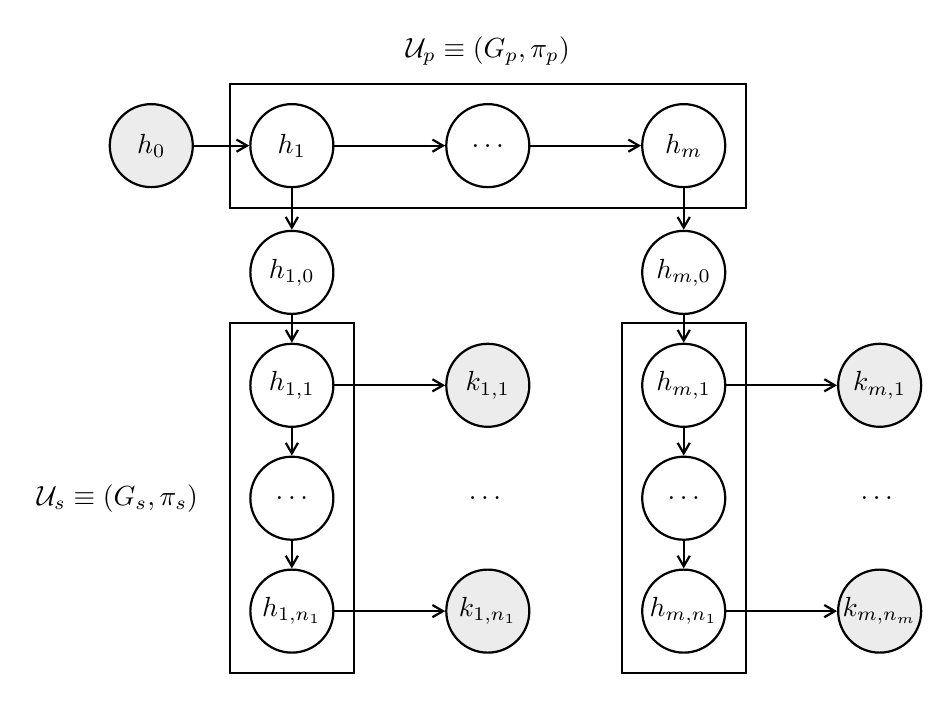
\begin{tikzpicture}
  \node[io] (x0) {$h_0$};
  \node[neuron,right=of x0] (x1)
  {$h_{1}$};
  \node[neuron,right=4em of x1] (dot)
  {$\ldots$}; 
  \node[neuron,right=4em of dot] (xM)
  {$h_{m}$};
  
  \node[neuron,below=1.5em of x1] (x1_0)
  {$h_{1,0}$};
  \node[neuron,below=1em of x1_0] (x1_1)
  {$h_{1,1}$};
  \node[neuron,below=1em of x1_1] (dot2)
  {$\ldots$};
  \node[right=4.5em of dot2] (dot3)
  {$\ldots$}; 
  \node[io,right=4em of x1_1] (o1_1)
  {$k_{1,1}$};
  \node[neuron,below=1em of dot2] (x1_N)
  {$h_{1, n_1}$};
  \node[io,right=4em of x1_N] (o1_N)
  {$k_{1, n_1}$};
  
  \node[neuron,below=1.5em of xM] (xM_0)
  {$h_{m,0}$};
  \node[neuron,below=1em of xM_0] (xM_1)
  {$h_{m,1}$};
  \node[neuron,below=1em of xM_1] (dot4)
  {$\ldots$};
  \node[right=4.5em of dot4] (dot5)
  {$\ldots$}; 
  \node[io,right=4em of xM_1] (oM_1)
  {$k_{m,1}$};
  \node[neuron,below=1em of dot4] (xM_N)
  {$h_{m, n_1}$};
  \node[io,right=4em of xM_N] (oM_N)
  {$k_{m, n_m}$};
  
  \node[left=1.5em of dot2] (gs)
  {$\mathcal{U}_s \equiv (G_s, \pi_s)$};
  \node[above=1em of dot] (gp)
  {$\mathcal{U}_p \equiv (G_p, \pi_p)$};
  \node[group,fit={(x1) (dot) (xM)}] (gr1) {};
  \node[group,fit={(x1_1) (dot2) (x1_N)}] (gr2) {};
  \node[group,fit={(xM_1) (dot4) (xM_N)}] (gr3) {};
  \draw[conn] (x0) -- (x1);
  \draw[conn] (x1) -- (dot);
  \draw[conn] (dot) -- (xM);
  
  \draw[conn] (x1) -- (x1_0);
  \draw[conn] (x1_0) -- (x1_1);
  \draw[conn] (x1_1) -- (dot2);
  \draw[conn] (dot2) -- (x1_N);
  \draw[conn] (x1_1) -- (o1_1);
  \draw[conn] (x1_N) -- (o1_N);
  
  \draw[conn] (xM) -- (xM_0);
  \draw[conn] (xM_0) -- (xM_1);
  \draw[conn] (xM_1) -- (dot4);
  \draw[conn] (dot4) -- (xM_N);
  \draw[conn] (xM_1) -- (oM_1);
  \draw[conn] (xM_N) -- (oM_N);
\end{tikzpicture}
\caption{Schematic of the kernel generator with nested units $\mathcal{U}_p$ and $\mathcal{U}_s$. Each component recursively computes its next hidden state and emission output using respective recurrent neural network $G_s$ and $G_p$. The termination probability at each generative step is determined by policies $\pi_p$ and $\pi_s$. The final candidate kernel expression is composed using Eq.~\eqref{c3-eq:general}.}
\label{c3-fig:generator}
\end{figure}
Our termination policy $\pi$ is then given by a pair of functions that correspond to these component networks and are modelled by simple feed-forward neural networks. Specifically, each function takes as input an intermediate kernel expression and estimates the probability that its respective component network should be terminated to yield the optimal kernel function. 

\begin{figure}
\centering
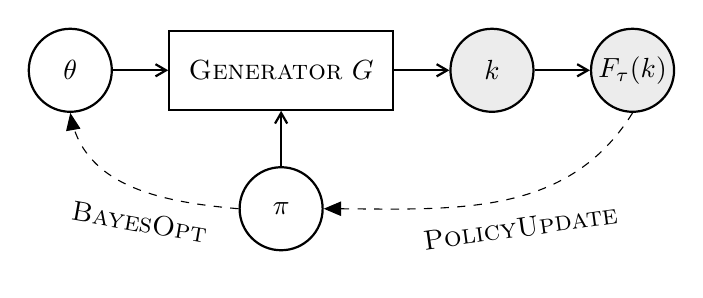
\begin{tikzpicture}
  \node[group2, minimum size=1cm] (g) {\textsc{Generator} $G$};
  \node[neuron, left=2em of g] (t) {$\theta$};
  \node[neuron, below=2em of g] (p) {$\pi$};
  \node[io, right=2em of g] (k) {$k$};
  \node[io, right=2em of k] (f) {$F_{\tau}(k)$};
  \draw[conn] (t) -- (g);
  \draw[conn] (p) -- (g);
  \draw[conn] (g) -- (k);
  \draw[conn] (k) -- (f);
  \draw [dashed,->] (f.south) to [out=-122,in=0] (p.east) node[below right=1.2em, rotate=8]{\ \ \ \ \ \ \ \textsc{PolicyUpdate}};
  \draw [dashed,->] (p.west) node[below left=0.5em, rotate=-10]{\textsc{BayesOpt}\ \ } to [out=-185,in=-80] (t.south);
\end{tikzpicture}
\caption{The generic workflow of \textsc{DTerGenS}. Given policy $\pi$, we employ BO to obtain generative weight candidate $\theta$ (Section~\ref{app-ks-subsec:theta}). Using the observed generative trajectory, we alternately update the policy distribution (Section~\ref{app-ks-subsec:pi}).}
\label{c3-fig:workflow}
\end{figure}

We propose a bi-level optimization scheme to sequentially optimize both these components. At every update iteration, we use the Bayesian optimization (BO) framework to obtain and evaluate a candidate generative weights $\theta$. Fixing a policy $\pi$ allows us to distill an concrete kernel expression from the induced generative trajectory and consequently obtain its respective performance. The partial trajectory obtained is then used to update the policy networks. A high-level overview of this algorithm is given in Fig.~\ref{c3-fig:workflow}. 

Although the use of BO is similar to~\citet{Lu18} and~\citet{Malkomes16}, specific considerations need to be applied to account for the differences in settings between our proposal and these approaches. For instance, a major technical challenge that arises in our formulation is that the semantics of our latent representations will dynamically change between BO iterations as the policy $\pi$ is updated. Explicitly, even though each $\theta$ encodes a unique generative trajectory, the performance obtained by querying $R_\tau$ also depends on the early stop decisions drawn from the current policy $\pi$. As such, it is necessary that our surrogate model can accurately capture the correlation between different instantiations of $\pi$.

To achieve this, we first impose Gaussian priors on the weights of our policy networks and further assume that termination policy $\pi$ is constructed at every iteration via sampling from the respective weight distributions. As each policy is now implicitly represented by a pair of distributions, we subsequently propose to estimate the correlation between two instantiations of $\pi$ via computing their corresponding Jensen-Shannon divergences, which are then incorporated into the BO surrogate model. Finally, given an observed (partial) trajectory at the end of each BO iteration, we further devise an update strategy for the weight distributions of $\pi$ via minimizing their expected deviation from the actual optimal stopping point. The full detail of our technical contributions and empirical demonstrations is given in Appendix~\ref{app:ks}.

\section{Results}
To demonstrate the performance of \textsc{DTerGenS}, we compare our method with the following benchmarks: (a) random search over the space of kernels with max length $L \leq 10$ (baseline); (b) \textsc{SVO}: Structure Variationally-Encoded Optimization~\cite{Lu18}, for which we train the VAE component using 25000 randomly generated kernel expressions with max length $L \leq 10$ (to show the advantage of generative search); and (c) our own algorithm with no stopping policy and fixing expression length $L = 2, 4, 8$. For (c), the termination of the secondary component is chosen at random, the termination of primary component is guaranteed upon reaching length $L$, and REMBO~\cite{Wang16} is used to optimize generative weights $\theta$. These benchmarks serve as ablation studies to demonstrate the advantage of having adaptive termination policies for the generative components. 

We first demonstrate that our kernel selection framework can accurately recover a synthetic kernel structure given observations simulated by its corresponding distribution. In particular, we arbitrarily construct several kernels with different complexities and show that in all scenarios, our method \textsc{DTerGens} outperformed other benchmarks in terms of recovery error (i.e., the Frobenius-norm of the distance between ground truth annd reconstructed covariance matrices). 

We further demonstrate the effectiveness of our approach on several real-world regression datasets, including: (1)~the DIABETES dataset~\cite{UCI_diabetes_data}, which contains 442 diabetes patient records; (2)~the MAUNA LOA dataset~\cite{mauna_loa_data}, which measures monthly average $\textrm{CO}_2$ concentration at the Mauna-Loa Observatory over 42 years; and (3)~the PROTEIN dataset~\cite{UCI_protein_data}, which features 45730 protein tertiary structures. Our empirical results show that \textsc{DTerGens} outperformed other benchmarks in terms of prediction errors, the implying the discovery of better kernel structures. 

The full detail of our experiments are given in Appendix~\ref{app:ks}. This work has been published at the International Conference on Machine Learning (2020).
\label{sec:kernel}

\chapter{Minimizer Sketch Design}
\label{c4:minimizer}
\section{Problem setting}
The minimizer scheme~\citep{roberts05,schleimer03} is a sampling method that selects length-$k$ substrings (i.e., $k$-mers) from a string such that sufficient information about the identity of the sequence is preserved, typically for comparison purpose. It is widely used to reduce memory consumption and run-time in bioinformatics applications such as genome assemblers~\citep{ye12}, read mappers~\citep{jain20,li18minimap2} and $k$-mer counters~\citep{deorowicz15kmc,erbert17gerbil}. 

Our discussion of the minimizer scheme will be grounded in sequences drawn from an arbitrary alphabet $\Sigma$. To begin, let us define some useful notations. Given some parameter $k$, a $(w,k)$-window is defined as a substring of length $w_k=w-k+1$, which contains exactly $w$ overlapping $k$-mers. Let $S \in \Sigma^{L+k-1}$ be sa string containing exactly $L$ overlapping $k$-mers and $L_w\triangleq L-w+1$ overlapping $(w,k)$-windows. Generally, we assume that $w\ll L$ and $k\ll L$, as is typical in most practical settings. We use the notations $\kappa^k_i$ and $\kappa^{w_k}_i$ to respectively denote the $i^{\text{th}}$ $k$-mer and the $i^{\text{th}}$ $(w, k)$-window in $S$. 

Generally, a $k$-mer sampling scheme is a function $\mathcal{X}$ such that $\mathcal{X}(S) \in 2^{[L]}$ returns a set of $k$-mer locations in $S$. The resulting sketch is given by the notation $\mathcal{K}(S; \mathcal{X}) \triangleq \{(\kappa^k_i, i)\}_{i \in \mathcal{X}(S)}$. Note that the sketch report tuples of both $k$-mer and index to distinguish identical $k$-mers sampled from different parts of $S$. We evaluate the performance of such a sampling scheme by computing its density~\citep{marcais17}, which is the fraction of sampled $k$-mers relative to the length of the target sequence:
\begin{eqnarray}
{D}(S; \mathcal{X}) &\triangleq& \frac{\left|\mathcal{K}(S; \mathcal{X}, r)\right|}{L} \ .
\label{c5-eq:density}
\end{eqnarray} 

\noindent The minimizer scheme \cite{schleimer03} is a $k$-mer sampling scheme that makes its sampling decisions based on an arbitrarily constructed total ordering on the $k$-mer set, which is represented by a permutation $\pi$. In particular, we define the minimizer scheme as follows:
\begin{definition}[Minimizer]
\label{c5-def:minimizer}
A minimizer scheme is characterized by a tuple of parameters $(w, k, \pi)$, where $w, k$ are defined above and $\pi$ is a total ordering on the set of all $k$-mers. We define the following selector function, which returns the lowest-ranked $k$-mer in some $(w,k)$-window of $S$: 
\begin{eqnarray}
m(\kappa^{w_k}_v; \pi) &\triangleq&  \underset{i \in [1, w]}{\mathrm{argmin}} \ \sum_{j \in [1,w]} \mathbb{I}(\kappa^k_{v+j-1} <_{\pi} \kappa^k_{v+i-1}) \ ,
\label{c5-eq:minimizer}
\end{eqnarray}
where $\kappa^k_{v+i-1}$ denotes the $i^{\text{th}}$ $k$-mer in the window $\kappa^{w_k}_v$ and $\mathbb{I}(\kappa <_{\pi} \kappa')$ denotes the event that $\kappa$ precedes $\kappa'$ in $\pi$ for some $\kappa,\kappa' \in \Sigma^k$. The minimizer sampling function is then given by:
\begin{eqnarray}
\mathcal{M}(S;w,k,\pi) \triangleq \{i + m(\kappa^{w_k}_i;\pi)\}_{i\in[L_w]} \ ,
\label{eq:mnzsketch}
\end{eqnarray}
which iteratively applies $m$ on every window in $S$.
\end{definition}
 A low-density minimizer scheme achieves three desiderata: (1)~the sketch is compact and will offer significant cost saving to downstream applications; (2)~every $(w,k)$-window in $S$ overlaps at least one $k$-mer in the sketch; and (3)~identical windows are represented by the same $k$-mer due to the deterministic sampling protocol. These properties give rise the minimizer sketch design (MSD) problem below.
\begin{definition}[Low Density Minimizer Sketch Design]
\label{c5-def:minimizerproblem}
Let $S$ be a string defined as above. Suppose $w$, $k$ and $r$ are given as application-specific parameters, the minimizer selection problem is defined as:
\begin{eqnarray} 
 \pi_\ast &=& \underset{\pi \in \Pi(\Sigma^k)} {\mathrm{argmin}} \ \mathcal{D}(S; \mathcal{M}(\pi)) \ ,
\label{c5-eq:obj}
\end{eqnarray}
where $\Pi(\Sigma^k)$ denotes the set of all $k$-mer permutations in $\Sigma^k$ and we write $\mathcal{M}(\pi)$ to clearly show the dependency of $\mathcal{M}$ on the $k$-mer ordering $\pi$, which is being optimized.
\end{definition} 

\noindent Another recently suggested sketching desiderata~\citep{edgar2021syncmers} is that two substrings differing only by a few mutations are likely represented by the same $k$-mer in the sketch. \citet{edgar2021syncmers}~argues that the density metric above is not sufficient to capture this, and hence proposes an alternative metric called \textit{conservation}:
\begin{eqnarray}
{C}(S; \mathcal{X}) &\triangleq& \mathbb{E}_{S'}\left[\frac{\left|\mathcal{K}(S; \mathcal{X}) \cap \mathcal{K}(S'; \mathcal{X})\right|}{L}\right]\ ,
\label{c5-eq:cons}
\end{eqnarray} 
which measures the expected fraction of selected $k$-mers (relative to the length of $S$) that are preserved under random mutation (i.e., higher is better). Here, $S'$ is a copy of $S$ with randomly substituted characters and the conservation metric is expected over the distribution of $S'$. To obtain high conservation sketches \citet{edgar2021syncmers} also proposes another sketching method called \emph{syncmers}.
\begin{definition}[Syncmer]
\label{c5-def:syncmer}
A syncmer scheme is defined by a tuple of parameters $(k, s, t, \pi)$, where $k$ similarly denotes the substring length to be sampled (i.e., $k$-mers) and $s, t \in [1,k]$. Here, $\pi$ is a permutation of all $s$-mers in $\Sigma^s$. Similar to Definition~\ref{c5-def:minimizer}, we also define a selector function, which now returns the lowest-ranked $s$-mer in some $k$-mer of $S$: 
\begin{eqnarray}
m(\kappa^k_v; \pi) &\triangleq& \underset{i \in [1,k]}{\argmin} \sum_{j\in[1,k_s]} \mathbb{I}(\kappa^s_{v+j-1} <_{\pi} \kappa^s_{v+i-1}) \ ,
\end{eqnarray}
where $k_s \triangleq k-s+1$ denotes the number of overlapping $s$-mer in a $k$-mer. The syncmer sampling function is then specified by iteratively sampling any $k$-mer such that its lowest-ranked $s$-mer is at the $t^{\text{th}}$ position:
\begin{eqnarray}
\mathcal{O}_t(S; k, s, \pi) \triangleq \{i \mid m(\kappa^k_i; \pi) = t\}_{i\in [L]} \ .
\end{eqnarray}
We specially choose to write $t$ as a subscript since syncmer schemes with similar $k, s, \pi$ initialization and different offset $t$ are theoretically related, as shown below in the technical approach.
\end{definition}
Although there has been no explicit sketch design method developed for syncmers (i.e., optimizing the $s$-mer permutation $\pi$), \citet{edgar2021syncmers}~and \citet{shaw2021theory}~have empirically observed that the syncmer method is capable of simultaneously achieving both lower density and higher conservation than the minimizer method when both use a random ordering. Nonetheless, no formal relationship has been established between the two methods due to the lack of a convention to compare them.

This chapter explores a new approach for solving the minimizer sketch design problem via a differentiable reformulation of the permutation learning task in Definition~\ref{c5-def:minimizer}, called \textsc{DeepMinimizer}. We then derive the first theoretical relationship between the density and conservation metrics; as well as between the minimizer and syncmer methods. This new insight allows us to (1)~unify minimizers and syncmers under a generalized notion of sequence sketching called \textit{masked minimizer}; and (2)~extend our \textsc{DeepMinimizer} framework to automate \textit{masked minimizer} sketch design.

\section{Related work}
\subsection{UHS-based methods} Most existing minimizer selection schemes with performance guarantees over random sequences are based on the theory of universal hitting sets (UHS)~\citep{marcais18,orenstein17}. Particularly, a $(w,k)$-UHS is defined as a set of $k$-mers such that every window of length $w$ (from any possible sequence) contains at least one of its elements. Every UHS subsequently defines a family of corresponding minimizer schemes whose expected densities on random sequences can be upper-bounded in terms of the UHS size~\citep{marcais17}. As such, to obtain minimizers with provably low density, it suffices to construct small UHS, which is the common objective of many existing approaches~\citep{marcais17,ekim20pasha,zheng20miniception}. These methods, however, rely on the unrealistic assumption that the target sequences follow a uniform distribution~\citep{zhang07}. As such, there tends to be little correspondence between the provable upper-bound on expected density and the actual density measured on a target sequence. 

\subsection{Heuristic methods} Several minimizer construction schemes rank $k$-mers based on their frequencies in the target sequence~\citep{chikhi16,jain20b}, such that infrequent $k$-mers are more likely to be chosen as minimizers. These constructions nonetheless rely on the assumption that infrequent $k$-mers are spread apart and ideally correspond to a sparse sampling. Another greedy approach is to sequentially remove k-mers from an arbitrarily constructed UHS, as long as the resulting set still hits every $w$-long window on the target sequence~\citep{deblasio19}. Though this helps to fine-tune a given UHS with respect to the sequence of interest, there is no guarantee that such an initial set will yield the optimal solution after pruning.

\subsection{Polar set construction} Recently, a novel class of minimizer constructions was proposed based on polar sets of $k$-mers, whose elements are sufficiently far apart on the target sequence~\citep{zheng21}. The sketch size induced by such a polar set is shown to be tightly bounded with respect to its cardinality. This reveals an alternate route to low-density minimizer schemes through searching for the minimal polar set. Unfortunately, this proxy objective is NP-hard and currently approximated by a greedy construction~\citep{zheng21}, which can be sub-optimal in practice.

\section{Differentiable reformulation of the MSD problem}
\subsection{Motivation}
The technical challenges of the MSD problem described above arise due to two factors. First, the search space is factorially large in terms of $k$. Exhaustively searching this domain of $k$-mer permutations would suffice for very small $k$, but will quickly become intractable for larger values of $k$ that are typically used in many practical applications. Second, the density minimizing objective is discrete, hence difficult to be optimized via standard techniques. 

All existing MSD frameworks approach this optimization problem by approximating its permutation search space (i.e., space of total $k$-mer orderings) with the space of partial $k$-mer orderings that satisfy certain surrogate properties. For example,~\citet{marcais17,marcais18,ekim20pasha,zheng20miniception} adopt the universal hitting set (UHS) approximation which imposes that all $k$-mers in a selected UHS will be ranked with lower priorities than those outside. The polar set (PS) approximation proposed by~\citet{zheng21} is similar in spirit, but uses a different set of surrogate properties to construct these partial orderings.

The main advantage of these strategies is that they reduce the permutation learning objective in Definition~\ref{c5-def:minimizerproblem} to finding the most compact construction of such surrogate sets, which is relatively simpler to achieve. However, these approximations either rely on unrealistic assumptions about the target sequence, such as its characters are uniformly distributed (e.g., UHS-based methods~\cite{marcais17,marcais18,ekim20pasha,zheng20miniception}); or remain a challenging discrete objective that can only be solved via greedy heuristics (e.g., the PS method~\cite{zheng21}). Furthermore, both of these approximation schemes can be viewed as domain restriction techniques where the sets of active candidates are confined to UHS/PS-induced permutations. Nonetheless, there is no guarantee that these active sets would necessarily contain the optimal solution.

To overcome these challenges, we instead propose a re-parameterization of the original permutation learning problem, which implicitly casts the $k$-mer permutation $\pi$ as a function $f_\pi: \Sigma^k \rightarrow [0,1]$ that assign continuous scores to $k$-mers in $\Sigma^k$. Every \emph{valid} candidate function must be a consistent scoring scheme (i.e., a $k$-mer will get the same score regardless of its position and local neighborhood in the target sequence), such that a permutation can always be recovered via sorting the scores. Modelling the space of such valid functions with a deep neural network, we subsequently propose to cast the MSD problem as a deep learning optimization task with respect to the density objective in Definition~\ref{c5-def:minimizerproblem}. We further note that, unlike existing approximations, the candidate set encoded by our re-parameterization can theoretically approach the unrestricted permutation domain $\Pi(\Sigma^k)$ given a sufficiently expressive network architecture.

\begin{figure}[ht]
\centering
\begin{tabular}{c}
\includegraphics[width=0.95\columnwidth]{minimizer_plots/Schematic.png} 
\end{tabular}
\caption{The \textsc{DeepMinimizer} framework is comprised of two continuous $k$-mer scoring schemes that correspond to different aspects of a low-density minimizer: \textsc{PriorityNet} assigns scores to $k$-mers in the target sequence such that a total ordering can be recovered via simple sorting; whereas \textsc{TemplateNet} relaxes this consistency constraint to achieve a low-density sketch. Minimizing the distance between their outputs is expected to yield a consensus solution that simultaneously exhibits both properties.}
\label{c5-fig:prioritynet}
\end{figure}
Nonetheless, standard backpropagation methods~\citep{kingma14adam} cannot be directly applied to optimize the density metric, which is discrete and does not have an analytic gradient with respect to the network parameters. To address this challenge, we further adopt a similar approach to the proposed KS framework in Chapter~\ref{c3:kernel}, which hierarchically approximates the search task with multiple sub-tasks that can each be solved more efficiently. In the MSD context, these sub-tasks manifest as a pair of complementary neural networks called \textsc{PriorityNet} and \textsc{TemplateNet}. In particular, the \textsc{PriorityNet} component is parameterized such that it always outputs consistent scoring and is tasked to encode the candidate function space of the minimizer scheme. On the other hand, the \textsc{TemplateNet} component relaxes this consistency constraint in exchange for the ability to encode desirable score assignments (but potentially unmeaningful since it might not be possible to recover a proper minimizer scheme). While the KS framework in Chapter~\ref{c3:kernel} adopts a bi-level optimization approach to alternately solve its sub-tasks (i.e., generative trajectory selection and early stopping policy), both components in this MSD scenario can be simultaneously learned via minimizing the divergence between their outputs, hence resulting in the first differentiable relaxation for the MSD problem. A high-level schematic of our approach is shown in Fig.~\ref{c5-fig:prioritynet}. Last, we propose to demonstrate that our method, titled \textsc{DeepMinimizer} is highly-efficient and capable of finding minimizer schemes that yield significantly more compact sketches on multiple human genome benchmarks. The remainder of this chapter will now provide a summary of our technical approach, which will be presented in details in Appendix~\ref{app:maskmnz} along with our empirical findings.

\subsection{Technical Approach}
Using the notion of the scoring function $f_\pi$, the selector function in Definition~\ref{c5-def:minimizer} can be written as:
\begin{eqnarray}
m(\kappa^{w_k}_v; \alpha) &\triangleq& \underset{i \in [1,w]}{\argmin} \ f_\pi\left(\kappa^k_{v+i-1}; \alpha\right) \ ,
\label{eq:mnzselector}
\end{eqnarray}
where $f: \Sigma^{k} \rightarrow [0, 1]$ is parameterized by a convolutional neural network with weight $\alpha$. The architecture of this network (as discussed in Appendix~\ref{app:maskmnz}) guarantees that $f$ is a valid scoring function (i.e., we can always recover a total ordering over all $k$-mers), that is, for all pairs of indices $i, j \in [L]$, we have:
\begin{eqnarray}
\kappa^k_i = \kappa^k_j &\implies& f(\kappa^k_i) = f(\kappa^k_j) \ .
\end{eqnarray}

\noindent For clarity, we will write the density metric as $\mathcal{D}(S; \mathcal{M}(\alpha))$ to clearly establish the change in parameterization. As discussed in the previous section, $f$ cannot be efficiently optimized with gradient back-propagation methods since the derivative $\frac{\partial\mathcal{D}(S; \mathcal{M}(\alpha))}{\partial\alpha}$ does not exist. To work around this, we introduce a proxy optimization objective that approximates $\mathcal{D}(S; \mathcal{M}(\alpha))$ via coupling $f$ with a positional scoring function $g: [L] \rightarrow [0,1]$ parameterized by weight $\beta$. Unlike $f$, which assigns $k$-mers scores based on their contents, $g$ assigns $k$-mers scores based on their positions in $S$ and is likely not a valid scoring function, i.e., $\kappa^k_i = \kappa^k_j \centernot\implies g(i) = g(j)$. Nonetheless, the context-free function $g$ can be used to generate a $k$-mer sketch by adapting Eq.~\ref{eq:mnzsketch} as:
\begin{eqnarray}
\mathcal{T}(S; \beta) \triangleq \left\{i + \underset{j\in[1,w]}{\argmin} \ g(i+j-1; \beta)\right\}_{i \in [L_w]} \ .
\end{eqnarray}
The \emph{template} $k$-mer sampling scheme $\mathcal{T}$ does not have the same desiderata as a minimizer sketch, but we can guarantee that the sketch density is equal to that of an optimal minimizer sketch through carefully constructing $g$, i.e., $\mathcal{D}(S; \mathcal{T}(\beta)) \simeq 1/w$. As $\mathcal{K}(S; \mathcal{M}(\alpha), r)$ corresponds exactly to a minimizer sketch and $\mathcal{K}(S; \mathcal{T}(\beta), r)$ approximates the low-density objective, this reveals an interesting factorization of the search task, and therefore an alternative pathway to the optimal solution through finding a \emph{consensus solution} between the two sketches. Formally, let $\mathbf{f}(S,\alpha) = [f(\kappa^k_i;\alpha)]_{i\in[L]}$ and $\mathbf{g}(\beta) = [g(i)]_{i\in[L]}$ respectively denote the concatenated score vectors that $f$ and $g$ assign to $k$-mers in $S$, we then characterize this consensus solution as a joint instantiation of $\alpha$ and $\beta$ such that some distance metric $\Delta$ between $\mathbf{f}(S,\alpha)$ and $\mathbf{g}(\beta)$ is minimized. Explicitly, this results in the following optimization objective:
\begin{eqnarray}
(\alpha_\ast,\beta_\ast) &\triangleq& \underset{\alpha, \beta}{\argmin} \ \Delta\left(\mathbf{f}(S,\alpha),\mathbf{g}(\beta)\right) \ ,
\end{eqnarray}
which is fully differentiable with respect to weights $\alpha$ and $\beta$. We fully describe our approach, including the parameterizations of $f$, $g$ and the distance metric $\Delta$ in Appendix~\ref{app:maskmnz}.
\section{Unifying minimizer and syncmer sketching methods}
\subsection{Motivation}
Although both minimizers and syncmers employ the same concept of sampling based on a substring total ordering, a minimizer scheme that uses an $s$-mer ordering will directly report $s$-mers in its sketch, whereas a syncmer scheme parameterized by the same ordering will typically report longer $k$-mers. Due to this mismatch in representation, existing work~\cite{edgar2021syncmers,shaw2021theory} all chose to compare schemes that report similar-sized substrings regardless of their ordering choices, which results in an asymmetry of information among their sketches and prevents the derivation of any meaningful correspondence between minimizers and syncmers. 

This shortcoming motivates a revision of the comparability notion for sketching methods. In particular, we advocate comparing schemes that use the same substring ordering to make sampling decisions. This new mode of comparison allows us to explicitly bound the density and conservation gaps between minimizers and syncmers. Building on this theoretical result, we further propose a novel concept of masked minimizers that unify both minimizers and syncmers. The masked minimizer scheme combines the standard minimizer sampling with an additional sub-sampling step, which applies a binary mask filter to the $k$-mer selection at every window. Interestingly, varying this mask parameter induces a spectrum of comparable schemes and reveals a methodical approach to derive comparable sketching schemes. Last, we propose an extension of the \textsc{DeepMinimizer} method to optimize the masked minimizer scheme with respect to a novel sketching metric called the \emph{generalized sketch score} (GSS), which combines both  density and conservation metrics, resulting in the first formal protocol to compare sequence sketching methods.
\subsection{Technical approach}
To explicitly reason about the difference in terms of sketch representation between minimizers and syncmers, we introduce the notion of a reporting function $r$, which maps the sampled locations in $\mathcal{X}(S)$ to tuples of substrings and locations. That is, the reported sketch is now constructed as $\mathcal{K}(S; \mathcal{X}, r) \triangleq \{r(i)\}_{i \in \mathcal{X}(S)}$. Setting $r(i) = (\kappa^k_i, i)$ recovers both Definition~\ref{c5-def:minimizer} of a minimizer scheme with parameters $w, k$ and $\pi_m \in \Pi(\Sigma^k)$; and Definition~\ref{c5-def:syncmer} of a syncmer scheme with parameters $k, s, t$ and $\pi_o \in \Pi(\Sigma^s)$. Since these methods both report $k$-mers, they are traditionally deemed comparable.

This mode of comparison, however, does not facilitate a theoretical analysis of their performance differences (i.e., in terms of density and conservation metrics), as different information bases are used to enact the sampling decisions of a length-$k$ minimizer and syncmer. In particular, $(w, k)$-minimizer schemes use total $k$-mer orderings to perform sampling, whereas $(k, s, t)$-syncmer schemes use total $s$-mer orderings, with $s \leq k$. We note that these bases are only comparable when setting $s=k$, but doing so results in trivial syncmer schemes that selects every $k$-mer in $S$. 

To correct this asymmetry of information, we propose the notion of $\pi$-comparable minimizers and syncmers, which are schemes that employ the same ordering $\pi$. For example, the $(w, k, \pi)$-minimizer and the $(w_k, k, t, \pi)$-syncmer schemes with $w_k\triangleq w+k-1$ and any $t \leq w$, which respectively report $k$-mers and $w_k$-mers, are $\pi$-comparable. To normalize the difference in representation, we replace the default $w_k$-mer reporting function $r(i)=(\kappa^{w_k}_i, i)$ of the above syncmer scheme with the $k$-syncmer reporting function $r'(i)=(\kappa^k_{i+t}, i+t)$. As both reporting functions are one-to-one mappings of the selected locations, this substitution results in a semantically equivalent \textit{shifted} syncmer scheme.

This translation of the reporting function aligns our proposed comparison with the traditional perspective of comparability and presents an invariant substring ranking behavior among the compared schemes, which subsequently allows us to derive explicit bounds on their density and conservation gaps. In particular, we prove that the density and conservation of any syncmer on a specific sequence $S$ are respectively upper-bounded and almost surely upper-bounded by that of its $\pi$-comparable minimizer, thus establishing the first theoretical correspondence between $\pi$-comparable schemes. Our theoretical result is summarized in Theorem~\ref{c5-theo:1}, whose detailed proof is given Appendix~\ref{app:maskmnz}.
\begin{theorem}[$\pi$-comparability defines a correspondence between minimizers and syncmers] For \linebreak every syncmer scheme  $(\mathcal{O}_t, r')$, there exists a comparable minimizer scheme $\mathcal{M}$ whose reporting function $r$ is translated from $r'$ with an offset $t$, such that the following bounds hold for every $S \in \Sigma^{L+k-1}$: 
\begin{eqnarray}
D(S; \mathcal{O}_t,r') \ \leq 
 \ D(S; \mathcal{M},r) \qquad \text{and} \qquad  C(S; \mathcal{O}_t,r') \ \leq \ C(S; \mathcal{M},r) + \frac{t}{L} \ .
\end{eqnarray}
\label{c5-theo:1}
\end{theorem}
We then further show that any syncmer scheme can be recovered given a $\pi$-comparable minimizer $\mathcal{M}$ via sub-sampling the set of locations selected by $\mathcal{M}$. We write this sub-sampling rule as follows:
\begin{eqnarray}
\mathcal{O}_t(S) &=& \left\{
i - t \mid \left\|    \overrightarrow{m}(\kappa^{w_k}_{i-t};\pi) \otimes \mathbf{e}_t
\right\|_1 > 0
\right\}_{i \in \mathcal{M}(S)} \ ,
\end{eqnarray}
where $\overrightarrow{m}(\kappa^{w_k};\pi) \triangleq [\mathbb{I}(j=m(\kappa^{w_k}; \pi))]_{j\in[w]}$ is the one-hot representation of the $k$-mer selection result at some arbitrary window $\kappa^{w_k}$ using the selector function $m$; $\mathbf{e}_t$ denotes the one-hot vector with a non-zero entry on the $t^{\text{th}}$ row; and $\otimes$ denotes the pointwise multiplication operator. The sub-sampling condition above checks if any position remains selected after filtering with $\mathbf{e}_t$ (in which case, it must be the $t^{\text{th}}$ position). Interestingly, this sub-sampling rule can be generalized by replacing $\mathbf{e}_t$ with any arbitrary $w$-dimensional binary mask $\nu \in \{0,1\}^w$. For example, setting $\nu=\mathbf{1}_w$ trivially recovers the standard minimizer scheme (without applying the offset $t$). Given a set of minimizer-sampled locations $\mathcal{M}(S)$,  varying $\nu$ yields a total of $2^w$ $\pi$-comparable schemes, leading to a unifying method called \textit{masked minimizers}. 
\begin{definition}[Masked minimizers] 
The sampling function of a masked minimizer scheme is characterized by a tuple of parameters $(w, k, \pi, \nu)$, where $w,k,\pi$ correspond to standard minimizer parameters, and $\nu\in\{0,1\}^w$ is a $w$-dimensional binary vector. The masked minimizer sampling function is given by:
\begin{eqnarray}
\mathcal{V}(S; w,k,\pi,\nu) \ \triangleq \ \{i + m(\kappa^{w_k}_i; \pi) \mid \zeta(\kappa^{w_k}_i, \nu)\}_{i\in[L_w]} \ ,
\end{eqnarray}
where $\zeta(\kappa^{w_k}_i, \nu) \triangleq \|\overrightarrow{m}_\pi(\kappa^{w_k}_i) \otimes \nu]\|_1 > 0$ denotes the event that the selection at the $i^{\text{th}}$ window remains sampled after applying the sub-sampling mask.
\end{definition}

\noindent We also show that improving density places an upper-bound on how much conservation can be improved and vice versa, which implies that neither objective should be considered independently of one another. To account for this trade-off, we propose a new metric called the \emph{generalized sketch score} (GSS):
\begin{eqnarray}
G(S; \mathcal{X}, r, w) &\triangleq& \frac{C(S;\mathcal{X},r)}{D(S;\mathcal{X},r)} \cdot \frac{1}{L_w} \sum_{i=1}^{L_w} V_i(S; \mathcal{X}, w) \ ,
\end{eqnarray}
where $V_i(S;\mathcal{X}, w) \triangleq 1 - \prod_{j=i}^{i+w-1} \mathbb{I}(j \not\in \mathcal{X}(S))$ is the indicator variable of the event that the window $\kappa^{w_k}_i$ overlaps at least one sampled location in $\mathcal{X}(S)$. The GSS metric seeks to capture the trade-off between density and conservation via the ratio $C(S;\mathcal{X}, r)/D(S;\mathcal{X},r)$ and further prevents possible trivial exploitation with the \emph{coverage} term $\sum_{i=1}^{L_w} V_i(S; \mathcal{X}, w)$. We provide the full explanation regarding the benefits of this metric in Appendix~\ref{app:maskmnz}.

Finally, we propose an extension of the \textsc{DeepMinimizer} method to optimize a masked minimizer scheme with respect to the GSS metric. In particular, our new objective is given as a bilvel optimization:
\begin{eqnarray}
(\alpha_\ast,\beta_\ast) &\triangleq& \underset{\alpha, \beta}{\argmin} \ \Delta\left(\mathbf{f}(S,\alpha),\mathbf{g}(\beta)\right) + \sum_{i=1}^n \Delta\left(\mathbf{f}(S_i,\alpha),\mathbf{f}(S, \alpha)\right) \ , \nonumber \\
\quad \nu_\ast &\triangleq& \underset{\nu}{\argmin} \ G(S; \mathcal{V}(\alpha_\ast), r, w) \ ,
\end{eqnarray}
where $S_1, S_2, \dots, S_n$ denote $n$ randomly sampled mutations of $S$; $\Delta$, $\mathbf{f}$ and $\mathbf{g}$ are previously defined in the technical exposition of the \textsc{DeepMinimizer} method. The first optimization adds an extra term to the \textsc{DeepMinimizer} loss, which measures the expected distance between each priority vector $\mathbf{f}(S_i,\alpha)$ for mutated sequence $S_i$ and the original template vector $\mathbf{f}(S,\alpha)$. As the priority vector is a surrogate for the actual discrete $k$-mer selection, minimizing this term will likely improve the stability of selection (i.e., conservation) when the sequence is subjected to random mutations. The second optimization, on the other hand, is written as a greedy search to find the optimal mask given an ordering induced by the parameter $\alpha_\ast$ obtained from the first optimization. We detail our approach in Appendix~\ref{app:maskmnz}.

\section{Results}
To demonstrate the performance of \textsc{DeepMinimizer}, we compare our method with the following benchmarks: (a)~A random minimizer (the total ordering $\pi$ is uniformly sampled); (b) \textsc{Miniception}~\cite{zheng20miniception}; (c) \textsc{PASHA}~\cite{ekim20pasha}; and (d) \textsc{PolarSet}~\cite{zheng21}. We use the following sequence benchmarks to conduct our empirical study: (a)~human chromosome 1 (\textsc{Chr1}); (b) ~human chromosome X (\textsc{ChrX}); (c) ~the centromere region of chromosome X (\textsc{ChrXC}); (d) ~the full human genome (\textsc{Hg38}). The full details of these sequences are given in Appendix~\ref{app:maskmnz}.

We first compare the minimizer sketch before and after training with \textsc{DeepMinimizer} to demonstrate that \textsc{DeepMinimizer} results in a sparse selection of $k$-mers in the target sequence. Across many settings of $w$ and $k$, we show that \textsc{DeepMinimizer} consistently converges to a low-density sketch, which shows that our objective function correlates well with the density metric. We also conduct ablation studies to study the effect of different template functions and distance functions, which justify our empirical choices. 

To demonstrate the effectiveness of our masked minimizers unification approach and justify our theoretical insight, we further conduct extra experiments to answer the following questions:
(1)~Are density and conservation adversarially related? (2)~How do $\pi$-comparable schemes perform relative to one another under the proposed metric GSS? (3)~Can mask optimization improve the overall performance of both minimizer and syncmer? Through these demonstrations, we confirm our theoretical understanding of various sketching metrics and the relationship among $\pi$-comparable schemes, as well as demonstrate the efficiency of our proposed optimization method.

Our experiments show that density and conservation metrics indeed have an adversarial relationship. In addition, our masked minimizer training method is highly effective in optimizing their trade-off. We demonstrate this effectiveness in many settings of $w, k$ and binary mask $\nu$. Last, we also demonstrate that selecting an optimal mask can have significant effect on the GSS of sketching methods. We test this on sequence patterns that are known to be difficult for standard minimizer methods and show that our approach are capable of finding masks that improve the performance.

We give the full details of our empirical study to Appendix~\ref{app:maskmnz}. Our work on the \textsc{DeepMinimizer} method has been published at the International Conference on Research in Computational Molecular Biology (RECOMB 2022). Our work on the unifying masked minimizer approach is currently under review for RECOMB 2023.
\label{sec:minimizer}

\chapter{Neural Architecture Search}
\label{c5:nas}
\section{Problem setting}
Neural network architecture is the core element of deep learning's success on many perceptual tasks such as computer vision~\cite{lecun2015lenet} and natural language processing~\cite{vaswani2017attention}. Even though most renowned architectures in deep learning literature are hand-designed by domain experts, recent studies~\cite{zoph2016,hu2020,xie2018} have suggested that searching for an optimal design that composes well-known building blocks can significantly improve performances in many task domains. Formally, a neural network architecture can be written as a hierarchical feature extractor which explicitly takes the form of a directed acyclic graph $G\triangleq(V, E)$, where $V$ and $E$ respectively denote the sets of nodes and edges in $G$. Each node $v\in V$ denotes an intermediate feature representation $z_v$, which has been arbitrarily transformed from some input $\mathbf{x} \in \mathbb{R}^d$. We often associate $\mathbf{x}$ and the output of the network with a source node $v_s$ and a sink node $v_t$, respectively. Each edge $e \equiv (v,v') \in E$ encodes an operator $o_e$ that transforms $z_v$ and forwards the result to $v'$ to be aggregated as $z_{v'}$. The computation of any intermediate representation in $G$ can then be recursively defined as:
\begin{eqnarray}
z_{v'} \triangleq \sum_{(v, v') \in E} o_{(v,v')}(z_v) \ ,
\end{eqnarray} 
where we have assumed a simple additive aggregation rule for simplicity. 

In a typical neural architecture search task, there are two design choices to be made: (1) the flow of information determined by the topology of $G$; and (2) the corresponding transformations of data features encoded by the edge operators $o_e$ for every $e \in E$. To ensure feasibility, the space of edge operators is often restricted to a small, finite set $\mathcal{O}$ of well-known layers, such as linear transformation, convolution and pooling, thus reducing the problem to finding an optimal mapping $m: E \rightarrow \mathcal{O}$ that assigns an operator in $\mathcal{O}$ for every edge. Similar to the setting of the kernel selection problem, we are also interested in only representing the \emph{categorical types} of these layers in $\mathcal{O}$, which do not include specific parameters whose optimization is well studied (i.e., layer weights) or must be chosen to ensure the mathematical consistency of the network (i.e., layer dimensions). In particular, given a selected layer type, the learning/setting of these parameters is implicitly incorporated into the performance measuring function.

On the other hand, designing the search space for $G$ is still an active research direction in which no conclusive insight has been reached regarding the best instantiation. This thesis thus focuses on a common practice proposed by~\citet{bender2018understanding}, which uses an over-parameterized graph $\mathcal{G}=(\mathcal{V},\mathcal{E})$ to implicitly define this space. That is, a candidate graph $G=(V, E)$ can be obtained by selecting subsets of nodes $V \subseteq \mathcal{V}$ and edges $E \subseteq \mathcal{E}$ such that $G$ is connected and contains both the source node $v_s$ and sink node $v_t$. We note that this pruning step can be trivially modelled by including a null layer in $\mathcal{O}$, which outputs zero regardless of the input feature, such that whenever this layer is selected, the edge it represents is considered inactive in the candidate graph. Finally, the neural architecture search problem on an overparameterized search space can be described as follows:

\begin{definition} [Neural Architecture Search]
Let $\tau \triangleq \{\mathcal{G},\mathcal{O},\mathcal{D}\}$ describe a neural architecture search task where $\mathcal{G}=(\mathcal{V},\mathcal{E})$ denotes an over-parameterized computation graph; $\mathcal{O}$ denotes the set of all edge operators; and $\mathcal{D}$ is the provided observations (i.e., train/validation/test data). We further let $\mathcal{M}$ be the set of all mappings $m: \mathcal{E} \rightarrow \mathcal{O}$ that assign a feature mapper for every edge in $\mathcal{G}$, thus inducing a unique architecture. Finally, let $F_\tau: \mathcal{M} \rightarrow \mathbb{R}$ be the performance measuring function of this task, which (1)~executes a well-defined algorithmic procedure to optimize the parameters of the selected operators (e.g., applying gradient descent update with respect to the cross-entropy loss until convergence) and (2)~returns the predictive accuracy evaluated on the test set. Then, the neural architecture search problem is succinctly stated as:
\begin{eqnarray}
m_\ast &=& \underset{m \in \mathcal{M}}{\mathrm{argmax}} \  F_\tau(m) \ ,
\end{eqnarray}
where $m_\ast$ denotes the optimally performing assignment function with respect to $\tau$.
\label{c4-def:nasproblem}
\end{definition}
We note that the problem statement above is specifically written for a single-task scenario, for which only one instance of $\tau$ requires optimal configuration. In this thesis, we further consider a new setting for neural architecture search, which focuses on concurrently configuring a set of $n$ related tasks $\boldsymbol{\tau} \triangleq \{\tau_1, \tau_2 \dots \tau_n\}$. We state the problem as follows:

\begin{definition} [Multi-task Neural Architecture Search]
Let $\boldsymbol{\tau} \triangleq \{\tau_1, \tau_2 \dots \tau_n\}$ be a set of neural architecture search tasks such that every task $\tau_i \triangleq \{\mathcal{G},\mathcal{O},\mathcal{D}_i\}$ shares the same search space $\mathcal{G}$ and the operator set $\mathcal{O}$, but differs from one another by the given task data $\mathcal{D}_i$.
Using the same notation of $\mathcal{M}$ in Definition~\ref{c4-def:nasproblem} and let $\mathbf{m} = \{m_1, m_2 \dots m_n\}$ be a collection of mappers in $\mathcal{M}$, where each $m_i$ corresponds to a candidate architecture for task $\tau_i$. The performance measuring function for the multi-task NAS problem is then given by averaging the per-task performance:
\begin{eqnarray}
F_{\boldsymbol{\tau}}(\mathbf{m}) &\triangleq& \frac{1}{n}\sum_{i=1}^n  F_{\tau_i}(m_i) \ .
\end{eqnarray}
Finally, we state the multi-task NAS objective as the following optimization task:
\begin{eqnarray}
\mathbf{m}_\ast &=& \underset{\mathbf{m} \subset \mathcal{M}}{\mathrm{argmax}} \  F_{\boldsymbol{\tau}}(\mathbf{m}) \ .
\end{eqnarray}
\label{c4-def:horizontalnas}
\end{definition}

\section{Related work}
The NAS literature can generally be classified into two separate lines of research: (1) search space design and (2) search strategy. As briefly mentioned above, this thesis will adopt the over-parameterized search space proposed by~\citet{bender2018understanding} and focus on developing new search strategies under this paradigm. This section provides a brief summary of various NAS methods in this direction (which we will simply refer to as NAS from this point onward) and some preliminary works in the multi-task NAS domain.
\subsection{Cell-based over-parameterized search space}
Most NAS methods converge on a cell-based organization of the over-parameterized network search space that was inspired by~\citet{pham2018}. This entails factoring the search space graph $\mathcal{G}$ into a linear chain of modular cell blocks, each serves as an over-parameterized network by itself. Every cell has its own source and sink node, which respectively receives the output of its previous cell and forwards its own output to the next cell. The NAS outcome is then the combined edge selection for all cells in $\mathcal{G}$, which is then achieved by specific search strategies.

\subsection{Scheduled dropout}
One major challenge of NAS is the expensive cost of evaluating candidate architectures, which involves sufficient training of the selected layer weights. \citet{bender2018understanding}~proposes to isolate this bottleneck from the performance measuring function through optimizing the entire over-parameterized network $\mathcal{G}$ once before conducting edge selection, thus avoiding the repeated training cost. The cost and the stability of optimizing such a giant model are kept manageable via a steadily increasing dropout rate (i.e., the probability of zeroing out the output of a neuron) as the training progresses. \citet{bender2018understanding}~conducts random search to find the best pruning of the trained $\mathcal{G}$, but this step can easily be extended with other black-box optimization methods.
\subsection{Continuous relaxation}
A main cause for inefficiency in NAS is often due to the intractability of the edge selection problem, which can be written as a high-dimensional integer programming objective. Explicitly, we cast the output domain of the mapping function $m$ as the space of one-hot vectors with dimension $|\mathcal{O}|$ and express the computation at edge $e=(v,v')$ as:
\begin{eqnarray}
z_{v'} &=& \sum_{i=1}^{|\mathcal{O}|} m_i(e) \cdot o_i(z_v) \ ,
\label{discrete-edge}
\end{eqnarray}
where $o_i$ denotes the $i^{\text{th}}$ operator in $\mathcal{O}$, $m_i(e) \in \{0, 1\}$ denotes the $i^{\text{th}}$ entry of the one-hot vector $m(e)$, i.e., $\sum_{i=1}^{|\mathcal{O}|} m_i(e) = 1$.~\citet{liu2018darts} then proposes the to alleviate this problem via approximating $m(e)$ with a continuous vector $\bar{m}(e) \in \mathbb{R}^{|\mathcal{O}|}$, called the \textit{operator mixing weights} of $e$. We can then rewrite the above computation using a softmax operator:
\begin{eqnarray}
z_{v'} &\simeq& \sum_{i=1}^{|\mathcal{O}|} \frac{\mathrm{exp}(\bar{m}_i(e))}{\sum_{j=1}^{|\mathcal{O}|}\mathrm{exp}(\bar{m}_j(e))} \cdot o_i(z_v) \ .
\label{darts}
\end{eqnarray}
In this manner, the computation induced by any candidate architecture can be expressed entirely with continuous transformations that are fully differentiable with respect to all $\{\bar{m}(e)\}_{e\in\mathcal{E}}$ and the corresponding layer weights, hence reducing the NAS problem to a gradient-based optimization task.~\citet{xie2018} subsequently proposes a similar approach that instead replaces the softmax operator in Eq.~\eqref{darts} with a Gumbel-softmax operator~\cite{jang2016}, thus obtaining candidate architectures with mixing weights that converge to samples of a categorical distribution (i.e., when its temperature parameter is annealed to $0$), which better approximates Eq.~\eqref{discrete-edge}. \citet{hu2020}~further exploits this set up to perform differentiable edge sampling using the straight-through trick~\cite{jang2016}, thus avoids the expensive cost of training all layer weights at once.

\subsubsection{Federated NAS}
More recently, the NAS problem is also considered in the federated learning context~\cite{McMahan17}. This line of research  studies a variant of the multi-task NAS problem introduced above, where the task data $\mathcal{D}_i$ are assumed to be privately hosted and cannot leave their respective silos. To address this problem,~\citet{he2020fednas}~adopts the differentiable framework by~\citet{liu2018darts} to perform local NAS for each task $\tau_i$ and periodically synchronizes these local architectures via averaging both their operator mixing weights and layer weights. Nonetheless, we note that this aggregation scheme will mandate all local nodes to converge at a single architecture, which is not necessarily optimal when their respective tasks are heterogeneous. We will therefore focus on solving exactly the multi-task NAS objective given in Definition~\ref{c4-def:horizontalnas}, which instead seeks to efficiently optimize an entire collection of architectures to optimally address each task.

\section{Motivation}
This section now focuses on a new framework to address the \emph{multi-task} NAS problem introduced above, particularly in the federated learning (FL) setting~\cite{McMahan17} where task data are not allowed to leave its computing node. While this seems like a straight-forward extension of the \emph{single-task} NAS problem in Definition~\ref{c4-def:nasproblem}, na\"ively applying \emph{single-task} NAS frameworks multiple time on each target task is often a prohibitively expensive strategy. In addition, independently executing these \emph{single-task} NAS instances also implies poor utilization of available information, especially when the target tasks are correlated. Although combining local information will trivially enable knowledge sharing among tasks, this strategy is not applicable to the FL setting due to its inability to preserve data privacy.

To address this problem scenario, the next immediate approach is to  apply existing FL strategies on the \emph{single-task} NAS objective to construct a privacy-preserving optimization scheme that combines knowledge across computing nodes. Generally, the FL-NAS objective can be stated as:
\begin{eqnarray}
F_{\tau}(m) &\triangleq& \frac{1}{n}\sum_{i=1}^n F_{\tau_i}(m) \ ,
\label{fedobj}
\end{eqnarray}
where $m$ denotes a candidate architecture, represented as in Definition~\ref{c4-def:nasproblem} and $F_{\tau_i}$ denotes the performance measuring function for client $i$. We note that this objective is slightly different from the \emph{multi-task} objective given in  Definition~\ref{c4-def:horizontalnas}, as it assumes a single architecture 
$m$ will suffice for all participating clients. This is, however, often sub-optimal for situations where tasks are not highly correlated~\citep{lam2021model,hoang2020learning, yurochkin2019statistical}. To address this limitation, a common approach is to locally fine-tune the obtained architecture using private data until the personalized architectures can sufficiently address their respective tasks. The cost of doing so, however, might vary from client to client as the FL-NAS objective does not take into account the distance between each task-specific optimal architecture and the consensus architecture on the candidate manifold. More explicitly, there might exist an architecture that does not minimize the above objective, but has significantly larger margins of improvement upon fine-tuning with task-specific data.

Orthogonal to the NAS domain, multi-task learning has previously been considered by the meta learning framework~\cite{Finn17, Fallah20} to rectify the above problem in a general optimization setting. This is achieved via explicitly accounting for subsequent fine-tuning steps in the objective. Explicitly, applying this framework, Eq.~\eqref{fedobj} can be adapted as: 
\begin{eqnarray}
F_{\tau}(m) &\triangleq& \frac{1}{n}\sum_{i=1}^n F_{\tau_i}\left(m - \lambda\nabla_m F_{\tau_i}(m)\right) \ ,
\label{metaobj}
\end{eqnarray}
in which each local model instead anticipates the performance of the candidate architecture with one additional gradient update step $\lambda\nabla_m F_{\tau_i}(m)$. This anticipation guides the discovery of architecture with larger improvement margins. However, optimizing Eq.~\eqref{metaobj} with standard gradient-based approaches will require computing the computationally expensive Hessian term $\nabla^2_m F_{\tau_i}(m)$, where $m$ comprises the weights of all cells in the over-parameterized network. 

To address this shortcoming, we propose a new algorithm which extends Eq.~\eqref{metaobj} with two key ideas. First, we propose a more practical knowledge organization, which factorizes the cell-based over-parameterized network into two disjoint components called the base stack and the personalized stack respectively. The base stack contains the majority of cells in the search space and is tasked to learn a common data embedding that is useful to all tasks. On the other hand, the personalized stack contains the remaining cells and is designated as the architecture component to be personalized by each local task. This hierarchical assumption helps to significantly reduce the computational cost of the meta-learning update, since the second-order gradient computation is now confined to a small fraction of the weight vector.

To compensate for the reduced expressiveness of the personalization step, we further introduce a more fine-grained personalization scheme which will enable architectures to be recommended on a \emph{per-input} basis. In particular, we propose a modification of the continuous relaxation scheme for over-parameterized search space NAS, in which each edge-wise operator mixing weights are explicitly conditioned on the input vector (or batch input tensor) via a parameterized mapping function. A key advantage of this context-aware design is that it implicitly addresses the personalization scenario where the target tasks are related through an overlapping mode of their data distribution. For example, consider a scenario with two handwritten digit classification tasks with many overlapping labels (e.g., classifying digits $\{1,3,5\}$ vs. $\{3,5,7\}$), in which it will be intuitively information-efficient for both tasks to share a similar architecture that can distinguish between label $3$ and $5$. 

\section{Technical Approach}
Our method, $\textsc{FedPNAS}$, adopts a similar over-parameterized architecture space and continuous relaxation approach as suggested by~\citet{hu2020}. As motivated above, we further seek to facilitate efficient personalization via factorizing the architecture space into: (1) a base component that is shared among all client models; and (2) a personalized component, which will be adapted to specifically address each task. An overview of our architecture space is given below in Fig.~\ref{c4-fig:architecture} and its full specification is described in Appendix~\ref{app:nas}. Each candidate architecture in this space is fully specified by the concatenated layer weights $W$ of the over-parameterized architecture and the concatenated operator mixing weights $\Pi$ (i.e., combining over all cells and edges). In our formulation, $\Pi$ is in turn specified by a collection of edge-wise mapping functions that compute a mixing weight vector given the initial input. For clarity, we use the notations $m \equiv (W, \Pi) \equiv (W_b, W_p, \Pi_b, \Pi_p)$ to reflect the search space factorization, where $(W_b, \Pi_b)$ and $(W_p, \Pi_p)$ denote all trainable parameters in the base component and personalized component respectively. For convenience, we additionally define $\theta_b=(W_b, \Pi_b)$ and $\theta_p=(W_p, \Pi_p)$.

\begin{figure}[h]
\centering
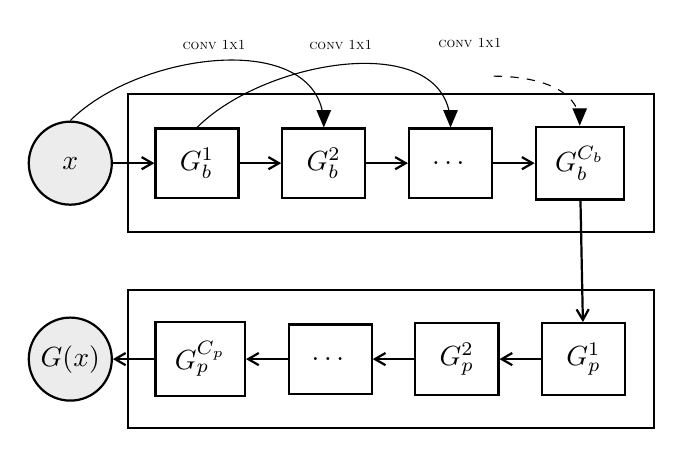
\begin{tikzpicture}
\node[io] (x) {$x$};
\node[group, minimum height=2.5em, minimum width=3em, right=1.5em of x] (b1) {$G_b^1$};
\node[group, minimum height = 5em, minimum width = 19em, right = 0.5em of x] (basestack) {};
\node[group, minimum height=2.5em, minimum width=3em, right=1.5em of b1] (b2) {$G_b^2$};
\node[group, minimum height=2.5em, minimum width=3em, right=1.5em of b2] (bdots) {\dots};
\node[above=1.5em of bdots] (invi2) {};
\node[right=0.5em of invi2] (invi) {};
\node[group, minimum height=2.5em, minimum width=3em, right=1.5em of bdots] (bc) {$G_b^{C_b}$};
\node[io, below=4em of x] (psix) {$G(x)$};
\node[group, minimum height = 5em, minimum width = 19em, right = 0.5em of psix] (specstack) {};
\node[group, minimum height=2.5em, minimum width=3em, right=1.5em of psix] (pc) {$G_p^{C_p}$};
\node[group, minimum height=2.5em, minimum width=3em, right=1.5em of pc] (pdots) {\dots};
\node[group, minimum height=2.5em, minimum width=3em, right=1.5em of pdots] (p2) {$G_p^{2}$};
\node[group, minimum height=2.5em, minimum width=3em, right=1.5em of p2] (p1) {$G_p^{1}$};
%\node[group2, minimum height=4.5em, minimum width=20em, right=1.1em of x] (bstack) {};
%\node[group2, minimum height=4.5em, minimum width=20em, right=1.1em of psix] (pstack) {};
\draw[conn] (x)--(b1);
\draw[conn] (b1)--(b2);
\draw[conn] (b2)--(bdots);
\draw[conn] (bdots)--(bc);
\draw[->] (x.north) to [out=45,in=90] (b2.north) node[above left=3.5em]{\tiny{\textsc{conv 1x1}}};
\draw[->] (b1.north) to [out=45,in=90] (bdots.north) node[above left=3.5em]{\tiny{\textsc{conv 1x1}}};
\draw[dashed,->] (invi.east) to [out=0,in=90] (bc.north) node[above left=3.5em]{\tiny{\textsc{conv 1x1}}};
\draw[conn] (bc)--(p1);
\draw[conn] (p1)--(p2);
\draw[conn] (p2)--(pdots);
\draw[conn] (pdots)--(pc);
\draw[conn] (pc)--(psix);
\end{tikzpicture}
\caption{Feature mapping induced by the component stacks of our architecture space. Each cell in the base stack receives outputs from two previous cells, whereas each cell in the personalized stack receives outputs from only one previous cell.}
\label{c4-fig:architecture}
\end{figure}

\noindent Our algorithm is then composed of a \emph{federated} phase and an \emph{adaptation} phase. In the \emph{federated} phase, we rewrite the Meta-NAS objective in Eq.~\eqref{metaobj} to reflect our factorized architecture space as:
\begin{eqnarray}
F_\tau(\theta_b, \theta_p) &\triangleq& \frac{1}{n} \sum F_{\tau_i}\left(\theta_b, \theta_p - \lambda\nabla_{\theta_p} F_{\tau_i}(\theta_b, \theta_p)\right) \ .
\end{eqnarray}
We then derive the gradient of this personalized NAS objective in Appendix~\ref{app:nas} and propose using a first-order Taylor approximation to efficiently estimate the Hessian terms that arise in the derivative. Subsequently, in the \emph{adaptation} phase, we fix the learned parameters $\theta_b$ of the base component and proceed to fine-tune the specific component for each task using iterative gradient descent update. That is:
\begin{eqnarray}
\theta^{t+1}_p(\tau_i) &\triangleq& \theta^{t+1}_p(\tau_i) - \lambda \nabla F_{\tau_i}\left(\theta^0_b, \theta^t_p(\tau_i)\right) \ ,
\end{eqnarray}
where $\theta^{t}_p(\tau_i)$ denotes the parameters of the specific component of task $\tau_i$ at the $t^{\text{th}}$ adaptation step and $\theta^{0}_p(\tau_i)$, $\theta^{0}_b$ denote the parameters obtained at the end of the \emph{federated} phase. To complete the specification of our algorithm, we further describe the context-aware mapping functions that generate operator mixing weights in Appendix~\ref{app:nas}.

\section{Results}
We compare against several different architecture search and federated learning benchmarks, such as \textsc{FedDSNAS}~\cite{he2020fednas} and \textsc{FedAvg}~\cite{McMahan17}. All of our empirical studies are conducted on two image
recognition datasets: (a) the CIFAR-10 dataset~\cite{cifar10} which aims to predict image labels from 10 classes
given a train/test set of 50000/10000 colour images of dimension 32 × 32 pixels; and (b) the MNIST
dataset~\cite{lecun2010mnist} which aims to predict handwritten digits (i.e. 0 to 9) given a train/test set of 60000/10000
grayscale images of dimension 28×28 pixels. We compare two variants of our framework, \textsc{CA-FedPNAS} (with context-aware
operation sampler) and \textsc{FedPNAS} (without the operation sampler), against: (a) \textsc{FedAvg} of a
fixed architecture to justify the need for NAS in FL; (b) \textsc{FedDSNAS} - which extends DSNAS
to the FL setting; and finally (c) \textsc{CA-FedDSNAS}, which extends \textsc{FedDSNAS} with our
context-aware sampler.

To demonstrate the performance of \textsc{FedPNAS}, we conduct three empirical studies. First, we design a control experiment to test our framework on heterogeneous tasks and demonstrate the necessity of architecture personalization. We simulate this scenario via applying different transformations to each client dataset. We show that on both datasets, both methods with our context sampler \textsc{CA-FedPNAS} and \textsc{CA-FedDSNAS} converge much faster than
their counterparts without the sampler component. The performance gap is significant on the more difficult \textsc{CIFAR-10} dataset. This shows that the contextual information helps to quickly locate regions of high-performing architectures, especially on
similar inputs.

Second, we investigate the respective performances of \textsc{CA-FedPNAS} and
and \textsc{FedDSNAS} on tasks with varying levels of heterogeneity. We simulate this by using varying the complexity level of data transformations, such as small-angle rotations (easy) or hue jitter/large-angle rotations (hard). We observe that our method CA-FEDPNAS achieves better performance, especially on tasks with higher heterogeneity among clients. This clearly shows the importance of architecture personalization when the training tasks are significantly
different and justifies our research goal.

Finally, we assess the quality of the pre-adaptation architecture distributions
respectively discovered by \textsc{CA-FedPNAS} and \textsc{FedDSNAS}. In particular, we use these learned
distributions to generalize to
completely unseen tasks (i.e., tasks that are not observed in the federated learning phase). To simulate
this scenario, during the evaluation
phase, however, we supply each local client with 2000 test images subjected to completely unseen transformations. \textsc{CA-FedPNAS} outperformed other benchmarks without any further finetuning, and this performance gap significantly increases only with $100$ iterations of retraining. This implies that \textsc{CA-FedPNAS} more accurately captured the broad similarity of the task spectrum and
requires minimal additional information to successfully adapt to unseen tasks.

The details of our empirical study is given in Appendix~\ref{app:nas}. Our work has been published to the New Frontiers in Federated Learning:
Privacy, Fairness, Robustness, Personalization and Data Ownership (NFFL) workshop in the Conference on Neural Information Processing Systems (NeurIPS) 2021.
\label{sec:nas}

\chapter{Other work and future directions}
\label{sec:future}
\label{c6:future}
\section{Other algorithmic selection problems for kernel-based methods}
Orthogonal to the approach presented in this thesis, we have also investigated another algorithmic design problem for GP. The classical GP algorithm~\citep{Rasmussen06} trains and runs in $\mathcal{O}(n^3)$ complexity, where $n$ is the size of the training data. Due to this prohibitively expensive cost, many sparse approximations have been employed to improve the scalability of GP in practical use cases. These methods, which are broadly referred to as \textit{sparse GPs} (SGP), usually focus on optimizing a compact set of inducing data points which serve as sufficient statistics for the training data~\cite{Hoang14,Yarin15,Hensman13}. Nonetheless, there have been little study on how large should this inducing set be for the SGP predictions to closely approximate that of GP. 

We developed a set of conditions for the training data such that the sparse spectrum GP (SSGP) method~\cite{Yarin15}, only need a compact inducing set (i.e., the set of spectral frequencies) to closely approximate GP prediction. This is the first theoretical study regarding the approximation quality of SSGP. Based on this theoretical understanding, we further develop a practical approach to \textit{recondition} the training data using a variational autoencoder (VAE) approach~\cite{Kingma13}. We showed that our VAE-transformed data exhibit the proposed conditions and achieve better sample complexity than vanilla SSGP. Our analysis and method has been published at the Conference on Neural Information Processing Systems (NeurIPS) 2020~\cite{hoang2020revisiting}.

In addition, previous chapters have considered both architecture design for Artificial neural networks (ANN) and kernel design for Gaussian processes (GP). Recent work has shown that ANNs are equivalent to GP in the infinite-width limit, and that the evolution of an ANN during training can also be described by a neural tangent kernel (NTK)~\cite{jacot2018neural}. This provides a theoretical connection between two major domains of AAD and reveals a future direction on an unification approach for algorithmic design. 

\section{Designing sequence sketches beyond the minimizer method}
In Chapter~\ref{c4:minimizer}, we have considered the sketch design problem grounded in the minimizer~\citep{schleimer03,marcais17} approach. This has been extended to unify the syncmer approach~\citep{edgar2021syncmers,shaw2021theory} under the masked minimizers method, which is currently being peer reviewed for the conference on Research in Computational Molecular Biology (RECOMB) 2023~\cite{hoang2022masked}. In the remaining timeline of this dissertation, we will continue to investigate other algorithmic design problems in the sequence sketching domain. One example of such problems including configuring the local scheme~\cite{marcais18}, which employs a local $k$-mer ordering per $(w,k)$-window instead of a global ordering as in the minimizer approach. Alternatively, we also consider going beyond the $k$-mer sampling constraint, i.e., can we sketch the sequence using variable-sized substrings or continuous embedding that allows recovery of the original sequence?

\section{Evolution-based meta learning for heterogeneous multi-task AAD}
\label{c5:future}
In Chapter~\ref{c5:nas}, we have considered the multi-task AAD scenario grounded in the Federated NAS problem. We showed that the meta-learning paradigm can be naturally extended to solve AAD optimization tasks with several practical improvements. However, this approach relies on the assumption that all tasks sampled from the given task distribution must be sufficiently similar, such that a single base model can be quickly adapted to solve each of them. In practice, such an assumption is often inappropriate given a long-tailed or multi-modal task distribution. In fact, high task diversity/heterogeneity has been shown to limit the performance of meta learning. For example, \citet{chen2021hetmaml,iwata2020meta}~have recently shown that standard meta learning is not effective on tasks with different feature spaces.

To address this problem, existing approaches~\cite{chen2021hetmaml,iwata2020meta} employ various task embedding strategies to implicitly cluster sampled tasks into different localities of the task manifold. These task embedding modules, however, are solely learned from the sampled task data and are assumed to stay static throughout the meta learning step, hence do not account for subsequent updates of the meta model hypothesis. We instead argue that an accurate task clustering scheme must also account for the underlying function that generates the data, and therefore needs to be concurrently updated together with the learning model.

In the remaining timeline of this thesis, we will investigate a new approach to address this learning scenario. Our preliminary idea is to adopt an evolving ensemble of meta-models to accurately reflect the multi-modality of the task landscape. Each meta model in the ensemble represents a prototype that implicitly defines a cluster of tasks. Cluster membership is then assigned based on a fitness metric that measures task similarity without learning an embedding. In particular, our fitness metric $F(\mathcal{T}, \mathcal{P})$ between a new task $\mathcal{T}$ and a prototype $\mathcal{P}$ will directly measure the agreement between the objective gradients of $\mathcal{T}$ and that of the previous tasks used to update $\mathcal{P}$. Intuitively, we hypothesize that $\mathcal{P}$ is fit to solve $\mathcal{T}$ when all gradients point in a similar direction, and is unfit otherwise. This fitness measures will determine which meta model will get to update with respect to an incoming batch of tasks. We also plan to devise a new evolutionary mechanism to replace obsolete meta models in the ensemble. Explicitly, analogous to a cross-over operator in evolutionary optimization, we will let meta models that are not frequently matched to new tasks distill knowledge from more successful models in the ensemble.

\section{Thesis timeline}
\begin{table}[ht]
\centering
\begin{tabular}{l|l}
\textbf{Timeline}                     & \textbf{Milestones}                                      \\
\hline
November 2022               & Proposal Submission                            \\
November 2022 - January 2023          & Revise Chapter~\ref{c4:minimizer} based on conference review    \\
December - January 2022       & Proposal Presentation                          \\
November 2022 - February 2023  & Conducting research direction proposed in Section~\ref{c5:future}                \\
February 2023 & Submit research work to peer-review conference \\
February 2023 - May 2023     & Thesis writing                                 \\
Apr 2023 - May 2023          & Revise chapter~\ref{c5:nas} based on conference review    \\
June 2023 - July 2023         & Thesis submission/defense   \\
\hline
\end{tabular}
\caption{Proposed timeline of thesis}
\end{table}

% \chapter{Conclusion}
% \label{sec:conclusion}
% \input{conclusion.tex}

\appendix
\section{Details of benchmark sequences}
\label{app-mask:d}
\newcolumntype{D}{>{\centering\arraybackslash}p{13.2cm}}
\setlength{\tabcolsep}{12pt}
\begin{table}[h]
\begin{center}
\begin{tabular}{lll} 
    \toprule
    Label & Description (Assembly) & Length \\
    \midrule
    \textsc{ChrXC} & Centromere region of human chromosome X \cite{miga19} & 3106132 \\ 
    \textsc{Chr1} & Human chromosome 1 & 233587144 \\ 
    \textsc{Btr1} & Blautia producta (GCA\_004210255.1) & 6354838 \\ 
    \textsc{Btr2} & Blautia hansenii DSM 20583 (GCF\_002222595.2) & 3065949 \\ 
    \textsc{Btr3} & [Clostridium] scindens (GCA\_009684695.1) & 3785527 \\ 
    \textsc{Btr4} & Blautia producta ATCC 27340 = DSM 2950 (GCA\_010669205.1) & 6197116 \\ 
    \bottomrule
\end{tabular}
\end{center}
\caption{Descriptions and lengths of sequences used in Section~\ref{sec:result}.}
\label{table:4}
\end{table}

\section{Other implementation details}
\label{app-mask:e}
We implement our method using PyTorch and deploy all experiments on a
RTX-3080 GPU. Due to limited GPU memory, each training epoch only computes the loss on a randomly sampled batch of $32$ substrings of length $\ell = 1500$ bases. The conservation component of $\mathcal{L}_{gss}$ is averaged over $5$ random mutations, simulated using a $10\%$ base substitution rate. Evaluation of conservation is likewise obtained using $5$ random mutations. Network weights are optimized using the ADAM optimizer \cite{kingma14adam} with default parameters.

\section{Other results}
\label{app-mask:f}
\subsubsection{Effectiveness of training on conservation and density metrics.} Fig.~\ref{fig:5} demonstrates the individual effect of training the proposed loss $\mathcal{L}_{gss}$ on the conservation and density metrics. We observe that both conservation and density of the syncmer mask are upper-bounded by that of the minimizer mask, which confirms the result of  Theorem~\ref{theo:1}. We observe that $\mathcal{L}_{gss}$ improves conservation but worsens density for the syncmer mask, which is similar to our first experiment. However, this is not the case for the minimizer and complement mask, which obtain significant improvements in both metrics over $600$ training epochs. We note that this does not contradict our analysis, as conservation is still bounded by density at any point during the training. Rather, this implies that our method has found a favorable trade-off between the two metrics, which in turn explains the sharper increases in GSS compared to that of syncmer across all experiments.

\begin{figure}[ht]
\centering
\begin{tabular}{cc}
\includegraphics[scale=1]{masked_mnz_plots/fig5/compare_con_vs_epoch_chrXC.pdf} & 
\includegraphics[scale=1]{masked_mnz_plots/fig5/compare_den_vs_epoch_chrXC.pdf} \end{tabular}  
\caption{Comparing conservation and density metrics of different masked minimizers vs.\@ number of training epochs on \textsc{ChrXC} with $w=15$ and $k\in\{25,40,55,70\}$.}
\label{fig:5}
\end{figure}

\subsubsection{GSS profiles of minimizer masks on other bacterial genomes.} Fig.~\ref{fig:4b} shows the scatter plots of all $2^w$ masked minimizers trained on \textsc{Btr1}, \textsc{Btr2} and \textsc{Btr3} using $\mathcal{L}_{gss}$ with $w=10$ and $k=15$, grouped by the number of $1$-entries in their masks. We observe the same increasing pattern of average GSS with respect to number of $1$-entries in the mask, thus confirming that the minimizer mask is indeed a good default choice.

\begin{figure}[ht]
\centering
\begin{tabular}{c}
\hspace{-3mm}\includegraphics[scale=0.78]{masked_mnz_plots/fig4/exp7b.pdf}
\end{tabular}
\caption{GSS vs.\@ number of $1$-entries of all mask minimizers on bacterial genomes \textsc{Btr1-3}.}
\label{fig:4b}
\end{figure}

\subsubsection{Exploiting the relative conservation metric with varying offsets.} We repeat this experiment for different syncmer masks with $t\in\{6,7,8,9\}$ and plot all results in Fig.~\ref{fig:6}. In all of these experiments, we observe that the model trained with $n=20$ sampled mutations per epoch always find the exploit within $1000-1500$ epochs. The bar plots once again confirm that for each value of $t$, the exploitative solution contains no segment with more than $t-1$ consecutively decreasing scores. We note that the total count for $t=7$ is significantly lower than other values of $t$ because the solution contains several segments of monotonically increasing scores that are relatively long, which count towards the $>6$ bucket.

\begin{figure}[ht]
\centering
\begin{tabular}{c}
\includegraphics[scale=1.075]{masked_mnz_plots/fig6/exploit_t6.pdf} \\
\includegraphics[scale=1.075]{masked_mnz_plots/fig6/exploit_t7.pdf} \\
\includegraphics[scale=1.075]{masked_mnz_plots/fig6/exploit_t8.pdf} \\
\includegraphics[scale=1.075]{masked_mnz_plots/fig6/exploit_t9.pdf} \\
\end{tabular}
\caption{Finding the relative conservation exploit for various syncmer masks with (from top to bottom) offset $t \in \{6,7,8,9\}$ with $\mathcal{L}_{exploit}$, $w=10$ and $k=15$.}
\label{fig:6}
\end{figure}
\chapter{Kernel Selection Appendix}
\label{app:ks}
\section{Bayesian Generative Search}
\label{app-ks-sec:method}
Similar to~\citet{Lu18}, we reformulate the discrete optimization problem as a BO task over a latent representation space, which allows us to bypass both the need to select an initial set of active candidates~\cite{Duvenaud13} and to rely on heuristic methods for exploring new candidates~\cite{Malkomes16}. However, instead of learning a direct embedding, we implicitly encode composite kernels as output of a parameterized \emph{open-ended recurrent generator}. While~\citet{Lu18} focuses on learning a mapping between latent representations and kernel expressions, our method, \textsc{DTerGenS}, learns a mapping between the latent coordinates and the \emph{infinitely long} kernel expression generative trajectories. This main difference helps to avoid placing an explicit upper limit on the expression length, thus ensuring sufficient expressiveness of the candidate set. 

\begin{figure}
\centering
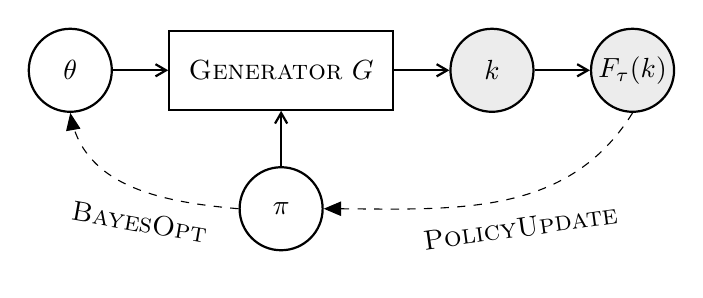
\begin{tikzpicture}
  \node[group2, minimum size=1cm] (g) {\textsc{Generator} $G$};
  \node[neuron, left=2em of g] (t) {$\theta$};
  \node[neuron, below=2em of g] (p) {$\pi$};
  \node[io, right=2em of g] (k) {$k$};
  \node[io, right=2em of k] (f) {$F_{\tau}(k)$};
  \draw[conn] (t) -- (g);
  \draw[conn] (p) -- (g);
  \draw[conn] (g) -- (k);
  \draw[conn] (k) -- (f);
  \draw [dashed,->] (f.south) to [out=-122,in=0] (p.east) node[below right=1.2em, rotate=8]{\ \ \ \ \ \ \ \textsc{PolicyUpdate}};
  \draw [dashed,->] (p.west) node[below left=0.5em, rotate=-10]{\textsc{BayesOpt}\ \ } to [out=-185,in=-80] (t.south);
\end{tikzpicture}
\caption{The generic workflow of \textsc{DTerGenS}. Given policy $\pi$, we employ BO to obtain generative weight candidate $\theta$ (Section~\ref{app-ks-subsec:theta}). Using the observed generative trajectory, we alternately update the policy distribution (Section~\ref{app-ks-subsec:pi}).}
\label{app-fig:workflow}
\end{figure}

The VAE decoder in~\cite{Lu18}, which sequentially generates the next operand and operator given the current expression, is pre-trained with the VAE encoder using randomly sampled kernel expressions. In contrast, our generator explicitly captures the \emph{sum-of-product} structure through a nested recursion procedure, thus is capable of generalizing the composition rules to create new expressions. To prevent the generation of infinitely long and computationally expensive expressions, we learn a stochastic early stopping policy, which determines the best performing stopping point on any generative trajectory. This method enables the exploration of arbitrarily complex expressions and is the first selection method that places no further structural restriction on the search space.

Both the generative parameters and the termination policy can be jointly optimized by exploiting their dynamic in the generative component. Fixing a termination policy, we devise a dynamic BO algorithm for optimizing generative parameters that is capable of adapting to the constant policy updates. Alternately, given each sample trajectory collected by the BO step, we devise an update algorithm for the policy distribution via modelling the dynamic between these two components. Together, these steps compose our main contribution, which is the \textsc{DTerGenS} algorithm for composite kernel selection. 

We demonstrate that \textsc{DTerGenS} is able to produce sophisticated kernel expressions, which significantly improve the predictive performance over state-of-the-art methods on multiple benchmarks. Our results show a wider range of structures being explored by \textsc{DTerGenS} and faster convergence compared to other methods. Finally, we show that \textsc{DTerGenS} is also able to recover known well-performing kernels on artificially designed predictive tasks.

\subsection{Reformulating Kernel Selection}
\label{app-ks-subsec:reformulation}
Directly optimizing over the discrete domain of kernel expressions as suggested by Definition~\ref{c3-def:ksproblem} is challenging. To work around this, we model $k$ as the output of a generative process $G(\theta, \pi)$ conditioned on $\theta$ and $\pi$, which controls the termination of $G$. The designs of $G$ and $\pi$ are given in Section~\ref{app-ks-subsec:generator} and Section~\ref{app-ks-subsec:pi} respectively. We approximate the original kernel selection objective in Definition~\ref{c3-def:ksproblem} as:
\begin{eqnarray}
\underset{k \in \mathcal{K_C}}{\argmax} \ F_{\Omega}(k) &\simeq&  \underset{\theta \in \Theta, \pi \in \Pi}{\argmax} \ R_{\tau} (\theta, \pi) \ ,
\label{app-ks-prop:reformulation}
\end{eqnarray}
where $R_\tau$ is defined as the composite function $F_\tau \circ G$.

\noindent Our framework alternately optimizes each component $\pi$ and $\theta$ while fixing the other as constant. Explicitly, given a policy $\pi$, the generative parameter $\theta$ is optimized using an adapted BO algorithm that is formulated with the conditional policy distribution $p(\pi \mid \theta)$ (Section~\ref{app-ks-subsec:theta}). On the other hand, given the BO-sampled observations, the policy distribution $p(\pi \mid \theta)$ can be updated via MLE (Section~\ref{app-ks-subsec:pi}). The outline of this workflow is illustrated in Fig.~\ref{c3-fig:workflow}. To lay the groundwork for our algorithmic development, we will first discuss the design of our kernel generator $G(\theta, \pi)$ in Section~\ref{app-ks-subsec:generator}.

\subsection{Open-ended Kernel Generator}
\label{app-ks-subsec:generator} 
A composite kernel expression, written as a sum-of-products over base kernel units in Eq.~\eqref{c3-eq:general}, naturally manifests as a tree with (1)~a primary linear chain; and (2)~several secondary linear branches that are connected to the primary chain. The secondary branches denote different products of base kernel units, whereas the primary chain denotes the summation over them. To generate such structures, we construct $G$ by composing two nested recurrent units, which are described below. Fig.~\ref{app-ks-fig:generator} further visualizes the blueprint of this generator architecture.
\subsubsection{Generator Overview}
Our generator architecture comprises of a primary unit and a secondary unit, which respectively generate the primary chain and the secondary branches. Each unit composes of a recurrent neural network (RNN) and a termination policy, which predicts a stopping signal given the hidden state of the neural network. Every recurring step of the primary unit initiates a new secondary branch and computes an initial hidden state for the secondary RNN. On the other hand, every recurring step of the secondary unit generates a new base kernel unit on the current branch. Each unit will recur until its respective policy outputs a stopping signal given the respective current hidden state. When the primary unit terminates, we output a tree structure corresponding to a composite kernel. We give the mechanism of each component below.
\begin{figure}[t]
\centering
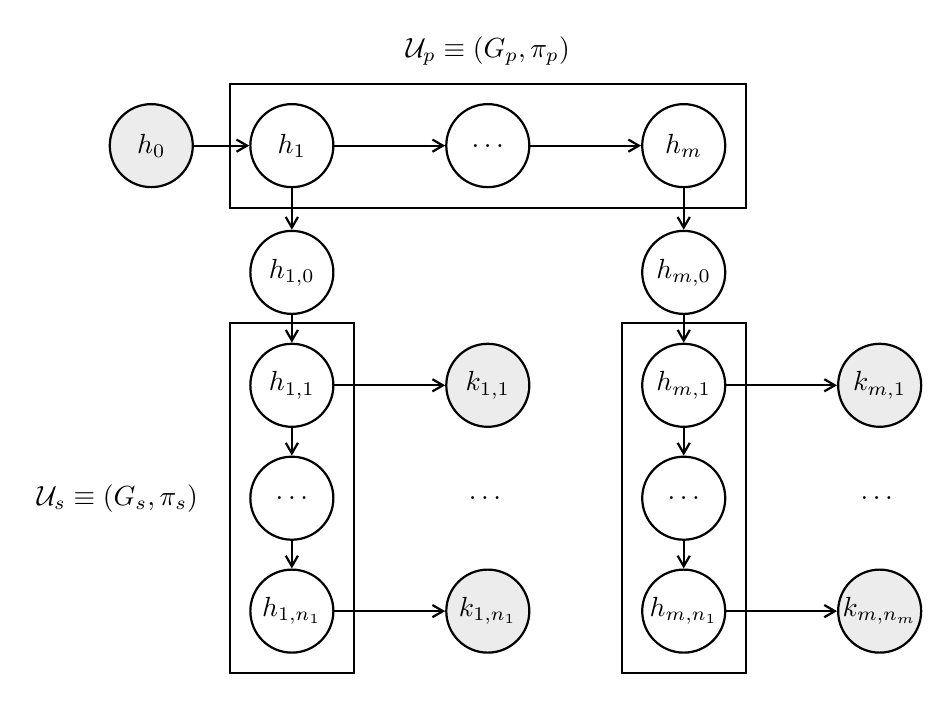
\begin{tikzpicture}
  \node[io] (x0) {$h_0$};
  \node[neuron,right=of x0] (x1)
  {$h_{1}$};
  \node[neuron,right=4em of x1] (dot)
  {$\ldots$}; 
  \node[neuron,right=4em of dot] (xM)
  {$h_{m}$};
  
  \node[neuron,below=1.5em of x1] (x1_0)
  {$h_{1,0}$};
  \node[neuron,below=1em of x1_0] (x1_1)
  {$h_{1,1}$};
  \node[neuron,below=1em of x1_1] (dot2)
  {$\ldots$};
  \node[right=4.5em of dot2] (dot3)
  {$\ldots$}; 
  \node[io,right=4em of x1_1] (o1_1)
  {$k_{1,1}$};
  \node[neuron,below=1em of dot2] (x1_N)
  {$h_{1, n_1}$};
  \node[io,right=4em of x1_N] (o1_N)
  {$k_{1, n_1}$};
  
  \node[neuron,below=1.5em of xM] (xM_0)
  {$h_{m,0}$};
  \node[neuron,below=1em of xM_0] (xM_1)
  {$h_{m,1}$};
  \node[neuron,below=1em of xM_1] (dot4)
  {$\ldots$};
  \node[right=4.5em of dot4] (dot5)
  {$\ldots$}; 
  \node[io,right=4em of xM_1] (oM_1)
  {$k_{m,1}$};
  \node[neuron,below=1em of dot4] (xM_N)
  {$h_{m, n_1}$};
  \node[io,right=4em of xM_N] (oM_N)
  {$k_{m, n_m}$};
  
  \node[left=1.5em of dot2] (gs)
  {$\mathcal{U}_s \equiv (G_s, \pi_s)$};
  \node[above=1em of dot] (gp)
  {$\mathcal{U}_p \equiv (G_p, \pi_p)$};
  \node[group,fit={(x1) (dot) (xM)}] (gr1) {};
  \node[group,fit={(x1_1) (dot2) (x1_N)}] (gr2) {};
  \node[group,fit={(xM_1) (dot4) (xM_N)}] (gr3) {};
  \draw[conn] (x0) -- (x1);
  \draw[conn] (x1) -- (dot);
  \draw[conn] (dot) -- (xM);
  
  \draw[conn] (x1) -- (x1_0);
  \draw[conn] (x1_0) -- (x1_1);
  \draw[conn] (x1_1) -- (dot2);
  \draw[conn] (dot2) -- (x1_N);
  \draw[conn] (x1_1) -- (o1_1);
  \draw[conn] (x1_N) -- (o1_N);
  
  \draw[conn] (xM) -- (xM_0);
  \draw[conn] (xM_0) -- (xM_1);
  \draw[conn] (xM_1) -- (dot4);
  \draw[conn] (dot4) -- (xM_N);
  \draw[conn] (xM_1) -- (oM_1);
  \draw[conn] (xM_N) -- (oM_N);
\end{tikzpicture}
\caption{Schematic of the kernel generator with nested units $\mathcal{U}_p$ and $\mathcal{U}_s$. Each component recursively computes its next hidden state and emission output using respective recurrent neural network $G_s$ and $G_p$. The termination probability at each generative step is determined by policies $\pi_p$ and $\pi_s$. The final candidate kernel expression is composed using Eq.~\eqref{c3-eq:general}.}
\label{app-ks-fig:generator}
\end{figure}
\subsubsection{Primary Unit}
The primary unit $\mathcal{U}_p: \mathbb{R}^{d_p} \rightarrow \mathcal{K_C}$ is given by the RNN $G_p$ and the policy $\pi_p: \mathcal{K_C} \rightarrow \mathbb{R}$. $G_p$ has hidden dimension $d_p$ and emits an initial hidden state for $G_s$. Given an arbitrary initial hidden state $h_0 \in \mathbb{R}^{h_p}$, $G_p$ performs the following at any generative step $t \geq 0$:
\begin{itemize}
\item If $t=0$, initialize candidate kernel expression $\bar{k} = 0$ (i.e., a constant function).
\item Generate the next hidden state and the current emission output: $(h_{t+1}, h_{t,0}) \leftarrow G_p(h_t; \theta_t)$. 
\item Generate and append the $t^{\text{th}}$ secondary branch to the current expression: $\bar{k} \leftarrow \bar{k} + \mathcal{U}_s(h_{t,0}; \theta_s, \pi_s)$.
\item Query termination probability with the current intermediate expression: $\alpha \leftarrow \pi_p(\bar{k})$. 
\item With probability $\alpha$, end the generative procedure and return $\bar{k}$ as a terminal expression. 
\item With probability $1 - \alpha$, set $t \leftarrow t+1$ and repeat the procedure.
\end{itemize}

\subsubsection{Secondary Unit}
The secondary unit $\mathcal{U}_s: \mathbb{R}^{d_s} \rightarrow \mathcal{K_C}$ is given by the RNN $G_s$ and the policy $\pi_s: \mathcal{K_C} \rightarrow \mathbb{R}$. $G_s$ has hidden dimension $d_s$ and emits one-hot representations of the base kernel units in $\mathcal{K_B}$. Given an initial hidden state $h \in \mathbb{R}^{d_s}$ output by $G_p$, $\mathcal{U}_s$ generates a corresponding product of base kernel units. Given an initial hidden state $h_{t,0}$ produced by $G_p$ at time $t$, $G_s$ then performs the following at any inner loop generative step $t' \geq 0$:
\begin{itemize}
    \item If $t'=0$, initialize the inner loop kernel expression $\bar{k}_t = 1$ (i.e., a constant function).
    \item Generate the next hidden state and emit the current base kernel: $(h_{t, t'+1}, k_{t, t'})~\leftarrow~G_s(h_{t, t'}; \theta_s)$.
    \item Extend current expression via multiplication: $\bar{k}_t = \bar{k}_t \times k_{t, t'}$.
    \item Query the termination probability $\beta \leftarrow \pi_s(\bar{k} + \bar{k}_t)$.
    \item With probability $\beta$, end the generative procedure for the current branch and return $\bar{k}_t$.
    \item With probability $1 - \beta$, set $t' \leftarrow t' + 1$ and repeat the procedure.
\end{itemize}
\subsubsection{Termination Policy}
Let $\tau = \{\mathbf{x}_1, \mathbf{x}_2 \ldots \mathbf{x}_n\}$ denote the set of training inputs specified by the learning instance $\Omega$, as introduced in Definition~\ref{c3-def:ksproblem}. The termination policies $\pi_p$ and $\pi_s$, respectively parameterized by the neural networks $\gamma_p$ and $\gamma_s$, are given as follows:
\begin{eqnarray}
\pi_p(k; \gamma_p, \tau) &\triangleq& \sigma\left(\sum_{i,j\in[n]}\gamma_p(\mathbf{x}_i)\cdot\gamma_p(\mathbf{x}_j)\cdot k(\mathbf{x}_i,\mathbf{x}_j)\right)\nonumber \ , \\ 
\text{and} \quad \pi_s(k; \gamma_s, \tau) &\triangleq& \sigma\left(\sum_{i,j\in[n]}\gamma_s(\mathbf{x}_i)\cdot\gamma_s(\mathbf{x}_j)\cdot k(\mathbf{x}_i,\mathbf{x}_j)\right) \ ,
\end{eqnarray} 
where $\sigma(t) \triangleq 1/(1 + \mathrm{exp}(-t))$ denotes the sigmoid activation function. This data-driven parameterization serves to model the task-specific termination rules conditioned on observation task data, which implies that different expression lengths are required for different tasks. We further model the interaction between generative weights $\theta$ and termination policies $\pi$ using the conditional distributions $p(\gamma_s \mid \theta)$ and $p(\gamma_p \mid \theta)$, which in turn are used to construct a kernel function (that models the covariance between composite kernels) of an adapted BO routine (Section~\ref{app-ks-subsec:theta}). This allows us to sample policies given a candidate generative weight and distills finite kernel expression from the potentially infinite trajectory. On the other hand, the adapted BO routine will collect the full trajectory of kernel generation per iteration (consisting of all intermediate expressions until the termination point). This is then used to optimize the above conditional distribution via minimizing a heuristic loss function, thus allowing us to alternately learn the dynamics between $\theta$ and $\pi$ (Section~\ref{app-ks-subsec:pi}).

\subsection{Generative Parameter Optimization}
\label{app-ks-subsec:theta}
% \begin{algorithm}[tb]
%   \caption{\textsc{DTerGenS} - Kernel Selection}
%   \label{alg.dtergens}
% \begin{algorithmic}[1]
%   \STATE {\bfseries Input:}  $\mathcal{F}_\Omega$, $n_{\mathrm{BO}}$, $\gamma = \{n_w, n_\epsilon, n_\ell, \lambda_p, \lambda_s\}$
%   \STATE $\mathcal{G} \leftarrow$ \textsc{CreateGenerator}
%   \STATE $\eta_p,\eta_s \leftarrow$ \textsc{InitializePolicy}
%   \FOR{$t=1$ {\bfseries to} $n_{\mathrm{BO}}$}
%   \STATE $\theta^t \leftarrow {\mathrm{argmax}}_\theta\ f_{\mathrm{acq}}(\theta)$
%   \STATE \textsc{Sample} $\pi_p \sim p(\pi_p \mid \theta^t_p)$
%   \STATE \textsc{Sample} $\pi_s \sim p(\pi_s \mid \theta^t_s)$
%   \STATE $\mathbf{k}_t \leftarrow \mathcal{G}(\theta^t, \pi_p, \pi_s)$
%   \STATE $\mathbf{k}^\ast \leftarrow \mathrm{argmax}_{\mathbf{k} \ \subseteq_{\mathcal{K}}\mathbf{k}_t} \ \mathcal{F}_\Omega(\mathbf{k})$
%   \STATE \textsc{PolicyUpdate}$(\mathbf{k}^\ast,\theta^t,\gamma)$
%   \STATE \textsc{BayesianUpdate}$\left(\theta^t, \mathcal{F}_\Omega(\theta^t), p(\pi_p|\theta^t_p),p(\pi_s|\theta^t_s)\right)$
%   \ENDFOR
% \end{algorithmic}
% \end{algorithm}

In this section, we detail our BO algorithm to optimize the generative weight $\theta$. Formally, fixing a policy distribution $\bar{\pi}$ whose parameterization $\bar{\gamma}$ follows the conditional distribution $\bar{p}(\gamma \mid \theta) \triangleq \bar{p}(\gamma_p \mid \theta)\bar{p}(\gamma_s \mid \theta)$, the partial objective can be rewritten as:
\begin{eqnarray}
\theta^\ast \ = \ \underset{\theta\in\Theta}{\argmax} \  g_{\bar{\pi}}(\theta) & \equiv & \underset{\theta \in \Theta}{\argmax} \ \mathbb{E}_{\gamma \sim \bar{p}}\left[ R_\tau(\theta, \pi(\gamma))\right] \ .
\end{eqnarray}
We then adopt the standard practice of BO~\cite{Snoek12} and impose a Gaussian Process (GP)~\cite{Rasmussen06} prior on the black-box function $g_{\bar{\pi}}$, i.e., $g_{\bar{\pi}} \sim \mathcal{GP}(\mu, k_{\mathrm{BO}})$ where $\mu$ and $k_{\mathrm{BO}}$ respectively denote its mean and covariance functions. The BO algorithm iteratively obtains the next best candidate $\theta$ by maximizing a surrogate acquisition function constructed from the posterior distribution of this GP. The black-box evaluation $g_\pi(\theta)$ is then used to update the GP posterior.

Note that in standard BO setting, the functional landscape is static, whereas in our formulation $\bar{\pi}$ is alternately optimized after every BO iteration, which results in a changing function $g_{\bar{\pi}}$. To account for this dynamic update of ${\bar{\pi}}$, we will therefore model the GP covariance using two components: (1)~an intrinsic kernel component that characterizes the feature distance between the generative weights $\theta_i$ and $\theta_j$; and (2)~an extrinsic kernel component that captures the divergence of their conditional policy distribution $p(\gamma \mid \theta_i)$ and $p(\gamma \mid \theta_j)$ given the current parameterization $\gamma_p$, $\gamma_s$. Explicitly, given candidates $\theta_i$ and $\theta_j$, the kernel distance between these candidates is given as:
\begin{eqnarray}
k_{\mathrm{BO}}(\theta_i, \theta_j) &\triangleq& k_{\textsc{Policy}}(\theta_i, \theta_j)\cdot k_{\textsc{Generator}}(\theta_i, \theta_j) \ ,
\end{eqnarray}
where $k_{\textsc{Generator}}$ is given by the standard squared exponential kernel and $k_{\textsc{Policy}}$ is given by the symmetric KL divergence between the policy distributions conditioned on $\theta_i$ and $\theta_j$ respectively:
\begin{eqnarray}
k_{\textsc{Policy}}(\theta_i, \theta_j) &\triangleq& \mathbb{KL}\Big(p(\gamma\mid\theta_i) \ \| \ p(\gamma \mid\theta_j)\Big)  \ .
\end{eqnarray}

\subsection{Optimizing Policy Distribution}
\label{app-ks-subsec:pi}
We use the same notation $\gamma$ to refer to both policy $\gamma_p$ and $\gamma_s$ in this section due to their symmetry. We first give our parameterization for the policy distribution $p(\gamma \mid \theta)$ using a standard Bayesian neural networks:
\begin{eqnarray}
p(\gamma \mid \theta) &\sim& \mathcal{N}(\gamma_p; \mu(\theta), \Sigma(\theta)) \ ,
\end{eqnarray}
where $\mu$ and $\Sigma$ are deep neural networks that respectively generate the mean and covariance of the distribution. This section then details an update iteration of $\mu$ and $\sigma$ given a new candidate weight $\theta$ (derived from maximizing the BO acquisition function) and its corresponding kernel expression $k = \sum_{t=1}^m\prod_{t'=1}^{n_t} k_{t, t'}$ where $k_{t, t'} \in \mathcal{K_B}$. Since the generative trajectory encoded by $\theta$ is infinite, there is no analytical method to compute its optimal set of stopping points. However, we can approximate the optimal stopping point in this trajectory by finding the best performing intermediate kernel expression on the observed finite trajectory. Explicitly, let $\mathcal{S} = \{\{\bar{m}, \bar{n}_1, \bar{n}_2 \dots \bar{n}_m\} \mid \bar{m} \leq m, \forall t \in [\bar{m}]: \ \bar{n}_t \leq n_t\}$ be the set of all possible intermediate sets of stopping points that precede $k$, we define the \emph{hindsight estimation} of $k$ as:

\begin{eqnarray}
k^\ast &=& \sum_{t=1}^{m^\ast}\prod_{t'=1}^{n^{\ast}_{t}} k_{t, t'}, \quad \text{where} \nonumber \\
\{m^\ast, n^\ast_1 \dots n^\ast_{m^{\ast}}\} &\triangleq& \underset{
 \{m', n'_1, \dots n'_m\} \in \mathcal{S}
}{\argmax} F_{\tau}\left(\sum_{t=1}^{m'}\prod_{t'=1}^{n'_{t}} k_{t, t'}\right) \ ,
\end{eqnarray}
and let $K^\ast_{\tau}$ denote the covariance matrix induced by $k^\ast$ on training inputs the ${\mathcal{D}}$ described in $\tau$. We argue that high-performing kernels likely produce covariance matrices that are similar to $K^\ast_{\tau}$ , which motivates the following loss function with respect to current candidate weight $\theta$ :
\begin{eqnarray}
\mathcal{L}_\theta(\mu, \sigma) &=& \mathbb{E}_{\gamma\sim \mathcal{N}(\mu(\theta), \sigma(\theta))}\Big[ \left\langle{G}(\theta, \pi(\gamma)),k^\ast\right\rangle_{\tau}\Big] \nonumber \\
&\simeq& \frac{1}{r_{\gamma}}\sum_{i=1}^{r_{\gamma}} \left\langle{G}(\theta, \pi(\gamma_i)),k^\ast\right\rangle_{\tau}
\end{eqnarray}
where $r_\gamma$ denotes the number of $\gamma$ samples drawn from the conditional distribution; $\pi(\gamma_i)$ denotes the termination policy parameterized by $\gamma_i$ drawn from the conditional policy distribution; $G(\theta, \pi(\gamma_i))$ denotes the kernel expression generated by $G$ with weight $\theta$ and policy $\pi(\gamma_i))$; and $\langle k, k'\rangle_{\tau} \triangleq \|K_{\tau}-K'_{\tau}\|_{\mathrm{Fro}}$ denotes the Frobenius norm of the difference between the covariance matrices induced by kernel functions $k$ and $k'$. This loss function, however, does not have an analytical gradient with respect to $\mu$ and $\sigma$ as it requires simulation to compute. To optimize for $\mu$ and $\sigma$, we first employ the random gradient estimation technique~\cite{nesterov17}, which approximates gradient at a point by evaluating the expected gradient of its $\upsilon$-Gaussian smoothing. In particular, we derive our randomized gradient estimation for $\mu$ as follows:
\begin{eqnarray}
\nabla_{\mu} \mathcal{L}_\theta(\mu, \sigma) &\simeq& \nabla_\mu \  \mathbb{E}_{\upsilon\sim\mathcal{N}(0, \mathbf{I})}\left[\ell_\theta(\mu + \upsilon, \sigma)\right] \nonumber \\
&=& \mathbb{E}_{\upsilon\sim\mathcal{N}(0, \mathbf{I})}\left[\ell_\theta(\mu + \upsilon, \sigma)\upsilon\right] \nonumber \\
&\simeq& \frac{1}{r_\upsilon} \sum_{j=1}^{r_\upsilon} \ell_\theta(\mu + \upsilon_j, \sigma)\upsilon_j \nonumber
\\ 
&\simeq& \frac{1}{r_\gamma r_\upsilon} \sum_{i=1}^{r_\gamma}\sum_{j=1}^{r_\upsilon} \left\langle G(\theta, \pi(\mu_i + \upsilon_j, \sigma_i), k^{\ast} \right\rangle_{\tau} \ ,
\end{eqnarray}
where $r_\upsilon$ denotes the number of $\upsilon$ samples drawn from the standard Gaussian distribution $\mathcal{N}(0, \mathbf{I})$ and we have rewritten $\pi(\gamma_i) = \pi(\mu_i, \sigma_i)$ to clearly show the perturbed component $\mu_i$ in the estimation. Similarly, the gradient estimation for $\sigma$ is given as:
\begin{eqnarray}
\nabla_{\sigma} \mathcal{L}_\theta(\mu, \sigma) &\simeq& \frac{1}{r_\gamma r_\upsilon} \sum_{i=1}^{r_\gamma}\sum_{j=1}^{r_\upsilon} \left\langle G(\theta, \pi(\mu_i, \sigma_i + \upsilon_j), k^{\ast} \right\rangle_{\tau} \ .
\end{eqnarray}
These estimations allow us to update $\mu$ and $\sigma$ via the gradient descent algorithm, which complete the specification of our policy update. 

\section{Experiments}
\label{app-ks-sec:exp}
This section evaluates and reports the empirical performance of our kernel selection framework $\textsc{DTerGenS}$ on a synthetic kernel recovery task and kernel selection for regression on three real-world datasets:
\begin{itemize}
\item The DIABETES dataset~\cite{UCI_diabetes_data} contains 442 diabetes patient records (i.e., inputs) with 10 variables: age, sex, body mass index, average blood pressure and six blood serum measurements. The target output variable is a quantitative measure of disease progression one year after baseline.
\item The MAUNA LOA dataset~\cite{mauna_loa_data} measures monthly average $\mathrm{CO}_2$ concentration (in ppvm) of air samples at the Mauna Loa Observatory over 42 years (i.e., 504 observations in total).
\item The PROTEIN dataset~\cite{UCI_protein_data} features 45730 observations of protein tertiary structures, each records 9 physicochemical properties of a protein. The target output variable is the size of the protein residue in kDa.
\end{itemize}
To demonstrate the performance of \textsc{DTerGenS}, we compare our method with the following benchmarks: (a) random search over the space of kernels with max length $L \leq 10$ (baseline); (b) \textsc{SVO}: Structure Variationally-Encoded Optimization~\cite{Lu18}, for which we train the VAE component using 25000 randomly generated kernel expressions with max length $L \leq 10$ (to show the advantage of generative search); and (c) our own algorithm with no stopping policy and fixing expression length $L = 2, 4, 8$. For (c), the termination of the secondary component is chosen at random, the termination of primary component is guaranteed upon reaching length $L$, and REMBO~\cite{Wang16} is used to optimize generative weights $\theta$. This setting is meant to demonstrate the advantage of having adaptive termination policies for the generative components. 

For all experiments, we demonstrate the performance of our framework on the black-box model Variational DTC Sparse Gaussian Process (vDTC)~\cite{Hensman13} with the following configurations: (1) 80/10/10 train-test-validation split (i.e., we use the validation fold to compute BO feedback and the test fold to evaluate final performance); (2) 100 randomly selected inducing inputs; (3) kernel hyper-parameters are optimized using L-BFGS over 100 iterations. These configurations implicitly define the learning scenario $\Omega$, such that $F_{\Omega}$ is the root-mean-square-error (RMSE) of predictions on the test split, given a model trained and validated accordingly on the train split. We construct the set of base kernels with $4$ different base kernel functions, as suggested by~\citet{Duvenaud13}. These kernel functions, along with their learnable parameters, are defined as follows:
\begin{eqnarray}
k_{\mathrm{LIN}}(\mathbf{x}_i, \mathbf{x}_j; \sigma_n, \sigma_b, \mathbf{c}) &\triangleq& \sigma_n^2 \left(\mathbf{x}_i - \mathbf{c}\right)^\top\left(\mathbf{x}_j - \mathbf{c}\right) + \sigma_b^2 \\
k_{\mathrm{SE}}(\mathbf{x}_i, \mathbf{x}_j; \sigma_n, \ell_1, \ell_2 \dots \ell_d) &\triangleq& \frac{1}{\sigma^2_n} \exp \left(\sum_{t=1}^d \frac{(\mathbf{x}^t_i - \mathbf{x}^t_j)^2}{\ell_t^2}\right) \\
k_{\mathrm{PER}}(\mathbf{x}_i, \mathbf{x}_j; \sigma_n, \sigma_p, \ell_1, \ell_2 \dots \ell_d) &\triangleq& \frac{1}{\sigma^2_n} \exp \left(\sum_{t=1}^d \frac{2\sin^2\left(\pi|\mathbf{x}^t_i - \mathbf{x}^t_j|/\sigma_p\right)}{\ell_t^2}\right) \\
k_{\mathrm{RQ}}(\mathbf{x}_i, \mathbf{x}_j; \sigma_n, \sigma_w, \mathbf{c}) &\triangleq& \sigma_n^2 \left(1 + \sum_{t=1}^d \frac{(\mathbf{x}^t_i - \mathbf{x}^t_j)^2}{2\sigma_w^2\ell^2_t}\right)^{-\sigma_w}
\end{eqnarray}

\noindent We parameterize $G_p$ and $G_s$ using the same RNN architecture with 4 hidden feed-forward layers. Both $G_p$ and $G_s$ has hidden dimension $d_p = d_s = 5$. The emission output of $G_p$ has dimension $d_s=5$, as $G_p$ is tasked to generate the initial hidden state of $G_s$, whereas the emission output of $G_s$ has dimension $|\mathcal{K_B}|=4$, which corresponds to the number of base kernel functions. We use ReLU activation for all non-output layers, softmax activation for the kernel output layer of $G_s$ and tanh activation for the emission output layer of $G_p$. Finally, we optimize our RNN parameters by adapting a known high-dimensional BO method called REMBO~\cite{Wang16} to account for the dynamic function landscape (Section~\ref{app-ks-subsec:theta}). 
\subsection{Synthetic Kernel Recovery}
\begin{figure}
\centering
\begin{tabular}{cc}
\vspace{-2mm}
\includegraphics[width=0.45\linewidth]{./kernel_plots/synthetic_exp0.png} & \includegraphics[width=0.45\linewidth]{./kernel_plots/diabetes.png} \\ 
\vspace{-1mm}
(L1) $\mathrm{RQ} \times \mathrm{RQ}$ & (R1) DIABETES \\
\includegraphics[width=0.45\linewidth]{./kernel_plots/synthetic_exp1.png} & 
\includegraphics[width=0.45\linewidth]{./kernel_plots/mauna.png} \\ 
\vspace{-2mm}
(L2) $\mathrm{PER} \times \mathrm{RQ} \times \mathrm{LIN} \times \mathrm{LIN}$ & (R2) MAUNA LOA \\
\vspace{-3mm}
\includegraphics[width=0.45\linewidth]{./kernel_plots/synthetic_exp2.png} &
\includegraphics[width=0.45\linewidth]{./kernel_plots/protein.png} \\
\vspace{-3mm}
(L3) $\mathrm{LIN} \times \mathrm{RQ} \times \mathrm{LIN} \ + $ & (R3) PROTEIN \\
$\mathrm{PER} \times \mathrm{LIN} + \mathrm{RQ} \times \mathrm{SE}$ & \\
\end{tabular}
\caption{
(Left): Best kernel recovery error over 100 iterations with various kernel selection methods on three synthetic datasets constructed from specific kernels; (Right):
Best nRMSE over 100 iterations with various kernel selection methods on 3 benchmark datasets using vDTC~\cite{Hensman13}.}
\label{app-ks-fig:recovery}
\end{figure}
We first investigate how well various kernel selection methods recover a covariance matrix given synthetic data randomly drawn from its corresponding distribution. Unlike most real-world settings where a ground truth kernel is not known and performance evaluation relies on possibly noisy predictive accuracy, this scenario provides a ground truth for kernel selection and allows us to directly measure the success of various contending methods.

Explicitly, given an arbitrarily chosen kernel $k^{\ast}$ (with arbitrarily initialized hyper-parameters) and $n$ i.i.d. input observations $\tau = \{\mathbf{x}_1, \mathbf{x}_2 \dots \mathbf{x}_n\} \subset \mathbb{R}^d$ drawn from $\mathcal{N}(\mathbf{0}, \mathbf{I})$, we subsequently generate corresponding output observations $Y = \{y_1, y_2 \dots y_n\}$, where $y_i \sim \mathcal{N}(0, K^{\ast}_\tau + \sigma^2\mathbf{I})$ and $K^{\ast}_\tau$ denotes the data covariance matrix induced by $k^{\ast}$. We then apply various kernel selection methods, including $\textsc{DTerGenS}$ for vDTC prediction on this synthetic dataset and measure our recovery error for any selected kernel $k$ by $\mathcal{L}_{\mathrm{rec}}(k) = \|K_\tau - K^{\ast}_\tau\|_{\mathrm{Fro}}$. Fig.~\ref{app-ks-fig:recovery} (left) shows the best recovery errors achieved over a span of 100 BO iterations with 3 different ground truth kernels: (1) $k^\ast = k_\mathrm{RQ}\times k_\mathrm{RQ}$; (2) $k^\ast = k_\mathrm{PER}\times k_\mathrm{RQ}\times k_\mathrm{LIN}\times k_\mathrm{LIN}$; and (3) $k^\ast = k_\mathrm{LIN}\times k_\mathrm{RQ}\times k_\mathrm{LIN} + k_\mathrm{PER}\times k_\mathrm{LIN} + k_\mathrm{RQ}\times k_\mathrm{SE}$. 
\begin{figure}
\begin{tabular}{cc}
\includegraphics[width=0.48\columnwidth]{./kernel_plots/mauna_visual.png} & \includegraphics[width=0.48\columnwidth]{./kernel_plots/unique_k.png} \\
(a) & (b)
\end{tabular}
\caption{(a) The linear-periodic trend of the MAUNA dataset; and (b) number of unique kernels discovered by \textsc{DTerGenS}, \textsc{SVO} and random search on all three datasets.}
\label{app-ks-fig:visual}
\end{figure}

In all experiments, $\textsc{DTerGenS}$ consistently achieves the lowest recovery error after 100 iterations compared to other methods. Random search performs competitively when the ground truth kernels are simple (i.e., $L=2,4$), hence easy to be found via randomization. On the other hadn, random search expectedly performs the worst when the ground truth kernel is longer (i.e., $L=7$). We also observe that without the termination policy component, the performance of $\textsc{DTerGenS}$ is only competitive when $L$ is set to be roughly the length of the ground truth kernel, but otherwise outperformed by other methods. This shows the importance of adaptively learning the complexity of the kernel expression using a data driven policy. Lastly, we observe that $\textsc{SVO}$ is most significantly outperformed by $\textsc{DTerGenS}$ in the first
experiment. We reason that this is because the number of length-$2$ kernels is relatively smaller in the set of training expressions for the VAE component of $\textsc{SVO}$. Thus, the trained VAE could be biased to produce longer kernels and it is more difficult for $\textsc{SVO}$ to find a latent embedding that decodes to a length-$2$ kernel. In contrast, $\textsc{DTerGenS}$ does not incur this problem because its termination policy is also learned as it collects information about the embedding space.
\subsection{Kernel Selection for Regression Task}
This section investigates the performance of kernel selection for regression tasks using vDTC~\cite{Hensman13} on DIABETES~\cite{UCI_diabetes_data}, MAUNA~\cite{mauna_loa_data} and PROTEIN~\cite{UCI_protein_data} datasets. In all experiments, we measure performance by computing the root-mean-square-error of predictions, normalized against the root-mean-square-error achieved by fixing the kernel of \textsc{vDTC} to be $k_{\mathrm{SE}}$, which serves to demonstrate the improvement over the default choice of kernel. Explicitly, our kernel selection metric for any selected kernel $k$ is given by:
\begin{eqnarray}
\mathrm{nRMSE}(k) &\triangleq& \sqrt{\frac{\sum_{i=1}^{n_{\mathrm{test}}} \left(\bar{y}_i(k) - y_i\right)^2 }{\sum_{i=1}^{n_{\mathrm{test}}} \left(\bar{y}_i(k_{SE}) - y_i\right)^2}}
\end{eqnarray}
where $\bar{y}_i(k)$ denotes the prediction made by vDTC for test input $\mathbf{x}_i$ with selected kernel function $k$ and $y_i$ denotes the corresponding ground truth test output. 

Fig.~\ref{app-ks-fig:recovery} (right) shows the comparative performance between $\textsc{DTerGenS}$ and the competing methods. Across all datasets, $\textsc{DTerGenS}$ consistently obtains the best performing kernel expression. On the PROTEIN dataset, $\textsc{DTerGenS}$ also shows the fastest convergence among all competing methods. On the MAUNA dataset, $\textsc{DTerGenS}$ performs competitively with $L=4$ and both variants of $\textsc{DTerGenS}$ outperform $\textsc{SVO}$. More interestingly, the best kernel found for the MAUNA dataset is $k_\mathrm{LIN}\times k_\mathrm{PER}\times k_\mathrm{PER} + k_\mathrm{RQ}\times k_\mathrm{PER}$, which accurately reflects the linearly increasing periodic nature of the data (Fig.~\ref{app-ks-fig:visual}a).

Fig.~\ref{app-ks-fig:visual}b further compares the expressiveness of the three kernel selection methods (i.e., \textsc{DTerGenS}, \textsc{SVO} and random search), which is measured by the number of unique kernels found over 100 iterations in each method. As expected, random search consistently produces the same amount of unique expressions across all experiments. While $\textsc{SVO}$ discovers approximately the same amount of unique kernels as does random search on all three datasets, it tends to outperform random search as its discovery is guided. Finally, we observe that $\textsc{DTerGenS}$ consistently discovers more unique kernels and also outperforms the other methods. This finding asserts our earlier intuition on how adding expressiveness to the embedding method also helps to improve search efficiency.
\chapter{Minimizer Sketch Design Appendix}
\label{app:msd}
\section{Differentiable Learning of Minimizer Schemes}

This thesis instead tackles the problem of minimizer sketch selection via directly learning a total order $\pi$ using gradient-based optimization. We note that the difficulty of this task comes from two factors: (1) the search space of $k$-mer orderings is factorially large; and (2) the density minimizing objective is discrete. To overcome these challenges, we reformulate the original problem as parameter optimization of a deep learning system. This results in the first {fully-differentiable} minimizer selection framework that can be efficiently optimized using gradient-based learning techniques. The remainder of this section is organized as follows:

\begin{itemize}
    \item Section~\ref{c5-sec:searchspace} defines a well-behaved search space for $k$-mer permutations that can efficiently leverage gradient-based optimization. This is achieved by representing $k$-mer orderings as continuous score assignments, output by a convolutional neural network called \textsc{PriorityNet}, whose architecture guarantees that any score assignment will correspond to a valid minimizer scheme.
    \item Section~\ref{c5-sec:objective} then approximates the discrete density minimizing objective by a pair of surrogate sub-tasks: (a) generating valid minimizers, which is achieved by the above \textsc{PriorityNet}; and (b) generating low density score assignments, which is achieved by another complementary neural network called \textsc{TemplateNet}. We outline the design of \textsc{TemplateNet} in Section~\ref{c5-sec:template}
    \item 
    Finally,  Section~\ref{c5-sec:divergence} describes a surrogate loss function that measures the difference between the outputs of these networks. Doing so results in a consensus score assignment that both corresponds to a valid minimizer and has low density on the target sequence. 
\end{itemize}
\subsection{Search Space Reparameterization}
\label{c5-sec:searchspace}
We remark that many existing methods can be seen as replacing the condition $\mathbb{I}(\kappa <_{\pi} \kappa')$ in Definition~\ref{c5-def:minimizer} with $\mathbb{I}(f(\kappa) <_{\pi} f(\kappa'))$ for arbitrary $k$-mers $\kappa, \kappa' \in \Sigma^k$. For example, $f$ can be parameterized with frequency information from the target sequence~\citep{chikhi16,jain20b}, i.e., $f(\kappa; S) \propto \sum_{j=1}^{L} \mathbb{I}(\kappa^k_j = \kappa)$; or instantiated with a UHS $\upsilon$~\citep{ekim20pasha,zheng20miniception}, i.e., $f(\kappa; \upsilon) = \mathbb{I}(\kappa \not\in \upsilon)$. Similar set-ups have been explored in the context of sequence-specific minimizers using a pruned UHS $\upsilon(S)$~\citep{deblasio19} and a polar set $\zeta(S)$~\citep{zheng21} constructed for the target sequence. Here, we note that the notation $f$ is overloaded to admit different parameter representations. This is mainly to highlight the unification of existing methods, and has no implication on the mathematical consistency of our formulation.

These methods can be seen as crude approximations of the total ordering $\pi$ which map $k$-mers to a small number of discrete values and rely on a pre-determined arbitrary ordering to break ties in windows with two or more similarly scored $k$-mers. When collisions occur frequently, this could induce unexpected impact on the final density. Our method, \textsc{DeepMinimizer} instead employs a continuous parameterization of $f$ using a feed-forward neural network parameterized by weights $\alpha$. $f$ takes as input the multi-hot encoding of a $k$-mer and returns a real-valued score in $[0,1]$. As continuous scores are less likely to collide, this scheme practically eliminates collisions in the resulting score assignment and thus allow recovering an exact total ordering. Explicitly, using the notion of this function $f$, we can subsequently rewrite the selector function in Definition~\ref{c5-def:minimizer} as:
\begin{eqnarray}
m(\kappa^{w_k}_v; f) &\triangleq& \underset{i\in [1,w]}{\mathrm{argmin}} \ f(\kappa^k_i; \alpha) \ .
\end{eqnarray}
Further let $\mathcal{M}(\alpha)$ denote the minimizer scheme induced by applying the selector function above, the MSD problem can be written as:
\begin{eqnarray}
\alpha^\ast \ \ = \ \ \underset{\alpha} {\mathrm{argmin}} \ D(S; \mathcal{M}(\alpha))  \ .
\label{eq:dual}
\end{eqnarray} 
\noindent Practically, applying this network on every $k$-mer in $S$ can be efficiently written as a single convolutional neural network (CNN). To differentiate this from the atomic function $f$, we denote the output of the CNN as $\mathbf{f}(S;\alpha) \triangleq [f(\kappa^k_i;\alpha)]_{i\in [L]}$. We require that the score assignment induced by the CNN $f$ to be \textit{consistent} across different windows in order to recover a valid ordering $\pi$. Specifically, one $k$-mer can not be assigned different scores at different locations in $S$. To enforce this, we let the first convolution layer of our architecture, \textsc{PriorityNet}, have kernel size $k$, and all subsequent layers to have kernel size $1$. This design ensures that the output entry corresponding to a $k$-mer is only dependent on the encoding of that $k$-mer alone. An illustration for $k=2$ is given in Fig.~\ref{app-msd-fig:prioritynet}.

\begin{figure}[ht]
\centering
\begin{tabular}{c}
\includegraphics[width=0.95\columnwidth]{minimizer_plots/Priority Net Architecture.png} 
\end{tabular}
\caption{Our \textsc{PriorityNet} architecture for $k=2$, parameterized by weights $\alpha$, maps sequence multi-hot encoding to priority scores through a series of 3 convolution layers with kernel size $[k, 1, 1]$ and $[256, 64, 16]$ embedding channels respectively. Fixing network weights $\alpha$, the computation of any $k$-mer priority score is deterministic given its multi-hot encodings.}
\label{app-msd-fig:prioritynet}
\end{figure}

\subsection{Proxy Objective}
\label{c5-sec:objective}
The density computation in Eq.~\ref{eq:dual}, however, is not differentiable with respect to the network weights. As such, $\alpha$ cannot be readily optimized with established gradient back-propagation techniques used in most deep learning methods. To work around this, we introduce a proxy optimization objective that approximates Eq.~\ref{eq:dual} via coupling \textsc{PriorityNet} with another function called \textsc{TemplateNet}. Unlike the former, \textsc{TemplateNet} relaxes the \textit{consistency} requirement and generates \textit{template} score assignments that might not correspond to valid minimizer schemes. In exchange, such \textit{templates} are guaranteed to yield low densities by design.

Intuitively, the goals of these networks are complementary: \textsc{PriorityNet} generates valid minimizer schemes in the form of \textit{consistent} priority score assignments, whereas \textsc{TemplateNet} pinpoints neighborhoods of low-density score assignments situated around its output templates. This reveals an alternative optimization route where these networks negotiate towards a consensus solution that (a) satisfies the constraint enforced by \textsc{PriorityNet}; and (b) resembles a template in the output space of \textsc{TemplateNet}, thus potentially yielding low density. Let $f$ and $g$ denote our proposed \textsc{PriorityNet} and \textsc{TemplateNet}, respectively parameterized by weights $\alpha$ and ${\beta}$. Here $g$ is an atomic function that maps a $k$-mer index to a real-valued score in $[0, 1]$, and we also denote the output of applying $g$ on every $k$-mer indices as $\mathbf{g}(S;\beta)$. Last, we formalize our objective as minimizing a distance metric $\Delta$ between $\mathbf{f}$ and $\mathbf{g}$:
\begin{eqnarray}
(\alpha_\ast, \beta_\ast) &=& \underset{\alpha,\beta}{\mathrm{argmin}} \ \Delta\left(\mathbf{f}(S;\alpha),\mathbf{g}(S;{\beta})\right) \ .
\label{eq:proxy}
\end{eqnarray}  
We subsequently detail the full specification of our proxy objective, which includes two other components. First, Section~\ref{c5-sec:template} discusses the parameterization of our \textsc{TemplateNet} to consistently generate templates that achieve the theoretical lower-bound density~\citep{marcais17} on the target sequence. Section~\ref{c5-sec:divergence} then discusses a practical choice of $\Delta$ to accurately capture high-performing neighborhoods of minimizers. These specifications have strong implications on the expressiveness of the solution space and directly influences the performance of our framework, as shown in Section~\ref{c5-sec:exp}.


\subsection{Specification of TemplateNet}
\label{c5-sec:template}
The well-known theoretical lower bound $1/w$ for density implies that the optimal minimizer, if it exists, samples $k$-mers exactly $w$ positions~\citep{marcais17}. As a result, we will construct $g$ such that $\mathbf{g}(S;\beta)$ approximates this uniform assignment pattern given any initialization of its parameter $\beta$. Proposition~\ref{c5-lem:periodic} below shows a sufficient construction of $g$ such that $\mathbf{g}(S; \beta)$ approximately yields the optimal density.

\begin{proposition}
\label{c5-lem:periodic}
Let $g:\mathbb{R}\rightarrow[0,1]$ be a periodic function, with fundamental period $w$, such that $g$ has a unique minimum value on every $w$-long interval. Formally, $h$ satisfies:
\begin{eqnarray}
(1): \forall t \in \mathbb{R}: g(t) = g(t + w) \quad &\text{and}& \quad (2): \forall i, j \in \underset{t}{\mathrm{arginf}} \ h(t), \ \exists u \in \mathbb{N}: |i - j| = uw \nonumber \ .
\end{eqnarray}
Then, the template $\mathbf{g}(S; \beta) \triangleq [g(i)]_{i \in [L]}$ induces a sketch with density factor $1/w + o(1)$ on $S$ when $S$ is sufficiently long (i.e., $L_w \gg w^2$). 
\end{proposition} 
\begin{proof} 
We will now express the density of $S$ in terms of the template score assignment $g(S)$. Note that even though $g$ may not satisfy the consistency constraint, it will still induce a $k$-mer sampling scheme. Let $m(\kappa^{w_k}_t) \triangleq \underset{j\in[t, t+w]}{\mathrm{argmin}} \ g(j)$ be the selector function induced by $g$ of window $\kappa^{w_k}_t$, and let $\gamma_t$ indicates the event that the $t$-th window picks a different $k$-mer than the $(t-1)$-th window. Particularly, $\gamma_1 \triangleq 1$ and $\gamma_t \triangleq \mathbb{I}(m(\kappa^{w_k}_t) \neq m(\kappa^{w_k}_{t-1}))$. Then, the density of the scheme induced by $g(S)$ is given by:
\begin{eqnarray}
D(S; g)  &=& \frac{1}{L_w} \sum_{t=1}^{L_w}\gamma_t \ .
\end{eqnarray}
For any value of $u \in \mathbb{N}^{+}$, we further define the integer interval $\mathcal{I}_u \triangleq [(u-1)w + 1, uw]$. As the density of the entire sequence is simply the sum of density for each interval $\mathcal{I}_u$, it is then sufficient to derive the values of $\gamma_t$ for all values of $t$ in some arbitrary interval $\mathcal{I}_u$. 

Without loss of generality, we assume $0 \in \underset{t}{\mathrm{arginf}}\ g(t)$ since this can always be achieved via adding a constant phase shift to $g$. As $g$ has a period of $w$, this implies $\{uw \mid u \in \mathbb{N}^{+}\} \subseteq \underset{t}{\mathrm{arginf}}\ g(t)$, which further reduces to $\{uw \mid u \in \mathbb{N}^{+}\} \equiv \underset{t}{\mathrm{arginf}}\ g(t)$ when condition (2) holds. Then, it follows that $\forall t \neq uw$, we have $t \notin \underset{t}{\mathrm{arginf}}\ g(t)$. In addition, the index $uw$ is in the window $\kappa^{w_k}_{t}$ by definition. Together, the above facts imply that $\forall t: m(\kappa^{w_k}_{t}) = uw$ and consequently $\gamma_t = 0$ for all $t \neq (u-1)w + 1$, since the index $uw$ is overlapped by $\kappa^{w_k}_{(u-1)w + 1}$. For $u = 1$, we trivially have $\gamma_{(u-1)w + 1} = \gamma_1 = 1$ by definition. For any $u > 1$, we have $m(\kappa^{w_k}_{(u-1)w}) = (u-1)w$ and $m(\kappa^{w_k}_{(u-1)w + 1}) = uw$, which imply that $\gamma_{(u-1)w + 1} = 1$. Finally, using the above derivations, we have:
\begin{eqnarray}
\mathcal{D}(S; g) = \frac{1}{L_w}\left(c + \sum_{u=1}^{\lfloor\frac{L_w}{w}\rfloor}\sum_{t \in \mathcal{I}_u} \gamma_{t}  \right) =  \frac{1}{L_w}\left(c + \left\lfloor\frac{L_w}{w}\right\rfloor\right) \ ,
\end{eqnarray} 
where $c \triangleq \sum_{t=\lfloor\frac{L_w}{w}\rfloor w + 1}^{L_w} \gamma_t$ is the remainder of the sequence that does not make up any complete interval. The second equality follows from the derived values of $\gamma_t$ for $t \in \mathcal{I}_u$. Finally, using the fact that $c = L_w - \lfloor\frac{L_w}{w}\rfloor w< w$ and the sufficient length assumption $L_w \gg w^2$, we have:
\begin{eqnarray}
\frac{1}{L_w}\left(c + \left\lfloor\frac{L_w}{w}\right\rfloor\right) & < &  \frac{1}{w} + \frac{w}{L_w} \ \ = \ \ \frac{1}{w} + o(1) \ ,
\end{eqnarray} 
which concludes our proof.
\end{proof}

Note that the resulting sketch induced by $g$ does not necessarily correspond to a valid minimizer. While this sketch has guaranteed low density, it does not preserve the sequence identity like a minimizer sketch, hence is not useful for downstream applications. However, it is sufficient as a guiding template to help $\textsc{PriorityNet}$ navigating the space of orderings. By Proposition~\ref{c5-lem:periodic}, \textsc{TemplateNet} can be as simple as $g(t) = \sin(2\pi t/w)$ to induce a near-optimal score assignment. This na\"ive specification, however, encodes exactly a single set of template minima (i.e., one that picks $k$-mers from the set of interval positions $\{w, 2w, \dots\}$), which might not be in proximity of any valid minimizer scheme. For example, consider a sequence $S$ in which some particular $k$-mer uniquely occurs at positions $t \in \left\{\frac{1}{2}w, \frac{3}{2}w, \dots\right\}$. The ideal assignment would be such that minima will occur at these locations, which is impossible. 

It is therefore necessary that the specification of \textsc{TemplateNet} is sufficiently expressive for Eq.~\ref{eq:proxy} to find an optimal solution. To model this family of template functions, we subsequently propose several parameterization strategies using (1) an ensemble of sinusoidal functions with integer phase shifts or (2) a Fourier series model that encodes any arbitrary sinusoidal function. We further propose an independent positional phase-delay component that can be combined with (1) and (2) to encode template functions with approximately constant period.

\subsubsection{Ensemble Template Model}
\label{sec:ensemble}
We first give a construction of a periodic model such that every $k$-mer position appears in at least one template encoded by its parameter space. To achieve this, we employ a linear combination of multiple sine functions with fixed integer phase shifts  $\phi \in [w-1]$, each of which encodes a set of minima with a unique positional offset such as $\mathcal{T}_1=\{0, w, 2w, \dots\}, \mathcal{T}_2=\{1, w+1, 2w+1, \dots\}, \dots \ \mathcal{T}_{w-1}=\{w-1, 2w-1, 3w-1, \dots \}$. In particular, we define:
\begin{eqnarray}
g(t; \beta) &\triangleq& \sigma\left(\sum_{\phi=0}^{w-1} \beta_{\phi}\sin\left(\frac{2\pi}{w}(t + \phi)\right) \right) \ ,
\end{eqnarray}
where the sigmoid activation function $\sigma$ ensures that $h(t)$ appropriately maps to $[0, 1]$ and outputs scores on the same scale as $\textsc{PriorityNet}$; $\beta = \{\beta_{\phi}\}_{\phi=0}^{w-1}$ are optimizable amplitude parameters such that $\beta_\phi \geq 0$ and  $\sum_{\phi=1}^w\beta_{\phi} = 1$. Optimizing $\beta$ then determines the dominant phase shift $\phi_{\mathrm{max}} = \mathrm{argmax}_{\phi}\ \beta_{\phi}$, which in turn controls the final offset of the template minima. Additionally, allowing the amplitudes of the ensemble components to be optimizable also helps to generate sufficient slack room for matching the template scores against the priority scores.
\subsubsection{Truncated Fourier Series Template Model}
\label{sec:fourier}
The periodic function $g(t)$ with period $w$ can be generalized using a Fourier series, which is a linear combination of an infinite number of sine and cosine functions, whose frequencies are integer multiples of $1/w$:
\begin{eqnarray}
g(t; \beta) &=& \sigma\left(\beta_0 + \sum_{r=1}^\infty \left[ \beta_{r,1}\sin\left(\frac{2r\pi}{w}t\right) + \beta_{r,2}\cos\left(\frac{2r\pi}{w}t\right)\right]\right) \ ,
\end{eqnarray}
where $\beta = \{\beta_{r,1}, \beta_{r,2}\}_{r=0}^{\infty} \cup \{\beta_0\}$ are optimizable amplitude parameters. For computational efficiency, we approximate $g$ by a finite truncation up to the first $R$ summands of the above Fourier series:
\begin{eqnarray}
g(t; \beta) &\simeq& \sigma\left(\beta_0 + \sum_{r=1}^R \left[ \beta_{r,1}\sin\left(\frac{2r\pi}{w}t\right) + \beta_{r,2}\cos\left(\frac{2r\pi}{w}t\right)\right]\right) \ .\ 
\end{eqnarray}
Similar to the ensemble template model, optimizing the amplitude parameters $\beta$ of this model also determines the offset of the minima locations and adds slack room to help matching against the priority score assignment. 
\noindent The key difference between these two template models is that the ensemble model requires all $w$ phase shifts (and hence, all $w$ component functions) to encode every $k$-mer location, whereas the Fourier model can achieve the same with a fixed value of $R$ and remains compact even for large $w$. The Fourier model, however, will admit periodic functions whose minima do not coincide with integer indices, therefore condition (2) above will be less likely to hold in practice.

\subsubsection{Positional Phase-Shift Model}
\label{sec:phase}
By Proposition~\ref{c5-lem:periodic}, all template score assignments encoded by the above $\beta$-parameterized families of functions correspond to near-optimal minimizer schemes with approximately perfect density factors. However, we note that this set of template solutions is usually unrealistic and cannot be mirrored exactly by \textsc{PriorityNet}, especially on complex problem instances with more difficult scoring constraints. For example, while the theoretical lower bound for densityis $1/w$, the actual optimal density factor attainable given a specific sequence is often considerably larger and occurs when consecutive minimizer locations are not always exactly $w$ locations apart.

Motivated by this observation, we further extend our template model with a learnable component that adaptively adjusts the local frequencies of every encoded periodic function through adding positional noise to their phase shift parameters. That is, let $\xi(S; \gamma) \in [-1, 1]^L$ be a noise generating function parameterized by $\gamma$ and let $\xi_i(S; \gamma)$ be the noise value corresponding to the $i^{\text{th}}$ $k$-mer. We define the $(\epsilon, \gamma)$-augmented \textsc{TemplateNet} as:
\begin{eqnarray}
\mathbf{g}(S; \beta, \gamma) &\triangleq& \left[g\left(i + \epsilon \cdot \xi_i(S; \gamma); \beta\right)\right]_{i \in [l]} \ ,
\end{eqnarray}
where $\xi_i(S;\gamma)$ denotes the $i$-th entry of the noise vector. This will allow every entry in the template score assignment to be adjusted by a phase shift of up to $\epsilon$ in magnitude. When $\epsilon = 0$, this space of template functions coincides with that of the exact periodic template model, thus encodes all theoretical optimal assignments. On the other hand, as $\epsilon$ increases, more template assignments are admitted, but the optimal density guarantee becomes less certain.

\subsection{Specification of Distance Metric}
\label{c5-sec:divergence}
As standard practice, we first consider as our objective the $\ell^2$ distance, which is given by:
\begin{eqnarray}
\Delta_{\ell^2}(\mathbf{f}(S;\alpha), \mathbf{g}(S;\beta)) &\triangleq& \sum_{i=1}^{l} (\mathbf{f}_i(S;\alpha) - \mathbf{g}_i(S;\beta))^2 \ ,
\end{eqnarray}
where $\mathbf{f}_i$ and $\mathbf{g}_i$ are respectively the shorthands for the $i^{\text{th}}$ entries of $\mathbf{f}(S; \alpha)$ and $\mathbf{g}(S; \beta)$. For ease of notation, we assume that the notation $\beta$ also incorporate $\gamma$ in case the positional noise model is used. This metric, however, places an excessively strict matching objective at all locations along $\mathbf{f}$ and $\mathbf{g}$, which is often unnecessary. Indeed, it is sufficient to ensure that the $k$-mers at the selected locations are assigned lowest scores. Enforcing a perfect matching will take away the degrees of freedom needed for the proxy objective to satisfy the constraints implied by \textsc{PriorityNet} (i.e., a $k$-mer has to be assigned the same score at all of its occurrences). 

As such, we are interested in constructing an alternative distance metric that: (a) prioritizes matching $\mathbf{f}$ and $\mathbf{g}$ around the neighborhoods of minima; and (b) allows flexible assignment at other positions to admit more solutions that meet the consistency requirement. To accomplish these design goals, we propose the following asymmetrical distance metric:
\begin{eqnarray}
\Delta_{\mathcal{DM}}(\mathbf{f}(S; \alpha),\mathbf{g}(S; \beta)) &\triangleq& \sum_{i=1}^{L} \Big[(1  - \mathbf{g}_i) \cdot (\mathbf{f}_i - \mathbf{g}_i)^2 + \lambda \cdot(1-\mathbf{f}_i)^2 \Big] \ .
\label{eq:divfunc}
\end{eqnarray}
Specifically, the intuition behind the first component $(1 - \mathbf{g}_i) \cdot (\mathbf{f}_i - \mathbf{g}_i)^2$ in the summation is to weight each position-wise matching term $(\mathbf{f}_i - \mathbf{g}_i)^2$ by its corresponding template score. The weight term $1 - \mathbf{g}_i$ implies stronger matching preference around the minima of $\mathbf{g}$ where the template scores $\mathbf{g}_i$ are low; and vice-versa weaker matching preference at other locations where $\mathbf{g}_i$ are high. The second component $\lambda\cdot(1-\mathbf{f}_i)^2$, on the other hand, encourages \textsc{PriorityNet} to maximize its output scores whenever possible, which prevents the system from settling for a trivial solution where both $\mathbf{f}$ and $\mathbf{g}$ are squashed to zero. The trade-off between these two components is controlled by the magnitude of the hyper-parameter $\lambda$. Finally, we confirm that this distance metric is fully differentiable with respect to $\alpha, \beta$, hence can be efficiently optimized using gradient-based techniques. The parameter gradients are given by:
\begin{eqnarray}
\frac{\partial}{\partial \alpha} \Delta_{\mathcal{DM}}(\mathbf{f,g}) &=& \sum_{i=1}^l a_i \cdot \frac{\partial}{\partial \alpha}\mathbf{f}_i \ , \nonumber \\
\frac{\partial}{\partial \beta} \Delta_{\mathcal{DM}}(\mathbf{f,g}) &=& \sum_{i=1}^l b_i \cdot \frac{\partial}{\partial \beta}\mathbf{g}_i \ ,
\end{eqnarray} 
where the respective constants are derived as follows:
\begin{eqnarray}
a_i &=& 2\cdot(1-\mathbf{g}_i)\cdot(\mathbf{f}_i - \mathbf{g}_i) + 2\lambda\cdot(\mathbf{f}_i - 1) \ , \nonumber \\
b_i &=& -2\cdot (1-\mathbf{g}_i)\cdot(\mathbf{f}_i - \mathbf{g}_i) - (\mathbf{f}_i - \mathbf{g}_i)^2 \ .
\end{eqnarray}
\section{Experiments}
\label{c5-sec:exp}
We implement our method using PyTorch and deploy all experiments on a RTX-2060 GPU. Similar to many other deep learning workflows, each training epoch computes a batch loss which averages over $N = 10$ randomly sampled subsequences of length $l = 500 \times (w + k)$. We set $\lambda = 1$ and use architectures of \textsc{PriorityNet} and \textsc{TemplateNet} as given in Fig.~\ref{app-msd-fig:prioritynet} and Section~\ref{c5-sec:template} respectively. Network weights are optimized using the ADAM optimizer~\citep{kingma14adam} with learning rate $\eta = 5e^{-3}$. 

\subsection{Comparison baselines} We compare \textsc{DeepMinimizer} with the following benchmarks: (a)~random minimizer baseline; (b)~Miniception~\citep{zheng20miniception}; (c)~PASHA~\citep{ekim20pasha}; and (d)~PolarSet Minimizer~\citep{zheng21}. Among these methods, (d) is a sequence-specific minimizer scheme. For each method, we measure the density factor $\mathcal{D}(S;\cdot) \triangleq (w+1)D(S;\cdot)$ to align with the convention of previous work (i.e., the theoretical lower bound on density factor is thus $\mathcal{D}(S;\cdot) \geq 1 + 1/w$). Our empirical result is obtained on different segments of the human reference genome: (a) chromosome 1 (\textsc{Chr1}); (b) chromosome X (\textsc{ChrX}); (c) the centromere region of chromosome X~\citep{miga19} (which we denote by \textsc{ChrXC}); and (d) the full genome (\textsc{Hg38}). We used lexicographic ordering for PASHA as suggested by~\citet{zheng20miniception}. Random ordering is used to rank $k$-mers within the UHS for Miniception, and outside the layered sets for PolarSet. In most settings, we employ the Ensemble template model (Section~\ref{sec:ensemble}) with no positional phase-shift component (Section~\ref{sec:phase}) for \textsc{DeepMinimizer}. However, for scenarios with large $w$ values, we demonstrate that the Fourier template model with positional phase-shift is able to achieve better performance (Section~\ref{sec:compare_template})

\subsection{Visualizing the mechanism of \textsc{DeepMinimizer}} 
\begin{figure}[h]
\begin{tabular}{cc}
\includegraphics[width=0.47\columnwidth]{minimizer_plots/initial_visualize.png} & 
\includegraphics[width=0.47\columnwidth]{minimizer_plots/visualize.png}
\end{tabular}    
\caption{Visualization of \textsc{PriorityNet} and \textsc{TemplateNet} score assignments on positions $500-1000$ of \textsc{ChrXC} with $w=13$, $k=8$. Left: Initial assignments ($\mathcal{D}=2.05$); Right: Final assignments after $600$ training epochs ($\mathcal{D} = 1.39$). The bottom plots show corresponding locations of sampled $k$-mers: a value of $1$ means selected, and $0$ otherwise.}
\label{app-msd-fig:0}
\end{figure}

\noindent First, we show the transformation of the priority scores assigned by \textsc{ScoreNet} and \textsc{TemplateNet} over $600$ training epochs. Fig.~\ref{app-msd-fig:0} plots the outputs of these networks evaluated on positions $500$ to $1000$ of \textsc{ChrXC}, and their corresponding locations of sampled $k$-mers.

For ease of implementation, we employ the standard \textsc{MaxPool} operator from PyTorch to select window maxima as minimizer locations (instead of window minima, as previously formulated) . As a result, we expect the sampled locations in Fig.~\ref{app-msd-fig:0} to coincide with the peaks of the priority scores (instead of the troughs). We also note that to accommodate this implementation, every relevant term in the \textsc{DeepMinimizer} objective has been properly negated.

Initially, the \textsc{PriorityNet} assignment resembles that of a random minimizer and expectedly yields $\mathcal{D}=2.05$. After $600$ training epochs, the final \textsc{TemplateNet} assignment converges with a different phase shift than its initial assignment, but its period remains the same. Simultaneously, \textsc{PriorityNet} learns to match this template, hence induces a visibly sparser sketch with $\mathcal{D}=1.39$. This result demonstrates the negotiating behaviour of our twin architecture to find an optimal consensus score assignments.

\subsection{Convergence of our proxy objective} 
\begin{figure}[h]
\begin{tabular}{cc}
\includegraphics[width=0.46\columnwidth]{minimizer_plots/mznet_hg38_alL_w14.png} & 
\includegraphics[width=0.46\columnwidth]{minimizer_plots/mznet_hg38_all_k13.png} 
\\
\includegraphics[width=0.46\columnwidth]{minimizer_plots/mznet_chrXC_w14.png} & 
\includegraphics[width=0.46\columnwidth]{minimizer_plots/mznet_chrXC_k13.png}
\end{tabular}
\caption{Best density factors obtained by \textsc{DeepMinimizer} on \textsc{Hg38}, \textsc{ChrXC} over $600$ training epochs. Left: fix $w=13$, and vary $k \in \{6,8,10,12,14\}$; Right: fix $k=14$, and vary $w \in \{10, 25, 40, 55, 70, 85\}$.}
\label{app-msd-fig:1a}
\end{figure}

\noindent We further demonstrate that our proxy objective meaningfully improves minimizer performance as it is optimized. The first two columns of Fig.~\ref{app-msd-fig:1a} show the best density factors achieved by our method over $600$ epochs on two scenarios: (a) varying $k$ with fixed $w$; and (b) varying $w$ with fixed $k$. The experiment is repeated on \textsc{ChrXC} and \textsc{Hg38}. In every scenario, \textsc{DeepMinimizer} starts with $\mathcal{D}\simeq 2.0$, which is only comparable to a random minimizer. We observe steady decrease of $\mathcal{D}$ over the first $300$ epochs before reaching convergence, where total reduction ranges from $11-23\%$. 


Generally, larger $k$ values lead to better performance improvement at convergence. This is expected since longer $k$-mers are more likely to occur uniquely in the target sequence, which makes it easier for a minimizer to achieve sparse sampling. In fact, previous results have shown that when $k$ is much smaller than $\log w$, no minimizer will be able to achieve the theoretical lower-bound $\mathcal{D}$~\citep{zheng20miniception}. On the other hand, larger $w$ values lead to smaller improvements and generally slower convergence. This is because our ensemble parameterization of \textsc{TemplateNet} scales with the window size $w$ and becomes more complicated to optimize as $w$ increases. 

\subsection{Evaluating our proposed distance metric}  
\begin{figure}[h]
\begin{tabular}{cc}
\includegraphics[width=0.46\columnwidth]{minimizer_plots/compare_divfunc_hg38_all.png} &
\includegraphics[width=0.46\columnwidth]{minimizer_plots/compare_divfunc_chrXC.png}
\end{tabular}    
\caption{Comparing best density factors obtained by \textsc{DeepMinimizer} with $\Delta_{\ell^2}$ and $\Delta_{\mathcal{DM}}$ on \textsc{Hg38} (left) and \textsc{ChrXC} (right) over $600$ training epochs.}
\label{app-msd-fig:1b}
\end{figure}

\noindent Fig.~\ref{app-msd-fig:1b} shows the density factors achieved by our \textsc{DeepMinimizer} method, respectively specified by the proposed distance metric $\Delta_{\mathcal{DM}}$ in Eq.~\ref{eq:divfunc} and $\Delta_{\ell^2}$ distance. Here, we fix $w=13$ and vary $k \in \{6,8,10,12,14\}$. We observe that with the $\Delta_{\ell^2}$ distance, we obtain performance similar to a random minimizer in most cases. On the other hand, with our divergence function, \textsc{DeepMinimizer} obtains significantly lower densities, which confirms the intuition in Section~\ref{c5-sec:divergence}.

\subsection{Comparing against other minimizer methods}
\begin{figure}[h]
\begin{tabular}{cc}
\includegraphics[width=0.46\columnwidth]{minimizer_plots/compare_k_chr1.png} & \includegraphics[width=0.46\columnwidth]{minimizer_plots/compare_w_chr1.png} \\
\includegraphics[width=0.46\columnwidth]{minimizer_plots/compare_k_chrX.png} & \includegraphics[width=0.46\columnwidth]{minimizer_plots/compare_w_chrX.png}
\end{tabular}
\caption{Density factors obtained by \textsc{DeepMinimizer} (600 training epochs), Random Minimizer, PASHA, Miniception and PolarSet on \textsc{Chr1}, \textsc{ChrX}. Left: fix $w=13$, and vary $k \in \{6,8,10,12,14\}$; Right: fix $k=14$, and vary $w \in \{10, 25, 40, 55, 70, 85\}$.}
\label{app-msd-fig:2a}
\end{figure}
\noindent We show the performance of \textsc{DeepMinimizer} compared to other benchmark methods. In this experiment, \textsc{DeepMinimizer} is trained for $600$ epochs with ensemble \textsc{TemplateNet} and no positional phase-shift. Fig.~\ref{app-msd-fig:2a} and Fig.~\ref{app-msd-fig:2b} shows the final density factors achieved by all methods, again on two comparison scenarios: (a) fix $w=13$, and vary $k \in \{6,8,10,12,14\}$; and (b) fix $k=14$, and vary $w \in \{10, 25, 40, 55, 70, 85\}$. 
\begin{figure}[h]
\begin{tabular}{cc}
\includegraphics[width=0.46\columnwidth]{minimizer_plots/compare_k_chrXC.png} &
\includegraphics[width=0.46\columnwidth]{minimizer_plots/compare_w_chrXC.png} \\
\includegraphics[width=0.46\columnwidth]{minimizer_plots/compare_k_hg38_all.png} &
\includegraphics[width=0.46\columnwidth]{minimizer_plots/compare_w_hg38_all.png}
\end{tabular}    
\caption{Density factors obtained by \textsc{DeepMinimizer} (600 training epochs), Random Minimizer, PASHA, Miniception and PolarSet on \textsc{ChrXC}, \textsc{Hg38}. Left: fix $w=13$, and vary $k \in \{6,8,10,12,14\}$; Right: fix $k=14$, and vary $w \in \{10, 25, 40, 55, 70, 85\}$.}
\label{app-msd-fig:2b}
\end{figure}
\noindent \textsc{DeepMinimizer} consistently achieves better performance compared to \textit{non-sequence-specific} minimizers (i.e., PASHA, Miniception) on all settings. We observe up to $40\%$ reduction of density factor (e.g., on \textsc{ChrXC}, $w=70$, $k=14$), which clearly demonstrates the ability of \textsc{DeepMinimizer} to exploit \textit{sequence-specific} information. Furthermore, we also observe that \textsc{DeepMinimizer} outperforms our \textit{sequence-specific} competitor, PolarSet, in a majority of settings. The improvements over PolarSet are especially pronounced for smaller $k$ values, which are known harder tasks for minimizers~\citep{zheng20miniception}. On larger $w$ values, our method performs slightly worse than PolarSet in some settings. This is likely due to the added complexity of optimizing \textsc{TemplateNet}, as described in convergence ablation study of our method.

Notably, the centromere region of chromosome X (i.e., \textsc{ChrXC}) contains highly repetitive subsequences~\citep{fukagawa14} and has been shown to hamper performance of PolarSet~\citep{zheng21}. Fig.~\ref{app-msd-fig:2b} shows that PolarSet and the UHS-based methods perform similarly to a random minimizer, whereas our method is consistently better. Moreover, we observe that \textsc{DeepMinimizer} obtains near-optimal densities with \textsc{ChrXC} on several settings. For example, we achieved $\mathcal{D}=1.22$ when $k=14$, $w\in \{40,70\}$, which is significantly better than the results on \textsc{Chr1} and \textsc{ChrX}. This suggests that \textsc{ChrXC} is not necessarily more difficult to sketch, but rather good sketches have been excluded by the UHS and polar set reparameterizations, which is not the case with our framework.

\subsection{Number of unique k-mers in the final minimizer set}
\label{sec:compare_unique}
\begin{figure}[h]
\centering
\begin{tabular}{c}
\includegraphics[width=0.96\columnwidth]{minimizer_plots/compare_unique_Chr1_w13_k10.png}
\end{tabular}
\caption{Comparing density and number of unique $k$-mers in the minimizer sets obtained by various benchmarks on \textsc{Chr1} with $k=10$ and $w=13$.}
\label{app-msd-fig:5a}
\end{figure}
\noindent This section investigates the numbers of unique $k$-mers in the final minimizer sets obtained by random ordering, PASHA, Miniception and DeepMinimizer. On Chromosome 1, with $k=10$ and $w=13$, Fig~\ref{app-msd-fig:5a} shows that the density factors and numbers of unique $k$-mers obtained by each method are strongly correlated. This agrees with the intuition of many other minimizer methods that a small set of high priority $k$-mers (e.g., a small UHS in the case of PASHA and Miniception) tends to induce a low density sketch on the target sequence. This observation is also expected since the $10$-mer distribution of \textsc{Chr1} is fairly similar to that of a random sequence, which aligns with the premise of most UHS-based minimizer theories. 
\begin{figure}[h]
\centering
\begin{tabular}{c}
\includegraphics[width=0.96\columnwidth]{minimizer_plots/compare_unique_ChrXC_w13_k10.png} 
\end{tabular}
\caption{Comparing density and number of unique $k$-mers in the minimizer sets obtained by various benchmarks on \textsc{ChrXC} with $k=10$ and $w=13$.}
\label{app-msd-fig:5b}
\end{figure}

\noindent However, on the chromosome region of \textsc{ChrX}, which contains many highly repetitive sub-sequences, Fig.~\ref{app-msd-fig:5b} shows that in order to achieve the best density (i.e., $\mathcal{D}=1.526$), \textsc{DeepMinimizer} actually had to pick more high priority $k$-mers, not fewer. This interestingly demonstrates that minimizing the size of the UHS is not always a desirable surrogate objective on certain specific sequences, hence asserts the need for a robust sequence-specific optimizer. 

\subsection{Comparing template models on large window values}
\label{sec:compare_template}
\begin{figure}[h]
\centering
\begin{tabular}{cc}
\includegraphics[width=0.46\columnwidth]{minimizer_plots/compare_template_loss.png} &
\includegraphics[width=0.46\columnwidth]{minimizer_plots/compare_template.png} 
\end{tabular}
\caption{Comparing loss (left) and best density obtained (right) over $1200$ training epochs on \textsc{Chr1} between ensemble and truncated Fourier series template models. Each template model is paired with a positional phase-shift component with $\epsilon\in\{0.0, 1.0, 10.0\}$.}
\label{app-msd-fig:6}
\end{figure}

\noindent In this section, we investigate the performance of \textsc{DeepMinimizer} on large window size with different template models. Particularly, we fixed $k=20, w=100$ and compare the best density factor obtained by \textsc{DeepMinimizer} over $1200$ training epochs  using the ensemble template model (Section~\ref{sec:ensemble}) and the truncated Fourier series template model (Section~\ref{sec:fourier}). We further pair each template model with a positional phase-shift component (Section~\ref{sec:phase}), with $\epsilon \in \{0.0, 1.0, 10.0\}$. We note that in each case, $\epsilon=0.0$ corresponds to the original template model. 

Fig.~\ref{app-msd-fig:6} shows the respective loss and density factor over $1200$ training epochs of these template models. First, we observe that in all models, the loss values correlate positively with the corresponding density factor. Generally, as the $\textsc{DeepMinimizer}$ loss decreases, the induced minimizer scheme also yields lower density factor on the input sequence, which suggests that our loss function is a good surrogate for the discrete density objective. 

Furthermore, we observe that among variants of the Fourier template model, both $\epsilon=1.0$ and $\epsilon=10.0$ perform significantly better than $\epsilon=0.0$. This is most likely because adding local phase perturbations indeed allows \textsc{TemplateNet} to encode more realistic near-optimal score assignments. In contrast, among variants of the ensemble template model, $\epsilon=0.0$ performs the best. This is most likely because the ensemble model has already accounted for all possible integer phase-shifts. As such, adding noisy phase perturbations with magnitude greater than $1.0$ will negatively affect the convergence of $\textsc{DeepMinimizer}$.

Finally, pairing Fourier template model with a positional phase-shift component of magnitude $\epsilon=1.0$ achieves the best performance out of all variants. This aligns with our intuition in Section~\ref{sec:fourier} regarding the trade-off between the certainty of Proposition~\ref{c5-lem:periodic} and the expressiveness of the admitted set of template score assignments.


\subsection{Runtime performance} Finally, we confirm that \textsc{DeepMinimizer} runs efficiently with GPU computing. In all of our experiments, each training epoch takes approximately $30$ seconds to $2$ minutes, depending on the choice of $k$ and $w$, which controls the batch size. Performance evaluation takes between several minutes (\textsc{ChrXC}) to $1$ hour (\textsc{Hg38}), depending on the length of the target sequence. Generally, our method is cost-efficient without frequent evaluations. Our most cost-intensive experiment (i.e., convergence ablation study on \textsc{Hg38}) requires a full-sequence evaluation every $20$ epochs over $600$ epochs, thus takes approximately $2$ days to complete. This is faster than PolarSet, which has a theoretical runtime of $\mathcal{O}(n^2)$ and takes several days to run with \textsc{Hg38}. We note that in real applications, we only have to evaluate once by the end of the training loop, which is much faster compared to PolarSet, whose running time above only involves building the minimizer scheme. 
\begin{figure}[h]
\centering
\begin{tabular}{cc}
\includegraphics[width=0.45\columnwidth]{minimizer_plots/largek_chr1_w13.png} &
\includegraphics[width=0.45\columnwidth]{minimizer_plots/time_chr1_w13.png} 
\end{tabular}
\caption{Best density obtained (left) and runtime (right) of \textsc{DeepMinimizer} for $w=13$ and $k\in \{10, 20, 40, 80, 160, 320\}$ on \textsc{Chr1}.}
\label{app-msd-fig:7}
\end{figure}

\noindent Fig.~\ref{app-msd-fig:7} (right) measures runtime (in seconds) of \textsc{DeepMinimizer} on $\textsc{Chr1}$ over $600$ epochs. Larger $k$ values require \textsc{PriorityNet} to have more parameters. We expect running time for $k=40, 80, 160, 320$ to increase in the same order. For $k=10$ and $20$, however, the running times are approximately the same as $k=80$. We note that a smaller $k$ value means there are more $k$-mers in the same sequence. As such, even though \textsc{PriorityNet} is more compact for these values of $k$, we will incur some overhead from querying it more often. For completeness, we also show the corresponding density performance plot in Fig.~\ref{app-msd-fig:7} (left), which confirms that our model converges well even for large $k$.
\chapter{Masked Minimizer Appendix}
\label{app:maskmnz}
\section{Comparing and Unifying Sketching Schemes}
  \label{sec:analysis}
\subsection{Revisiting performance metrics}
\label{sec:metric}
Let $(\mathcal{X}, r)$ be an arbitrary sampling scheme. As the set of conserved locations $\mathcal{X}(S)\cap\mathcal{X}(S')$ is always a subset of $\mathcal{X}(S)$ regardless of the mutations in $S'$, we have $\mathbb{E}_{S'}\left[|\mathcal{X}(S)\cap\mathcal{X}(S')|\right] \leq |\mathcal{X}(S)|$, and therefore $\mathcal{C}(S;\mathcal{X},r) \leq \mathcal{D}(S;\mathcal{X},r)$ for all $S$. Improving (lowering) density thus places an upper-bound on how much conservation can be improved and vice versa. This conflicting nature between the two objectives implies that neither should be considered independently of one another. To account for this trade-off, we propose a new metric called the \emph{generalized sketch score} (GSS), which is defined as follows:
\begin{eqnarray}
G(S; \mathcal{X}, r, w) & \triangleq & \frac{C(S;\mathcal{X},r)}{D(S;\mathcal{X},r)} \cdot \frac{1}{L_w} \sum_{i=1}^{L_w} V_i(S; \mathcal{X}; w) \nonumber \\
&=& \frac{C(S; \mathcal{X}, r)}{D(S;\mathcal{X}, r)} \cdot \frac{1}{L_w} \sum_{i=1}^{L_w} \left(1 - \prod_{j=i}^{i+w-1} \mathbb{I}(j \not\in \mathcal{X}(S)) \right) \ ,
\end{eqnarray}
where $V_i(S;\mathcal{X}, w)$ is the indicator variable of the event $\kappa^{w_k}_i$ overlaps at least one sampled index in $\mathcal{X}(S)$. 

Explicitly, our metric consists of two components. The first component, $C(S;\mathcal{X},r)/D(S;\mathcal{X},r)$, evaluates the \textit{relative conservation} and captures the inherent trade-off between the density and conservation metrics. Interestingly, this term also corresponds to measuring the number of conserved locations in $\mathcal{X}(S)\cap\mathcal{X}(S')$ relative to the number of sampled locations in the original sketch $\mathcal{X}(S)$:
\begin{eqnarray}
\frac{C(S;\mathcal{X}, r)}{D(S;\mathcal{X},r)} &=&
\frac{\mathbb{E}_{S'}\left[|\mathcal{X}(S)\cap\mathcal{X}(S')|\right]}{L}\cdot\frac{L}{|\mathcal{X} (S)|} \nonumber \\
&=& \frac{\mathbb{E}_{S'}\left[|\mathcal{X}(S)\cap\mathcal{X}(S')\right]}{|\mathcal{X}(S)|} \ .
\end{eqnarray}

\vspace{-1mm}
As a metric, this term alone is, however, vulnerable to a simple exploit that trivially maximizes it. To see this, we first note that around each sampled location, there is a finite-length substring (i.e., context) in which a mutation can possibly alter the sampling outcome. With respect to the default reporting function, the context of a minimizer-sampled location is the union of all windows that contain it. The context of a syncmer-sampled location is the $k$-mer at the same position. Independent of the random mutations, the portion of the sequence in which mutations might induce an effect on the relative conservation metric is therefore bounded by the number of selected locations in $\mathcal{X}(S)$. The fewer locations sampled by $\mathcal{X}$ means a smaller probability for any mutation to occur in this conservation-sensitive portion of the sequence. 

Naturally, if the sketch picks an unreasonably small number of locations, it is likely that the relative conservation term will be near perfect (i.e., close to $1$). One such scenario could theoretically occur with the syncmer setting, when $f_\pi(\kappa^s_i)$ is constructed such that the lowest scoring $s$-mer in every $k$-mer is always found within the first $t-1$ positions. When this happens, a large portion of the sequence is not represented by any $k$-mer, thus resulting in a meaningless sketch. We demonstrate that such a sampling behavior can be found via optimization in Section~\ref{sec:result}. To prevent this sub-optimal outcome, our second term $\sum_{i=1}^{L_w} V_i(S, \mathcal{X}; w)/L_w$ measures the \textit{coverage} of the sketch, or the fraction of $(w,k)$-windows that contains at least one sampled $k$-mer. When very few $k$-mers are selected, the resulting low coverage will apply a discount on the high relative conservation term, hence will discourage these trivial solutions.

\vspace{-3mm}
\subsection{Comparable minimizers and syncmers}
\label{sec:comparability}
Minimizer and syncmer schemes with similar $k$ are typically deemed comparable~\cite{edgar2021syncmers,shaw2021theory} since they both adopt the $k$-mer reporting function $r(i)=(\kappa^k_i, i)$. This notion of comparability, however, does not facilitate a theoretical analysis of their performance differences (i.e., in terms of density and conservation metrics), as different information bases are used to enact the sampling decisions of a length-$k$ minimizer and syncmer. In particular, $(w, k)$-minimizer schemes use total $k$-mer orderings to perform sampling, whereas $(k, s, t)$-syncmer schemes use total $s$-mer orderings, with $s \leq k$. These bases are only comparable when we set $s=k$, but doing so results in trivial a scheme that selects every $k$-mer in $S$. 

% To correct this asymmetry of information, we propose to instead adopt a window reporting function for minimizer schemes, such as $r'(i) = (\omega^{w,k}_i, i)$, which was previously proposed by Schleimer et al.\@~\cite{schleimer03}. This simple change in the mode of reporting allows us to alternatively view $(k_s, s)$-minimizers as $k$-mer sampling schemes, which are comparable to $(k, s, t)$-syncmers as per the common perspective. Comparable schemes that are parameterized by the same ordering $\pi$, such as the $(k_s, s, \pi)$-minimizer scheme and $(k, s, t, \pi)$-syncmer schemes for all $t \leq k$, are more specifically termed $\pi$-comparable schemes. Choosing to compare $\pi$-comparable schemes, which share an invariant substring ranking behavior, further allows us to derive explicit bounds on their performance differences with respect to both density and conservation metrics. 

To correct this asymmetry of information, we propose to compare $\pi$-comparable minimizers and syncmers, which are sketching schemes that employ the same total ordering $\pi$. For example, the $(w, k, \pi)$-minimizer and the $(w_k, k, t, \pi)$-syncmer schemes with $w_k\triangleq w+k-1$ and $t \leq w$, which respectively report $k$-mers and $w_k$-mers, are $\pi$-comparable. To work around their difference in representation, we further replace the default $w_k$-mer reporting function $r(i)=(\kappa^{w_k}_i, i)$ of the above syncmer scheme with the $k$-syncmer reporting function $r'(i)=(\kappa^k_{i+t}, i+t)$. As both functions are one-to-one mappings of the selected locations, this substitution results in a semantically equivalent \textit{shifted} syncmer scheme that reports all $k$-mers that are both lowest ranked and at the $t^{\text{th}}$ position in their respective $w_k$-mers.

This translation of the reporting function aligns our proposed comparison with the traditional perspective of comparability and presents an invariant substring ranking behavior among the compared schemes, which subsequently allows us to derive explicit bounds on their density and conservation gaps. In particular, Proposition~\ref{prop:1} proves that the sketch of any syncmer is a subset of its $\pi$-comparable minimizer sketch. Corollary~\ref{cor:1} and Corollary~\ref{cor:2} further show that the density and conservation of any syncmer on $S$ are respectively upper-bounded and almost surely upper-bounded by that of its $\pi$-comparable minimizer, thus establishing the first theoretical correspondence between $\pi$-comparable schemes.

\begin{proposition}
Given $w, k \in \mathbb{N}$ and a total ordering $\pi$ defined on the set of all $k$-mers, we let $(w, k, \pi)$ and the reporting function $r(i)=(\kappa^k_i, i)$ define a minimizer scheme $(\mathcal{M}, r)$. Further let $(w_k,k,t,\pi)$ and $r'(i) \triangleq (\kappa^k_{i+t}, i+t)$ define a shifted syncmer scheme $(\mathcal{O}_t, r')$, such that $t \leq w$. Then, for all $S \in \Sigma^{L+k-1}$, we have $\mathcal{K}(S; \mathcal{O}_t, r') \subseteq \mathcal{K}(S; \mathcal{M}, r)$.
\label{prop:1}
\begin{proof} We first note that $\mathcal{O}_t$ will not sample any location $i$ such that $\kappa^k_{i+t}$, or the $t^{\text{th}}$ $k$-mer in $\kappa^{w_k}_i$, does not exist, hence $r'$ is well-defined. Then, by definition of $r$ and $r'$, it suffices to show that $i \in \mathcal{O}_t(S) \Rightarrow i + t \in \mathcal{M}(S)$ for all $i \in [L_w]$. As both schemes are parameterized by the same ordering $\pi$, we can express their respective sets of sampled locations using the same selector function $m_\pi$:
\begin{eqnarray}
\mathcal{M}(S) 
= \{i + m_\pi(\kappa^{w_k}_i)\}_{i \in [L_w]} \quad
\text{and} \quad 
\mathcal{O}_t(S) 
\ = \ \{i \mid m_\pi(\kappa^{w_k}_i) = t\}_{i \in [L_w]} .
\end{eqnarray} 
Therefore, for all $i\in [L_w]$, we have $i \in \mathcal{O}_t(S) \Rightarrow i + t = i + m_\pi(\kappa^{w_k}_i) \in \mathcal{M}(S)$.
\end{proof}
\end{proposition}
\begin{corollary}[Density gap of $\pi$-comparable schemes] Let $(w_k,k,t,\pi, r')$ and $(w,k, \pi,r)$ define a pair of $\pi$-comparable shifted syncmer $(\mathcal{O}_t, r')$ and minimizer $(\mathcal{M}, r)$ schemes as described in Proposition~\ref{prop:1}, then for all $S \in \Sigma^{L+k-1}$, we have $D(S; \mathcal{O}_t, r') \leq D(S; \mathcal{M}, r)$. 
\begin{proof}
This follows directly from Proposition~\ref{prop:1}, which establishes that $\mathcal{K}(S; \mathcal{O}_t, r') \subseteq \mathcal{K}(S; \mathcal{M}, r)$. Thus, we have $D(S;\mathcal{O}_t,r') = |\mathcal{K}(S;\mathcal{O}_t,r')|/L \leq |\mathcal{K}(S;\mathcal{M},r)|/L = D(S;\mathcal{M},r)$.
\end{proof}
\label{cor:1}
\end{corollary}
\begin{corollary}[Conservation gap of $\pi$-comparable schemes] 
 Let $(w_k,k,t,\pi, r')$ and $(w,k, \pi,r)$ define a pair of $\pi$-comparable shifted syncmer $(\mathcal{O}_t, r')$ and minimizer $(\mathcal{M}, r)$ schemes as described in Proposition~\ref{prop:1}, then for all $S \in \Sigma^{L+k-1}$, we have
$C(S; \mathcal{O}_t, r') \leq  C(S; \mathcal{M}, r) + t/L$.
\begin{proof}
Fixing a mutation $S'$ and let $\mathcal{X}$ be an arbitrary location sampling function, we additionally define the indicator variable $\alpha_i(S', \mathcal{X}) \triangleq \mathbb{I}(i \in \mathcal{X}(S)\cap\mathcal{X}(S'))$ of the event that location $i$ is preserved across $\mathcal{X}(S)$ and $\mathcal{X}(S')$. We first give the following bound of $\alpha_i(S',\mathcal{O}_t)$ in terms of $\alpha_{i+t}(S',\mathcal{M})$:
\begin{eqnarray}
\alpha_i(S', \mathcal{O}_t) &=& \ \mathbb{I}(i \in \mathcal{O}_t(S))\times \mathbb{I}(i \in \mathcal{O}_t(S')) \nonumber \\
\ &\leq& \ \mathbb{I}((i + t) \in \mathcal{M}(S)) \times \mathbb{I}((i + t) \in \mathcal{M}(S')) \nonumber \\
\ &=& \ \alpha_{i+t}(S', \mathcal{M}) \ ,
\label{eq:alpha}
\end{eqnarray}
where the inequality follows from Proposition~\ref{prop:1}, which establishes that $i \in \mathcal{O}_t(S) \Rightarrow (i+t) \in \mathcal{M}(S)$. As $r$ and $r'$ are both one-to-one mappings, we rewrite the conservation difference between $\mathcal{O}_t$ and $\mathcal{M}$ as:
\begin{eqnarray}
C(S;\mathcal{O}_t,r') - C(S;\mathcal{M},r) 
\ &=& \ \mathbb{E}_{S'}\left[\frac{|\mathcal{O}_t(S)\cap\mathcal{O}_t(S')| - |\mathcal{M}(S)\cap\mathcal{M}(S')|}{L}\right] 
\end{eqnarray}
Expressing the cardinality of each intersection set above as the sum of its indicator variables gives:
\begin{eqnarray}
C(S;\mathcal{O}_t,r') - C(S;\mathcal{M},r)  \ &=& \ \mathbb{E}_{S'}\left[\sum_{i=1}^L \frac{\alpha_i(S', \mathcal{O}_t) - \alpha_i(S', \mathcal{M})}{L}\right] \nonumber \\
&=& \mathbb{E}_{S'}\left[\sum_{i=1}^{L-t} \frac{\alpha_i(S', \mathcal{O}_t) - \alpha_{i+t}(S', \mathcal{M})}{L}\right] \nonumber \\
&+& \mathbb{E}_{S'}\left[\sum_{i=1}^{t} \frac{\alpha_{L-i+1}(S', \mathcal{O}_t) - \alpha_i(S', \mathcal{M})}{L} \right] \nonumber \\
&\leq& \mathbb{E}_{S'}\left[\sum_{i=1}^{t} \frac{\alpha_{L-i+1}(S', \mathcal{O}_t) - \alpha_i(S', \mathcal{M})}{L} \right] 
\nonumber \\
&\leq& \mathbb{E}_{S'}\left[\sum_{i=1}^{t} \frac{1}{L} \right] \ = \ \frac{t}{L} \ ,
\end{eqnarray}
where the first inequality follows from the bound in Eq.~\eqref{eq:alpha} and the second inequality is due to the fact that each $\alpha$ term is either $0$ or $1$. Rearranging the above result concludes our proof.
\end{proof}
\label{cor:2}
\end{corollary}

\vspace{-3mm}
We note that since $t \leq k \ll L$ in most practical applications, Corollary~\ref{cor:2} almost surely corresponds to an exact upper bound. Finally, we state our main result in Theorem~\ref{theo:1} below, which establishes the first theoretical correspondence between minimizers and syncmers. That is, for every syncmer, there exists a corresponding minimizer scheme that simultaneously yields higher (worse) density and higher (better) conservation.

\begin{theorem}[$\pi$-comparability defines a correspondence between minimizers and syncmers] For every syncmer scheme $(\mathcal{O}_t, r')$, there exists a comparable minimizer scheme $\mathcal{M}$ whose reporting function $r$ is translated from $r'$ with an offset $t$, such that the following bounds hold for every $S \in \Sigma^{L+k-1}$: 
\begin{eqnarray}
D(S; \mathcal{O}_t,r') \ \leq 
 \ D(S; \mathcal{M},r) \qquad \text{and} \qquad  C(S; \mathcal{O}_t,r') \ \leq \ C(S; \mathcal{M},r) + \frac{t}{L} \ .
\end{eqnarray}
\begin{proof}
The proof of Theorem~\ref{theo:1} follows directly from Corollary~\ref{cor:1} and Corollary~\ref{cor:2}.
\end{proof}
\label{theo:1}
\end{theorem}
\vspace{-5mm}
\subsection{Unifying comparable schemes with masked minimizers}
\label{sec:maskedmnz}
Proposition~\ref{prop:1} establishes that $\mathcal{K}(S; \mathcal{O}_t,r') \subseteq \mathcal{K}(S; \mathcal{M},r)$ for any $\pi$-comparable pair of schemes $(\mathcal{O}_t, r')$ and $(\mathcal{M}, r)$. Additionally, it follows from the definitions of $\mathcal{O}_t$ and $\mathcal{M}$ that, for all $i \in [L]$, $m_\pi(\kappa^{w_k}_{i - t}) = t$ simultaneously implies $i \in \mathcal{M}(S)$ and $i-t \in \mathcal{O}_t(S)$. Thus, $m_\pi(\kappa^{w_k}_{i - t}) = t$ suffices as a sub-sampling rule to recover $\mathcal{O}_t(S)$ given $\mathcal{M}(S)$, or to recover $\mathcal{K}(S; \mathcal{O}_t,r')$ given $\mathcal{K}(S; \mathcal{M},r)$. We write this rule as:
\begin{eqnarray}
\mathcal{O}_t(S) = \{i - t \mid m_\pi(\kappa^{w_k}_{i-t}) = t\}_{i \in \mathcal{M}(S)} \ .
\end{eqnarray}
Let the output of the selector function $m_\pi$ be equivalently represented as a $w$-dimensional one-hot vector $\overrightarrow{m}_\pi(\kappa^{w_k}) \triangleq [\mathbb{I}(j=m_\pi(\kappa^{w_k}))]_{j\in[w]}$, where $\kappa^{w_k}$ is some arbitrary $(w,k)$-window in $S$. The above sub-sampling rule can then be rewritten as the point-wise multiplication between $\overrightarrow{m}_\pi(\kappa^{w_k}_{i-t})$ and the $w$-dimensional one-hot vector $\mathbf{e}_t=[\mathbb{I}(j=t)]_{j\in[w]}$, whose $1$-entry is at the $t^{\text{th}}$ position:
\begin{eqnarray}
\mathcal{O}_t(S) = \left\{
i - t \mid \left\|    \overrightarrow{m}_\pi(\kappa^{w_k}_{i-t}) \otimes \mathbf{e}_t
\right\|_1 > 0
\right\}_{i \in \mathcal{M}(S)} \ .
\end{eqnarray}
In the above formulation, the positive $1$-norm condition checks if any position remains selected after filtering with $\mathbf{e}_t$ (in which case, it must be the $t^{\text{th}}$ position). Interestingly, this sub-sampling rule can be generalized by replacing $\mathbf{e}_t$ with any arbitrary $w$-dimensional binary mask $\nu \in \{0,1\}^w$. For example, setting $\nu=\mathbf{1}_w$ trivially recovers the standard minimizer scheme (without applying the offset $t$). Given a set of minimizer-sampled locations $\mathcal{M}(S)$,  varying $\nu$ yields a total of $2^w$ distinct $\pi$-comparable schemes, leading to a unifying method called \textit{masked minimizers}. We state its definition below.

\vspace{-2mm}
\subsubsection{Masked minimizers.} The sampling function of a masked minimizer scheme is characterized by a tuple of parameters $(w, k, \pi, \nu)$, where $w,k,\pi$ correspond to standard minimizer parameters, and $\nu\in\{0,1\}^w$ is a $w$-dimensional binary vector. The masked minimizer sampling function is given by:
\begin{eqnarray}
\mathcal{V}(S; w,k,\pi,\nu) \ \triangleq \ \{i + m_\pi(\kappa^{w_k}_i) \mid \zeta(\kappa^{w_k}_i, \nu)\}_{i\in[L_w]} \ ,
\end{eqnarray}
where $\zeta(\kappa^{w_k}_i, \nu) \triangleq \|\overrightarrow{m}_\pi(\kappa^{w_k}_i) \otimes \nu]\|_1 > 0$ denotes the event that the selection at the $i^{\text{th}}$ window remains sampled after applying the sub-sampling mask. We note that this definition does not factor in the offset $t$ to recover exactly the locations sampled by a comparable syncmers. We can, however, specify the reporting function $r(i)=(\kappa^{w_k}_{i-t},i-t)$ to recover $\mathcal{O}_t(S; w_k,k,\pi)$ from $\mathcal{V}(S)$. Thus, every syncmer and minimizer scheme can be written as a masked minimizer.
\vspace{-3mm}
\section{Optimizing masked minimizers}
  \label{sec:optimize}
Following the standard setting of minimizer optimization, we fix $w,k$ for the masked minimizer scheme and optimize for $\pi,\nu$. We address this objective via a bi-level optimization routine, which first optimizes for $\pi$, then performs greedy search for the optimal sub-sampling mask $\nu$, which starts with the minimizer mask $\mathbf{1}_w$ and iteratively zeroes out a position that yields the best performance improvement. The search terminates when no further improvement can be obtained. In principle, any existing optimizer for minimizer \cite{ekim20pasha,zheng20miniception,zheng21,hoang2022deepminimizer} can be used in the first step. However, we note that all existing algorithms to optimize minimizers do not account for the conservation component that is reflected in the GSS metric. To address this, we adapt the \textsc{DeepMinimizer} loss function~\cite{hoang2022deepminimizer} 
with a secondary objective that minimizes the expected change in $k$-mer score assignment with respect to random mutations, hence encouraging high conservation. Our adapted loss function to optimize GSS is given as follows:
\begin{eqnarray}
\mathcal{L}_{gss}(S; \alpha, \beta) \ &\triangleq& \ \Delta(\mathbf{f}(S;\alpha), \mathbf{g}(S;\beta)) + \sum_{i=1}^n \Delta(\mathbf{f}(S_i; \alpha), \mathbf{g}(S; \beta)) \ ,
\label{eq:loss}
\end{eqnarray}
where $S_1, S_2, \dots , S_n$ denote $n$ randomly sampled mutations of $S$. The first term on the right hand side is exactly the density optimizing \textsc{DeepMinimizer} loss~\cite{hoang2022deepminimizer}. The second term minimizes the expected distance between each priority vector $\mathbf{f}(S_i; \alpha)$ (of the mutated sequence $S_i$) and the template vector $\mathbf{g}(S; \beta)$ (of the original sequence). Intuitively, when this term is small, we expect all $\mathbf{f}(S_i; \alpha)$ to be concentrated around $\mathbf{g}(S; \beta)$. As $\mathbf{g}(S; \alpha)$ is close to $\mathbf{f}(S; \alpha)$ via minimizing the first term, this optimality also implies that the score assignment $\mathbf{f}(S; \alpha)$ is likely to be conserved under random mutations. 
\section{Empirical results}
  \label{sec:result}
Our experiments aim to investigate the following: (1)~Are density and conservation adversarially related? (2)~How do $\pi$-comparable schemes perform relative to one another under the proposed metric GSS? (3)~Can mask optimization improve the overall performance of both minimizer and syncmer? Through these demonstrations, we confirm our theoretical understanding of various sketching metrics and the relationship among $\pi$-comparable schemes, as well as demonstrate the efficiency of our proposed optimization method. We further conduct ablation studies to investigate several interesting phenomena related to masked minimizers, such as the ability to exploit the relative ordering metric (as mentioned in Section~\ref{sec:metric}); the performance of all masks, which reveals insight on setting a good default mask; and the ability to prevent repeated sampling in a homopolymer-rich sequence, which has previously been a unique advantage of the syncmer method.

\subsubsection{Experimentation details.}  
We compare the following methods to construct the $k$-mer ordering: (1)~random ordering; (2)~training with different variants of the \textsc{DeepMinimizer} loss~\cite{hoang2022deepminimizer}; (3)~constructing the ordering from \textsc{Miniception}~\cite{zheng20miniception}; and (4) \textsc{PASHA} universal hitting sets~\cite{ekim20pasha}. Performance is demonstrated on the following mask parameters: (1) the minimizer mask $\nu = \mathbf{1}_w$; (2) the syncmer mask with offset $t=w/2$ (suggested by Shaw and Yu~\cite{shaw2021theory}) meaning $\nu = \mathbf{e}_{w/2}$; (3) its complement $\nu=\mathbf{1}_w - \mathbf{e}_{w/2}$; and (4) the optimized mask $\nu_\ast$ found by the heuristic search described above. We respectively label the sketches of these masked minimizers as $\mathcal{M}(S),\mathcal{O}_{w/2}(S),\mathcal{C}_{w/2}(S)$ and $\mathcal{V}(S)$. All experiments are trained on human chromosome 1 (labelled \textsc{Chr1}); the centromere region of human chromosome X (labelled \textsc{ChrXC}); and several bacterial genomes that were previously used in Edgar \cite{edgar2021syncmers} (labelled \textsc{Btr1}, \textsc{Btr2}, \textsc{Btr3} and \textsc{Btr4}). The details of these sequences are given in Appendix~\ref{app-mask:d}.
We compute all gradient-based loss functions per batch of sampled subsequences since it is not possible to fit the entire sequence on GPU memory. Other implementation details are given in Appendix~\ref{app-mask:e}. Our implementation can be found at \url{https://github.com/hqminh/maskedminimizer}.
\subsubsection{The adversarial relationship of density and conservation.}
This experiment demonstrates that density and conservation are conflicting objectives for $\pi$-comparable schemes, thus confirming our analysis in Section~\ref{sec:metric}. First, we train masked minimizers for $w=7, k=15$ and various binary masks $\nu$ using three different loss functions: (1)~the \textsc{DeepMinimizer} loss, which only optimizes for density and is labelled as $\mathcal{L}_{DM}$; (2)~only the conservation term in Eq.~\eqref{eq:loss}, which optimizes for conservation and is labelled as $\mathcal{L}_{con}$; and (3)~the combined masked minimizer loss, which is given as Eq.~\eqref{eq:loss} and labelled as $\mathcal{L}_{gss}$. 

\begin{figure}[ht]
\centering
\begin{tabular}{c}
\hspace{-1.7mm}\includegraphics[scale=1.03]{masked_mnz_plots/fig1/w7_k15.pdf}
\end{tabular}    
\caption{Comparing density, conservation, relative conservation and GSS vs. number of training epochs using difference training losses and masks on the bacterial genome \textsc{Btr1}.}
\label{fig:1}
\end{figure}
Fig.~\ref{fig:1} plots the density, conservation, coverage, relative conservation and GSS metrics as these masked minimizer schemes are trained with each loss function over $300$ epochs on \textsc{Btr1}. As predicted in Section~\ref{sec:metric}, we observe that the density metric is consistently greater than the conservation metric in all experiments. Training with any variant of the \textsc{DeepMinimizer} ($\mathcal{L}_{DM}$) loss generally lowers density for minimizer ($\mathcal{M}$) and complement ($\mathcal{C}_{w/2}$) schemes, but also decreases their conservation. On the contrary, the conservation of syncmers ($\mathcal{O}_{w/2}$) increases with training at the expense of raising its density. This is most likely because the sampling behavior of syncmers is not compatible with the above variants of $\mathcal{L}_{DM}$, which was originally designed for minimizers; whereas the complement mask behaves almost identically to the minimizer mask due to its mild sub-sampling.

\begin{figure}[ht]
\centering
\begin{tabular}{cc}
\includegraphics[width=0.487\columnwidth]{masked_mnz_plots/fig2a/compare_best_gss_vs_epoch_chrXC.pdf} & 
\includegraphics[width=0.487\columnwidth]{masked_mnz_plots/fig2a/compare_best_gss_vs_epoch_chr1.pdf} \\
(a) \textsc{ChrXC}, $w=15$ & (b) \textsc{Chr1}, $w=15$ \\
\includegraphics[width=0.487\columnwidth]{masked_mnz_plots/fig2b/compare_best_gss_vs_epoch_chrXC.pdf} & 
\includegraphics[width=0.487\columnwidth]{masked_mnz_plots/fig2b/compare_best_gss_vs_epoch_chr1.pdf}\\
(c) \textsc{ChrXC}, $k=15$ & (d) \textsc{Chr1}, $k=15$
\end{tabular}    
\caption{Comparing GSS of different masked minimizers vs.\@ number of training epochs on \textsc{ChrXC} and \textsc{Chr1}.}
\label{fig:2}
\end{figure}

\subsubsection{The effectiveness of training masked minimizers.} This experiment demonstrates that our proposed loss function $\mathcal{L}_{gss}$ learns robustly and improves GSS in various settings of $w, k$ and different masks $\nu$. Fig.~\ref{fig:2} plots the GSS of the masked minimizers $\mathcal{M}$, $\mathcal{O}_{w/2}$ and $\mathcal{C}_{w/2}$ over $600$ training epochs in two settings: (1)~$w=15$ and $k \in [25, 40, 55, 70]$; (2)~$k=15$ and $w \in [25, 40, 55, 70]$. This experiment is repeated on two sequences, \textsc{ChrXC} and \textsc{Chr1}. All experiments show that GSS steadily increases over $600$ training epochs by $1.5$ to $5$ times that of their initial random weights. We observe that the performance of minimizers ($\mathcal{M}$) is highly similar to the complement scheme ($\mathcal{C}_{w/2}$), except for $(w,k)=(15,40)$ with \textsc{Chr1} and $(w,k)=(15,25), (40, 15)$ with \textsc{ChrXC}. Both these masks outperform syncmers ($\mathcal{O}_{w/2}$) in most settings, which corroborates the observation in the previous experiment. Appendix~\ref{app-mask:f} shows the individual effects of training on the conservation and density metrics for the experiments in Fig.~\ref{fig:2}(a), thus confirming our analysis in Section~\ref{sec:comparability}.

\newcolumntype{C}{>{\centering\arraybackslash}p{0.8cm}}
\begin{table}[ht]
\begin{center}
\begin{tabular}{CCCCCCCCCCCCC} 
    \toprule
    & \multicolumn{4}{c}{Conservation Loss $\mathcal{L}_{con}$} & \multicolumn{4}{c}{DeepMinimizer Loss $\mathcal{L}_{DM}$} & \multicolumn{4}{c}{Masked Minimizer Loss $\mathcal{L}_{gss}$}
    \\
    \cmidrule(lr){2-5} \cmidrule(lr){6-9} \cmidrule(lr){10-13}
    $(w,k)$ & $\mathcal{M}$ & $\mathcal{O}_{w/2}$ & $\mathcal{C}_{w/2}$ & $\mathcal{V}$ & $\mathcal{M}$ & $\mathcal{O}_{w/2}$ & $\mathcal{C}_{w/2}$ & $\mathcal{V}$ & $\mathcal{M}$ & $\mathcal{O}_{w/2}$ & $\mathcal{C}_{w/2}$ & $\mathcal{V}$
    \\
    \hline 
    $10,10$ & $\textbf{0.701}$ & $0.656$ & $0.685$ & $\textbf{0.701}$ & $0.716$ & $0.529$ & $0.722$ & $\textbf{0.745}$ & $\mathbf{0.754}$ & $0.601$ & $0.753$ & $\textbf{0.754}$ \\
    $10,15$ & $\textbf{0.706}$ & $0.650$ & $0.696$ & $\textbf{0.706}$ & $0.768$ & $0.656$ & $\textbf{0.779}$ & $\textbf{0.779}$ & $0.719$ & $0.566$ & $0.704$ & $\mathbf{0.810}$ \\
    $15,10$ & $0.693$ & $0.621$ & $0.680$ & $\textbf{0.713}$ & $0.690$ & $0.613$ & $0.726$ & $\mathbf{0.765}$ & $0.683$ & $0.597$ & $0.701$ & $\textbf{0.750}$ \\
    $15,15$ & $0.715$ & $0.667$ & $0.710$ & $\mathbf{0.892}$ & $0.813$ & $0.746$ & $\textbf{0.828}$ & $\textbf{0.828}$ & $0.812$ & $\textbf{0.823}$ & $0.817$ & $0.817$ \\
    $20,10$ & $\textbf{0.682}$ & $0.614$ & $0.679$ & $\textbf{0.682}$ & $0.677$ & $0.608$ & $0.673$ & $\textbf{0.690}$ & $\mathbf{0.721}$ & $0.595$ & $0.690$ & $\textbf{0.721}$ \\
    $20,15$ & $0.747$ & $0.716$ & $\textbf{0.816}$ & $\textbf{0.816}$ & $0.829$ & $0.714$ & $\textbf{0.845}$ & $\textbf{0.845}$ & $\mathbf{0.898}$ & $0.794$ & $0.894$ & $\textbf{0.898}$ \\
    \bottomrule
    \end{tabular}
\end{center}
\caption{Comparing GSS masked minimizers with $3$ different training losses and $6$ settings of $(w, k)$ on \textsc{ChrXC}. The best GSS observed for each combination of $(w,k)$ and loss function is given in \textbf{bold}.}	
\label{table:1}
\end{table}

\subsubsection{Comparing GSS of compatible schemes with different training losses and masks.} This experiment compares the performance of various masked minimizers whose orderings are randomized; trained with $3$ different $\textsc{DeepMinimizer}$-based losses (i.e., $\mathcal{L}_{DM}$, $\mathcal{L}_{con}$ and $\mathcal{L}_{gss}$); or constructed using other optimization techniques such as \textsc{Miniception} \cite{zheng20miniception} and \textsc{PASHA} \cite{ekim20pasha}. We compute the GSS on all combinations of $w \in \{10, 15, 20\}$ and $k \in \{10, 15\}$. Table~\ref{table:1} summarizes the result of this study on \textsc{ChrXC}. Overall, the masked minimizer loss function $\mathcal{L}_{gss}$ performs the best, having achieved the highest GSS in $4$ over $6$ settings of $w, k$. Across $18$ experiments (i.e., crossing $6$ settings of $(w, k)$ and $3$ loss functions), the best GSS is achieved by the minimizer mask on $6$ experiments, the syncmer mask on $1$ experiment, and the complement mask on $4$ experiments. In $10$ out of these $11$ experiments, with $(15,15,\mathcal{L}_{gss})$ being the exception, the optimized mask $\nu_\ast$ achieves the same best GSS, which is reasonable because our greedy mask pruning algorithm does not guarantee finding the optimal mask. In the remaining $7$ experiments, $\nu_\ast$ outperforms all handcrafted masks, thus confirming the need to conduct this optimization step.  

\begin{table}[h]
\begin{center}
\begin{tabular}{CCCCCCCCCCCCC}
\toprule
& \multicolumn{4}{c}{\textsc{Miniception} UHS} & \multicolumn{4}{c}{\textsc{PASHA} UHS} & \multicolumn{4}{c}{Random Ordering} \\
\cmidrule(lr){2-5} \cmidrule(lr){6-9} \cmidrule(lr){10-13}
$(w,k)$ & $\mathcal{M}$ & $\mathcal{O}_{w/2}$ & $\mathcal{C}_{w/2}$ & $\mathcal{V}$ & $\mathcal{M}$ & $\mathcal{O}_{w/2}$ & $\mathcal{C}_{w/2}$ & $\mathcal{V}$ & $\mathcal{M}$ & $\mathcal{O}_{w/2}$ & $\mathcal{C}_{w/2}$ & $\mathcal{V}$ \\
\hline
$10,10$ & $0.574$ & $0.000$ & $0.551$ & $\textbf{0.582}$ & $\mathbf{0.629}$ & $0.438$ & $0.601$ & $\textbf{0.629}$ & $0.265$ & $0.210$ & $0.287$ & $\textbf{0.288}$ \\
$10,15$ & $0.473$ & $0.251$ & $0.487$ & $\textbf{0.501}$ & $0.756$ & $0.192$ & $\mathbf{0.769}$ & $\textbf{0.769}$ & $0.222$ & $0.079$ & $0.262$ & $\textbf{0.265}$ \\
$15,10$ & $\textbf{0.557}$ & $0.000$ & $0.576$ & $\textbf{0.557}$ & $0.510$ & $0.444$ & $\mathbf{0.589}$ & $\textbf{0.589}$ & $0.271$ & $\textbf{0.276}$ & $0.253$ & $0.271$ \\
$15,15$ & $0.435$ & $0.369$ & $0.471$ & $\textbf{0.509}$ & $0.521$ & $0.302$ & $0.558$ & $\textbf{0.632}$ & $\textbf{0.172}$ & $0.119$ & $0.140$ & $\textbf{0.172}$ \\
$20,10$ & $\mathbf{0.604}$ & $0.000$ & $0.489$ & $\textbf{0.604}$ & $0.435$ & $0.307$ & $0.551$ & $\textbf{0.553}$ & $0.189$ & $0.202$ & $0.239$ & $\textbf{0.247}$ \\
$20,15$ & $0.392$ & $0.000$ & $0.435$ & $\mathbf{0.476}$ & $0.329$ & $0.315$ & $0.390$ & $\textbf{0.399}$ & $\textbf{0.132}$ & $0.095$ & $0.128$ & $\textbf{0.132}$ \\
\bottomrule
\end{tabular}
\end{center}
\caption{Comparing GSS of different masked minimizers with $3$ different discrete construction methods and $6$ settings of $(w, k)$ on \textsc{ChrXC}. The best GSS observed for each combination of $(w,k)$ and construction method is given in \textbf{bold}.}
\label{table:2}
\end{table}
We repeat the same experiment for non-gradient optimization methods, including PASHA \cite{ekim20pasha}, \textsc{Miniception}\cite{zheng20miniception} and the random ordering baseline. We summarize their GSS performance in Table~\ref{table:2}. Among these methods, \textsc{PASHA} obtains the best GSS in $4$ over $6$ $(w,k)$ settings, whereas \textsc{Miniception} obtains the best GSS in the other $2$ settings. While these methods outperform the random ordering baseline as expected, their performance is generally weaker than the gradient-based methods above. Similar to the previous experiment, we also observe that $\nu_\ast$ achieves the best on $17$ over $18$ settings with $10$ being clear improvements over handcrafted masks. More interestingly, the syncmer mask obtains a GSS of $0.0$ with $\textsc{Miniception}$ in many settings of $(w, k)$, which suggests that none of the sampled locations is found at the $w/2$ offset. Although the cause of this is unclear, this phenomenon confirms the necessity of finding an optimal mask.

\subsubsection{Exploiting the relative density metric.} This experiment demonstrates the exploitative behavior mentioned in Section~\ref{sec:metric} via a special loss function $\mathcal{L}_{exploit} \triangleq \sum_{i=1}^n \Delta(\mathbf{f}(S_i; \alpha),\mathbf{f}(S; \alpha))$, which differs from $\mathcal{L}_{con}$ by swapping the template $\mathbf{g}(S; \beta)$ in each pairwise $\Delta$-distance term with $\mathbf{f}(S; \alpha)$. The purpose of this substitution is to isolate any training signal for density (which is implicitly encoded in the template) and directly prioritize minimizing relative conservation. As minimizers schemes must select one position per $(w,k)$-window by construction, they do not suffer from this exploit. We thus train only the syncmer mask $\mathcal{O}_{w/2}$ on a random sequence with $L=1000$, using $\mathcal{L}_{exploit}$ with $w=10$ and $k=15$. 

\begin{figure}[ht]
\centering
\begin{tabular}{c}
\includegraphics[scale=1.1]{masked_mnz_plots/fig3/exploit2.pdf}
\end{tabular}
\caption{Left: relative conservation and coverage of $\mathcal{O}_{w/2}$ trained on a random sequence using $\mathcal{L}_{exploit}$ with varying no. sampled mutations $n$; Right: no. segments with monotonically changing priority scores at each segment length.}
\label{fig:3}
\end{figure}

\noindent Fig.~\ref{fig:3} (left) plots the relative conservation and coverage metrics obtained over $1000$ epochs with different number of sampled mutations $n \in \{1,5,10,20\}$ per training epoch. We observe that $\mathcal{L}_{exploit}$ consistently improves relative conservation as expected. When $n=20$, the optimizer finds the exploit mentioned in Section~\ref{sec:analysis} after $1000$ epochs, which causes both metrics to reach $0$. The resulting sketch selects no $k$-mers (i.e., $0$ coverage) and is trivially conserved when mutations are introduced (i.e., infinity conservation, manually set to $0$). Fig.~\ref{fig:3} (right) plots the number of segments with monotonically increasing/decreasing priority scores at each segment length. The longest segment with monotonically decreasing priority score is $4$, which is smaller than the syncmer offset $t=w/2=5$. This implies that all lowest scoring $k$-mers are found within the first $t-1$ positions of their respective windows and none are sub-sampled into the syncmer sketch. Appendix~\ref{app-mask:f} repeats this experiment for $t=6,7,8,9$ and yields the same pattern with their discovered exploits, thus confirming the existence of our theoretical scenario in Section~\ref{sec:metric} and the necessity of the GSS metric.

\subsubsection{The minimizer mask is a good default configuration.} Fig.~\ref{fig:4} (left) shows the scatter plot of all $2^w$ masked minimizers trained on \textsc{Btr4} using $\mathcal{L}_{gss}$ with $w=10$ and $k=15$, grouped by the number of $1$-entries in their masks. Similar experiments on \textsc{Btr1}, \textsc{Btr2} and \textsc{Btr3} are deferred to Appendix~\ref{app-mask:f}. We observe that the average GSS increases with the number of $1$-entries in all experiments, which implies that the minimizer mask is a good default choice. However, we also observe that there exist specific masks that perform better than the minimizer mask, thus justifying mask optimization in certain applications.

\subsubsection{Preventing repeated sampling in homopolymer-rich sequences.} One advantage of syncmers with $t>1$ is the ability to avoid repeated sampling of identical $k$-mers in homopolymer substrings (i.e., substrings with repeated submer patterns) \cite{edgar2021syncmers}. To confirm this, Fig.~\ref{fig:4} (right) plots the GSS of all syncmer masks and their complements on a synthetic sequence with $L=100000$ and $0.2\%$ homopolymer content. The dotted line shows the GSS of the minimizer mask, which expectedly  performs worse than most syncmers (except for $t=1$) due to the repeated sampling pitfall. Because of the left-most tie breaking rule, every masked minimizers with a $1$ at the left most position of the mask (which includes minimizers, syncmers with $t$=1 and complement with $t \ne 1$) suffer from the pitfall of having a high density. This is indeed reflected in their similar GSS to the minimizer mask. On the contrary, we observe that the complement mask $\mathcal{C}_{1}$ (i.e., $1^{\text{st}}$ position is pruned) achieves the best GSS of $0.56$. This is because it avoids the repeated sampling pitfall in the same way any syncmer mask with $t>1$ does, but otherwise performs like a minimizer scheme and does not suffer from the low coverage of syncmers.

\begin{figure}[ht]
\centering
\begin{tabular}{c}
\hspace{-1.5mm}\includegraphics[scale=0.98]{masked_mnz_plots/fig4/exp78.pdf}
\end{tabular}
\caption{Left: GSS vs.\@ number of $1$-entries of all mask minimizers trained on the bacterial genome \textsc{Btr4}; Right: GSS vs.\@ offset positions of syncmer and complement masks on a synthetic sequence with high homopolymer content.}
\label{fig:4}
\end{figure}

\section{Details of benchmark sequences}
\label{app-mask:d}
\newcolumntype{D}{>{\centering\arraybackslash}p{13.2cm}}
\setlength{\tabcolsep}{12pt}
\begin{table}[h]
\begin{center}
\begin{tabular}{lll} 
    \toprule
    Label & Description (Assembly) & Length \\
    \midrule
    \textsc{ChrXC} & Centromere region of human chromosome X \cite{miga19} & 3106132 \\ 
    \textsc{Chr1} & Human chromosome 1 & 233587144 \\ 
    \textsc{Btr1} & Blautia producta (GCA\_004210255.1) & 6354838 \\ 
    \textsc{Btr2} & Blautia hansenii DSM 20583 (GCF\_002222595.2) & 3065949 \\ 
    \textsc{Btr3} & [Clostridium] scindens (GCA\_009684695.1) & 3785527 \\ 
    \textsc{Btr4} & Blautia producta ATCC 27340 = DSM 2950 (GCA\_010669205.1) & 6197116 \\ 
    \bottomrule
\end{tabular}
\end{center}
\caption{Descriptions and lengths of sequences used in Section~\ref{sec:result}.}
\label{table:4}
\end{table}

\section{Other implementation details}
\label{app-mask:e}
We implement our method using PyTorch and deploy all experiments on a
RTX-3080 GPU. Due to limited GPU memory, each training epoch only computes the loss on a randomly sampled batch of $32$ substrings of length $\ell = 1500$ bases. The conservation component of $\mathcal{L}_{gss}$ is averaged over $5$ random mutations, simulated using a $10\%$ base substitution rate. Evaluation of conservation is likewise obtained using $5$ random mutations. Network weights are optimized using the ADAM optimizer \cite{kingma14adam} with default parameters.

\section{Other results}
\label{app-mask:f}
\subsubsection{Effectiveness of training on conservation and density metrics.} Fig.~\ref{fig:5} demonstrates the individual effect of training the proposed loss $\mathcal{L}_{gss}$ on the conservation and density metrics. We observe that both conservation and density of the syncmer mask are upper-bounded by that of the minimizer mask, which confirms the result of  Theorem~\ref{theo:1}. We observe that $\mathcal{L}_{gss}$ improves conservation but worsens density for the syncmer mask, which is similar to our first experiment. However, this is not the case for the minimizer and complement mask, which obtain significant improvements in both metrics over $600$ training epochs. We note that this does not contradict our analysis, as conservation is still bounded by density at any point during the training. Rather, this implies that our method has found a favorable trade-off between the two metrics, which in turn explains the sharper increases in GSS compared to that of syncmer across all experiments.

\begin{figure}[ht]
\centering
\begin{tabular}{cc}
\includegraphics[scale=1]{masked_mnz_plots/fig5/compare_con_vs_epoch_chrXC.pdf} & 
\includegraphics[scale=1]{masked_mnz_plots/fig5/compare_den_vs_epoch_chrXC.pdf} \end{tabular}  
\caption{Comparing conservation and density metrics of different masked minimizers vs.\@ number of training epochs on \textsc{ChrXC} with $w=15$ and $k\in\{25,40,55,70\}$.}
\label{fig:5}
\end{figure}

\subsubsection{GSS profiles of minimizer masks on other bacterial genomes.} Fig.~\ref{fig:4b} shows the scatter plots of all $2^w$ masked minimizers trained on \textsc{Btr1}, \textsc{Btr2} and \textsc{Btr3} using $\mathcal{L}_{gss}$ with $w=10$ and $k=15$, grouped by the number of $1$-entries in their masks. We observe the same increasing pattern of average GSS with respect to number of $1$-entries in the mask, thus confirming that the minimizer mask is indeed a good default choice.

\begin{figure}[ht]
\centering
\begin{tabular}{c}
\hspace{-3mm}\includegraphics[scale=0.78]{masked_mnz_plots/fig4/exp7b.pdf}
\end{tabular}
\caption{GSS vs.\@ number of $1$-entries of all mask minimizers on bacterial genomes \textsc{Btr1-3}.}
\label{fig:4b}
\end{figure}

\subsubsection{Exploiting the relative conservation metric with varying offsets.} We repeat this experiment for different syncmer masks with $t\in\{6,7,8,9\}$ and plot all results in Fig.~\ref{fig:6}. In all of these experiments, we observe that the model trained with $n=20$ sampled mutations per epoch always find the exploit within $1000-1500$ epochs. The bar plots once again confirm that for each value of $t$, the exploitative solution contains no segment with more than $t-1$ consecutively decreasing scores. We note that the total count for $t=7$ is significantly lower than other values of $t$ because the solution contains several segments of monotonically increasing scores that are relatively long, which count towards the $>6$ bucket.

\begin{figure}[ht]
\centering
\begin{tabular}{c}
\includegraphics[scale=1.075]{masked_mnz_plots/fig6/exploit_t6.pdf} \\
\includegraphics[scale=1.075]{masked_mnz_plots/fig6/exploit_t7.pdf} \\
\includegraphics[scale=1.075]{masked_mnz_plots/fig6/exploit_t8.pdf} \\
\includegraphics[scale=1.075]{masked_mnz_plots/fig6/exploit_t9.pdf} \\
\end{tabular}
\caption{Finding the relative conservation exploit for various syncmer masks with (from top to bottom) offset $t \in \{6,7,8,9\}$ with $\mathcal{L}_{exploit}$, $w=10$ and $k=15$.}
\label{fig:6}
\end{figure}
\chapter{Neural Architecture Search Appendix}
\label{app:nas}
\section{Personalized Federated Neural Architecture Search}
\label{c4-sec:method}
Our method, $\textsc{FedPNAS}$, adopts the same over-parameterized architecture space as suggested by~\citet{hu2020}. Unlike~\citep{hu2020}, which lacks the ability to customize architectures for individual tasks, our method achieves architecture personalization via factorizing the architecture space into: (1)~a base component that is shared among all client models; and (2)~a task-specific component, which personalizes across clients to best solve their respective tasks (Section~\ref{c4-subsec:archspace}). We learn the operator mixing weights $\bar{m}(e)$ for all edges, which induce the joint distribution over all edge operators over two phases. 

In the \emph{federated} phase of \textsc{FedPNAS}, a common overall architecture is learned such that all task-specific architectures can be quickly and optimally derived from it with minimal fine-tuning efforts. This learning objective is achieved by extending the MAML meta learning algorithm proposed by~\citet{Finn17}. (Section~\ref{c4-subsec:objective}). Subsequently, in the \emph{adaptation} phase of \textsc{FedPNAS}, each client separately performs local update of its task-specific component using private data. Unlike other meta learning objectives~\citep{Finn17}, which only focus on adapting the weights of a single architecture, this adaptation step will result in diverging personalized architectures that are optimal for their respective tasks. The remainder of this section describes these contributions in details.


\subsection{Cell-based Architecture Space}
\label{c4-subsec:archspace}
Similar to~\citet{hu2020}, we express the over-parameterized architecture $\mathcal{G_O}$ as a stack of modular cells, i.e., $\mathcal{G}_0 = \bigcup_{t=1}^C \mathcal{G}_t$, where $C$ is the total number of cells and each cell $\mathcal{G}_t$ denotes a compact space of architecture constructed from the operator list $\mathcal{O}$. To obtain an architecture from $\mathcal{G_O}$, we first distill an architecture module $G_t = (V_t, E_t)$ from each cell by selecting a subset of edges in $\mathcal{G}_t$. The propagation path of the input vector across these modules is then heuristically chosen and specified by a cell-level DAG. For example, a simple linear propagation scheme can be written as $G(\mathbf{x}) = G_C \circ G_{C-1} \dots \circ G_1(\mathbf{x})$, where $\mathbf{x}$ denotes an input vector and each $G_i$ is treated as a feature map.

The inner computation of each distilled module $G_t$ is similarly defined as in Section~\ref{c5:nas}. Given an input vector $\mathbf{x}$, we then sample an operator $o_e$ on each edge $e \equiv (v, v') \in E_t$ from the vocabulary $\mathcal{O} \triangleq \left[o_1, o_2 \dots o_D\right]$ using a parameterized categorical distribution $p^t_e$.~\citet{hu2020} assumes this edge sampling distribution is independent of the input $\mathbf{x}$ and any intermediate feature mapping of $\mathbf{x}$, hence does not make use of these context information in deciding the distilled architecture. In the context of \emph{horizontal} NAS, we instead argue that these information are valuable in guiding client-level architecture adaptations and consequently parameterize $p^t_e$ as conditional sampling distributions, which jointly model a hierarchical decision process (Section~\ref{c4-subsec:opsampler}). 

The feature aggregation scheme for any arbitrary node $v' \in V_t$ is then given as:
\begin{eqnarray}
z_{v'} &=& \sum_{e\equiv(v,v')}^{e \in E_t} \mathbb{E}_{r \sim p^t_e}\left[r^\top \xi(z_v)\right] \ \simeq \ \sum_{e\equiv(v,v')}^{e \in E_t} \sum_{i=1}^s r_{ei}^\top \ \xi(z_v) \ ,
\end{eqnarray}
where each $r_{ei}$ is a one-hot vector drawn from $p^t_e$ and $\xi(z_v) \triangleq \left[o_1(z_v), o_2(z_v) \dots o_D(z_v)\right]$ is the concatenation of all possible transformations of $z_v$ using the operators in $\mathcal{O}$. Even though the computation above requires sampling from a categorical distribution, it can be made differentiable with respect to the parameters of $p^t_{e}$ using the straight through Gumbel-softmax trick~\cite{jang2016}. %We will detail the learning of these parameters in Section~\ref{c4-subsec:opsampler} 

Unlike the original design, which assumes similar importance for every cell in the architecture stack, we opt to split our cell-based architecture into two component stacks with different roles to facilitate our personalized architecture search goal. Specifically, our search space contains: (a) a \emph{base stack} $\mathcal{G}_b = \{\mathcal{G}_b^1, \mathcal{G}_b^2 \dots \mathcal{G}_b^{C_b}\}$, which aims to capture a feature map that is universally useful to all tasks; and (b) a \emph{personalized stack} $\mathcal{G}_p = \{\mathcal{G}_p^1, \mathcal{G}_p^2 \dots \mathcal{G}_p^{C_p}\}$, which will be adapted using client data to capture task-specific features. Fig.~\ref{app-nas-fig:architecture} summarizes the relationship of these components. 

\begin{figure}[h]
\centering
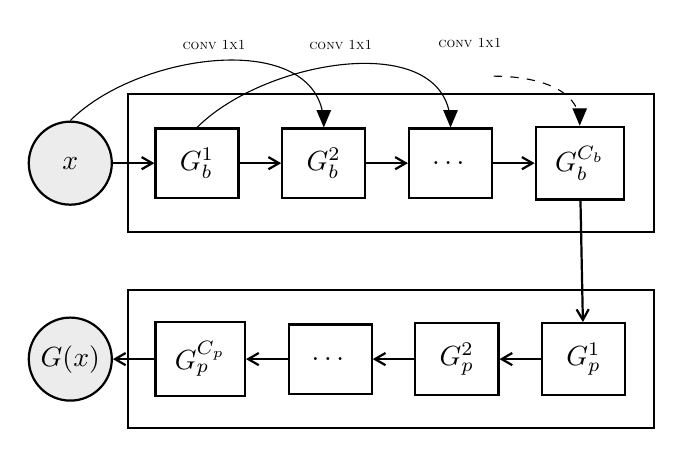
\begin{tikzpicture}
\node[io] (x) {$x$};
\node[group, minimum height=2.5em, minimum width=3em, right=1.5em of x] (b1) {$G_b^1$};
\node[group, minimum height = 5em, minimum width = 19em, right = 0.5em of x] (basestack) {};
\node[group, minimum height=2.5em, minimum width=3em, right=1.5em of b1] (b2) {$G_b^2$};
\node[group, minimum height=2.5em, minimum width=3em, right=1.5em of b2] (bdots) {\dots};
\node[above=1.5em of bdots] (invi2) {};
\node[right=0.5em of invi2] (invi) {};
\node[group, minimum height=2.5em, minimum width=3em, right=1.5em of bdots] (bc) {$G_b^{C_b}$};
\node[io, below=4em of x] (psix) {$G(x)$};
\node[group, minimum height = 5em, minimum width = 19em, right = 0.5em of psix] (specstack) {};
\node[group, minimum height=2.5em, minimum width=3em, right=1.5em of psix] (pc) {$G_p^{C_p}$};
\node[group, minimum height=2.5em, minimum width=3em, right=1.5em of pc] (pdots) {\dots};
\node[group, minimum height=2.5em, minimum width=3em, right=1.5em of pdots] (p2) {$G_p^{2}$};
\node[group, minimum height=2.5em, minimum width=3em, right=1.5em of p2] (p1) {$G_p^{1}$};
%\node[group2, minimum height=4.5em, minimum width=20em, right=1.1em of x] (bstack) {};
%\node[group2, minimum height=4.5em, minimum width=20em, right=1.1em of psix] (pstack) {};
\draw[conn] (x)--(b1);
\draw[conn] (b1)--(b2);
\draw[conn] (b2)--(bdots);
\draw[conn] (bdots)--(bc);
\draw[->] (x.north) to [out=45,in=90] (b2.north) node[above left=3.5em]{\tiny{\textsc{conv 1x1}}};
\draw[->] (b1.north) to [out=45,in=90] (bdots.north) node[above left=3.5em]{\tiny{\textsc{conv 1x1}}};
\draw[dashed,->] (invi.east) to [out=0,in=90] (bc.north) node[above left=3.5em]{\tiny{\textsc{conv 1x1}}};
\draw[conn] (bc)--(p1);
\draw[conn] (p1)--(p2);
\draw[conn] (p2)--(pdots);
\draw[conn] (pdots)--(pc);
\draw[conn] (pc)--(psix);
\end{tikzpicture}
\caption{Feature mapping induced by the component stacks of our architecture space. Each cell in the base stack receives outputs from two previous cells, whereas each cell in the personalized stack receives outputs from only one previous cell.}
\label{app-nas-fig:architecture}
\end{figure}

\noindent Generally, we assume that the tasks are broadly related and diverge in finer details. Therefore, the base architecture stack is designed to be significantly more expressive than the personalized stack, via employing a larger operator vocabulary and a more sophisticated propagation scheme as shown in Fig.~\ref{c4-fig:architecture}. In addition, as we will subsequently discuss in Section~\ref{c4-subsec:objective}, our objective is formulated such that its gradient evaluation will require approximating the Hessian of the personalized component. As such, a minimally expressive personalized stack is also a practical design to lower the computational cost. 


\subsection{Personalized Federated Learning Objective}
\label{c4-subsec:objective}
In this section, we will now discuss the learning objective of \textsc{FedPNAS}, which enables the discovery of personalized architecture. Let $\theta = \{\theta_b, \theta_p\}$ respectively denote all trainable parameters of the two component stacks above. In particular, $\theta_b=\{W_b, \Pi_b\}$ contains the concatenated weights $W_b$ of all edge operators; and the concatenated parameters $\Pi_b = [\Pi^t_e]_{t\in [C_b], e\in E_t}$ of the joint edge sampling distribution. Likewise, $\theta_p=\{W_p, \Pi_p\}$ contains their counterparts in the personalized stack. Given $N$ local clients with tasks $\{\Omega_1, \Omega_2 \dots \Omega_N\}$, the straight-forward extension of FL objective to the NAS problem defined by this search space can be written as:
\begin{eqnarray}
\theta_{\ast} &=& \underset{\theta}{\mathrm{argmax}} \frac{1}{N} \sum_{i=1}^N F_{\Omega_i}(\theta)
\label{c4-eq:flobj}
\end{eqnarray}
\citet{McMahan17} proposes a privacy preserving approach to optimize this objective by alternating between two communication steps of the model parameters. At any iteration $t \geq 0$:
\begin{itemize}
    \item Each local client performs a local gradient step with its current parameter $\theta^{t}_i$ and sends the suggested update $\bar{\theta}^t_i = \theta^t_i + \lambda\nabla_{\theta} F_{\Omega_i}(\theta^t_i)$ to a central server.
    \item The central server then computes $\theta^{t}_{\textsc{server}} = \frac{1}{N}\sum_{i=1}^N \bar{\theta}^t_i$ and broadcasts the aggregated parameters $\theta^{t}_{\textsc{server}}$ to all clients.
    \item Each local client performs the update $\theta^{t+1}_i \leftarrow \theta^{t}_{\textsc{server}}$ and prepares for the $(t+1)^{\text{th}}$ communication round.
\end{itemize}
This FL scheme implies that all clients will follow the same architecture distribution after the last communication round, which is not necessarily optimal in a heterogeneous task setting. To address this, our framework instead adopts the MAML meta learning objective~\citep{Finn17}, which aims to find a favorable initialization of $\theta$ that yields maximum averaged performance \textit{given an expected adaptation step}. This is different from Eq.~\ref{c4-eq:flobj}, which does not directly optimize for this initialization, but approximates it using the instantaneous averaged performance. Explicitly, this is achieved by the following objective:
\begin{eqnarray}
\theta_\ast &=& \underset{\theta_b, \theta_p}{\argmax} \frac{1}{N} \sum_{i=1}^N F_{\Omega_i}\left(\theta_b, \theta_p + \textcolor{red}{\lambda \nabla_{\theta_p} F_{\Omega_i}(\theta_b, \theta_p)} \right) \ ,
\label{c4-eq:fedpnasobj}
\end{eqnarray}
in which the difference from Eq.~\eqref{c4-eq:flobj}, highlighted in red, models a gradient ascent update with step size $\lambda$ to the aggregated personalized parameters $\theta_p$, which is to be conducted by each client at the end of the federated phase. Intuitively, this gradient step acts as a regularization term which favors $\theta$ that are simultaneously close to all task-specific optima and yield the best averaged performance after the adaptation phase. 

We now derive the gradient of this objective and discuss a practical algorithm to perform its computation. First, we let $\tilde{\theta}^t \triangleq \left(\theta^t_b, \theta^t_p + \lambda \nabla_{{\theta}^t_p} F_{\Omega}(\theta^t_b, \theta^t_p)\right)$ denote the anticipated update of $\theta$ at time $t$ of some arbitrary client. Then, dropping the client index for clarity, we subsequently derive the gradient ascent update for each client pertaining to the above personalized FL objective:
\begin{eqnarray}
\bar{\theta}^t &=& \theta^t + \lambda \nabla_{\theta^t} F_{\Omega}\left(\tilde{\theta}^t\right)\nonumber \\
&=& \theta^t + \left(\lambda \nabla_{\theta^t}\tilde{\theta}^t \right)\left(\nabla_{\tilde \theta^t} F_{\Omega}(\tilde{\theta_t})\right) \nonumber \\
&=& \theta^t +
\left[
\begin{array}{cc}
     \lambda\mathbf{I} &  \lambda^2 \nabla_{\theta_b^t} \nabla_{\theta_p^t} F_{\Omega}(\theta^t_b, \theta^t_p)\\
     \mathbf{0} & \lambda^2 \nabla^2_{\theta_p^t} F_{\Omega}(\theta^t_b, \theta^t_p)
\end{array}
\right]
\left(\nabla_{\tilde \theta^t} F_{\Omega}(\tilde{\theta}^t)\right) \ ,
\label{c4-eq:fedpnasexactgrad}
\end{eqnarray}
where we applied chain rule in the second equality and subsequently expanded $\lambda \nabla_{\theta^t}\tilde{\theta}^t$ in the third equality. The second-order gradient terms $\nabla_{\theta_b^t} \nabla_{\theta_p^t} F_{\Omega}(\theta^t_b, \theta^t_p)$ and $\nabla^2_{\theta_p^t} F_{\Omega}(\theta^t_b, \theta^t_p)$, however, are expensive to evaluate exactly. In order to derive practical computations of these terms, we note that the first-order Taylor approximation of the Hessian $\nabla^2_{\theta_p^t} F_{\Omega}(\theta^t_b, \theta^t_p)$ can be written as:
\begin{eqnarray}
\hspace{-8mm}
\nabla^2_{\theta^t} F_{\Omega}(\theta^t_b, \theta^t_p) &=& 
\left[
\begin{array}{cc}
     \nabla^2_{\theta_b^t} F_{\Omega}(\theta^t_b, \theta^t_p) &   \nabla_{\theta_b^t} \nabla_{\theta_p^t} F_{\Omega}(\theta^t_b, \theta^t_p)\\
     \nabla_{\theta_p^t} \nabla_{\theta_b^t} F_{\Omega}(\theta^t_b, \theta^t_p) & \nabla^2_{\theta_p^t} F_{\Omega}(\theta^t_b, \theta^t_p)
\end{array}
\right] \nonumber \\
&\simeq&
\left[
\begin{array}{c}
     \nabla_{\theta_b^t} F_{\Omega}(\theta^t_b, \theta^t_p) \\  \nabla_{\theta_p^t} F_{\Omega}(\theta^t_b, \theta^t_p)
\end{array}
\right]
\left[
\begin{array}{c}
     \nabla_{\theta_b^t} F_{\Omega}(\theta^t_b, \theta^t_p) \\  \nabla_{\theta_p^t} F_{\Omega}(\theta^t_b, \theta^t_p)
\end{array}
\right]^\top \nonumber \\
&=& 
\left[
\begin{array}{cc}
     \nabla_{\theta^t_b} F_{\Omega}(\theta^t_b, \theta^t_p)\nabla^\top_{\theta^t_b} F_{\Omega}(\theta^t_b, \theta^t_p)&   \nabla_{\theta^t_b} F_{\Omega}(\theta^t_b, \theta^t_p)\nabla^\top_{\theta^t_p} F_{\Omega}(\theta^t_b, \theta^t_p)\\
     \nabla_{\theta^t_p} F_{\Omega}(\theta^t_b, \theta^t_p)\nabla^\top_{\theta^t_b} F_{\Omega}(\theta^t_b, \theta^t_p)& \nabla_{\theta^t_p} F_{\Omega}(\theta^t_b, \theta^t_p)\nabla^\top_{\theta^t_p} F_{\Omega}(\theta^t_b, \theta^t_p)
\end{array}
\right] \ .
\end{eqnarray}
Matching appropriate terms in the above derivation then implies the following approximations, which can be computed with a single forward-backward pass of the architecture:
\begin{eqnarray}
\nabla_{\theta_b^t} \nabla_{\theta_p^t} F_{\Omega}(\theta^t_b, \theta^t_p)
&\simeq& \nabla_{\theta^t_b} F_{\Omega}(\theta^t_b, \theta^t_p)\nabla^\top_{\theta^t_p} F_{\Omega}(\theta^t_b, \theta^t_p) \ ,
\\
\nabla^2_{\theta_p^t} F_{\Omega}(\theta^t_b, \theta^t_p) &\simeq& \nabla_{\theta^t_p} F_{\Omega}(\theta^t_b, \theta^t_p)\nabla^\top_{\theta^t_p} F_{\Omega}(\theta^t_b, \theta^t_p) \ .
\end{eqnarray}
Plugging this back to Eq.~\eqref{c4-eq:fedpnasexactgrad} gives:
\begin{eqnarray}
\bar{\theta}^t &\simeq& 
\theta^t + 
\left[
\begin{array}{cc}
     \lambda \mathbf{I} & \lambda^2 \nabla_{\theta^t_b} F_{\Omega}(\theta^t_b, \theta^t_p)\nabla^\top_{\theta^t_p} F_{\Omega}(\theta^t_b, \theta^t_p) \\
     \mathbf{0} & \lambda^2
     \nabla_{\theta^t_p} F_{\Omega}(\theta^t_b, \theta^t_p)\nabla^\top_{\theta^t_p} F_{\Omega}(\theta^t_b, \theta^t_p)
\end{array}
\right]
\left(\nabla_{\tilde \theta^t} F_{\Omega}(\tilde{\theta^t})\right) \ ,
\label{c4-eq:fedpnasapproxgrad}
\end{eqnarray}
where the term $\nabla_{\tilde \theta^t} F_{\Omega}(\tilde{\theta^t})$ requires another forward-backward pass to compute (i.e., $\tilde{\theta}^t$ is computed in the same pass with the two approximated gradient terms above). Overall, this results in a local update scheme which uses two forward-backward passes of the architecture per iteration:
\begin{itemize}
    \item Compute $F_{\Omega}(\theta^t)$ in the first forward pass.
    \item Perform backpropagation to obtain $\nabla_{\theta^t} F_{\Omega}(\theta^t) = \left[\nabla_{\theta^t_b} F_{\Omega}(\theta^t_b,\theta^t_p), \nabla_{\theta^t_p} F_{\Omega}(\theta^t_b,\theta^t_p)\right]$. 
    \item Compute  $\nabla_{\theta^t_b} F_{\Omega}(\theta^t_b, \theta^t_p)\nabla^\top_{\theta^t_p} F_{\Omega}(\theta^t_b, \theta^t_p)$ and  $\nabla_{\theta^t_p} F_{\Omega}(\theta^t_b, \theta^t_p)\nabla^\top_{\theta^t_p} F_{\Omega}(\theta^t_b, \theta^t_p)$.
    \item Compute $\tilde{\theta}^t = \left(\theta^t_b, \theta^t_p + \lambda \nabla^\top_{\theta^t_p} F_{\Omega}(\theta^t_b, \theta^t_p)\right)$.
    \item Compute $F_{\Omega}(\tilde{\theta}^t)$ in the second forward pass.
    \item Perform backpropagation to obtain $\nabla_{\tilde{\theta}^t} F_{\Omega}(\tilde{\theta}^t)$.
    \item Compute the update in Eq.~\eqref{c4-eq:fedpnasapproxgrad}.
\end{itemize}

\subsection{Context-Aware Operator Sampling}
\label{c4-subsec:opsampler}
Finally, this section describes the parameterization of the joint operator sampling distribution over the edges of $\mathcal{G}_O$. Let $O_G \triangleq \cup_{t\in[C]} O_{G_t}$ be the set of all selected edge operators in a distilled architecture $G$, where $O_{G_t} \triangleq \{o^t_e \in \mathcal{O}\}_{e\in E_t}$ in turn denotes the set of all selected edge operators in cell $G_t$ (i.e., in a single stack architecture).~\citet{hu2020} then assumes a fully factorizable sampling distribution:
\begin{eqnarray}
p(O_G) 
&=& \prod_{t\in[C]} p(O_{G_t}) 
\ = \ \prod_{t\in[C]} \prod_{e \in E_t} p^t_e(o^t_e; \Pi^t_e) \ , 
\end{eqnarray}
where $\Pi^t_e$ denotes the learnable parameters of the edge sampling distribution $p^t_e$ for every $t \in [C]$ and $e \in E_t$. This formulation, however, does not factor in the important context information carried by the input instance $\mathbf{x}$ and its subsequent embeddings as $\mathbf{x}$ propagates through $G$. While this approach might be sufficient when only one architecture needs to be distilled from $\mathcal{G_O}$, it is challenging to extend to the \emph{horizontal} NAS setting because every edge in the over-parameterized architecture $\mathcal{G_O}$ is required to maintain and optimize its own set of categorical distribution parameters. In the context of our \emph{horizontal} NAS problem, this means that the set of parameters that need to be personalized will also scale with the size of the architecture, hence posing both a computational and a convergence problem. 

To overcome this issue, we will instead look at the conditional sampling distribution $p(O_g \mid \mathbf{x})$ and subsequently model architecture distillation as a Markov chain decision process, where each cell in the architecture stack will sequentially determine its edge operators given the input feature it receives from previous cells. For simplicity, we give our factorization of $p(O_G \mid \mathbf{x})$ below as if the architecture contains a single stack of cells and uses a linear propagation scheme, but it would be trivial to extend this formulation to any other propagation scheme:
\begin{eqnarray}
p(O_G \mid \mathbf{x}) &=& p(O_{G_1} \mid \mathbf{x}) \prod_{t=2}^C p(O_{G_t} \mid O_{G_{t-1}}, \mathbf{x}) \nonumber \\
%&\simeq& \prod_{t=1}^C p\left(O_{G_t} \mid z_{v^t_0}\right) \nonumber \\
&\simeq& \prod_{t=1}^C \prod_{e\equiv(v,v')}^{e \in E_t} p^t_e\left(o^t_{v,v'} \mid z_{v}\right) 
\end{eqnarray}
where $z_{v}$ denotes the feature vector at an arbitrary node $v$ in $G$ and in the factorization above, we have also assumed that $z_{v}$ acts as the sufficient statistics of the random variable $o^t_{v,v'}$.

The advantage of this formulation is two-fold. First, it provides a natural mechanism to incorporate context information into the edge selection process, thus allowing $\textsc{FedPNAS}$ to efficiently memorize architecture distillation patterns across clients. Second, the above factorization of $p(O_G \mid \mathbf {x})$ as a product of edge-wise conditional probabilities further reveals a compact representation of all sampling parameters using a single neural network $\psi$, which reduces the number of parameters that require fine-tuning in the local adaptation phase. That is, for any edge $e \equiv (v, v') \in E_t$, its context-aware operator distribution conditioned on $z_v$ is given as $p^t_e(o^t_{v,v'} \mid z_{v}) \triangleq \mathrm{Cat}\left(D, \psi\left(z_{v}\right)\right)$, where $D$ denotes the number of operators in $\mathcal{O}$ and the neural network $\psi$ maps the $z_{v}$ to the event probabilities of a categorical distribution.

\section{Experiments}
\label{c4-sec:exp}
This section describes our experiments to showcase the performance of $\textsc{FedPNAS}$ compared to other NAS and FL benchmarks. Our empirical studies are conducted on two image recognition datasets: (a) the CIFAR-10 dataset~\citep{cifar10} which aims to predict image labels from $10$ classes given a train/test set of $50000/10000$ colour images of dimension $32 \times 32$ pixels; and (b) the MNIST dataset~\citep{lecun2010mnist} which aims to predict handwritten digits (i.e. $0$ to $9$) given a train/test set of $60000/10000$ grayscale images of dimension $28 \times 28$ pixels. Our search space entails $2^{40}$ possible architectures, which is detailed in Appendix D. We compare two variants of our framework, \textsc{CA-FedPNAS} (with context-aware operation sampler) and \textsc{FedPNAS} (without the operation sampler), against:
(a) \textsc{FedAveraging} of a fixed architecture to justify the need for NAS in FL; (b) \textsc{FedDSNAS} - which trivially extends DSNAS to the FL setting (Eq.~\eqref{c4-eq:flobj}); and finally (c) \textsc{CA-FedDSNAS}, which extends \textsc{FedDSNAS} with our context-aware sampler.

\subsection{Heterogeneous predictive tasks} 
We first design a control experiment to test our framework on heterogeneous tasks and demonstrate the necessity of architecture personalization. To simulate this scenario, we first distribute the data i.i.d across clients (10000/2000 and 12000/2000 training/test images per client for CIFAR-10 and MNIST datasets respectively). Then, we independently apply a different transformation to each partitioned dataset. Input images within the same train/test set is subject to the same transformation. In both our experiments, the client datasets are subjected to rotations of $-30^{\circ}, -15^{\circ}, 0^{\circ}, 15^{\circ}$ and $30^{\circ}$ respectively. Fig.~\ref{fig4} below shows the performance of all the methods in comparison, plotted against number of search epochs and averaged over the above rotated variants of CIFAR-10 and MNIST datasets.

\begin{figure}[h]
\begin{tabular}{ccc}
\hspace{-6mm}
\includegraphics[width=0.33\columnwidth]{nas_plots/exp4.png} & 
\hspace{-6mm}
\includegraphics[width=0.33\columnwidth]{nas_plots/exp3.png} & 
\hspace{-6mm}
\includegraphics[width=0.33\columnwidth]{nas_plots/exp8.png} \\
\hspace{-6mm} (a) & 
\hspace{-6mm} (b) & 
\hspace{-6mm} (c)
\end{tabular}    
\caption{Plotting average classification accuracy of various methods against no. training epochs on heterogeneous tasks derived from (a) MNIST and (b) CIFAR-10 dataset. Figure (c) compares cumulative running time of various methods against no. training epochs on the CIFAR-10 dataset.}
\label{fig4}
\end{figure} 
On the MNIST dataset (Fig.~\ref{fig4}b), all methods converge to a similar performance. Among the NAS benchmarks, \textsc{FedPNAS} and \textsc{FedDSNAS} both converge slower than \textsc{FedAvg} and start off with worse performance in early iterations. This is expected since \textsc{FedAvg} does not have to search for the architecture and it is likely that the default architecture is sufficient for the MNIST task. On the other hand, we observe that both \textsc{CA-FedPNAS} and \textsc{CA-FedDSNAS} converge much faster than their counterparts without the context-aware operation sampler component. This shows that making use of contextual information helps to quickly locate regions of high-performing architectures, especially on similar inputs.

On the CIFAR-10 dataset  (Fig.~\ref{fig4}a), we instead observe significant gaps between the worst performing \textsc{FedAvg} and other NAS methods. This is likely because the default architecture does not have sufficient learning capability, which confirms the need for customizing solutions. Among the NAS benchmarks, we again observe that both \textsc{CA-FedPNAS} and \textsc{CA-FedDSNAS} outperform their counterparts without our operation sampler, which confirms the intuition above. Most remarkably, our proposed framework \textsc{CA-FedPNAS} achieves the best performance (0.8) and significantly outperformed both variants of federated \textsc{DSNAS} (0.71 for \textsc{CA-FedDSNAS} and 0.63 for \textsc{FedDSNAS}). 

Lastly, Fig.~\ref{fig4}c shows the runtime comparison between three methods on the CIFAR-10 experiment. In terms of sampling time, we observe that there is negligible overhead incurred by using our context-aware sampler (\textsc{CA-FedDSNAS} vs. \textsc{FedDSNAS}). 
The time incurred by our update (\textsc{CA-FedPNAS}) scales by a constant factor compared to \textsc{CA-FedDSNAS} since we use exactly one extra forward-backward pass per update. 

\begin{table}
	\centering
	\begin{sc}
		\begin{tabular}{|c|c|c|c|}
		\hline
		\multirow{2}{*}{Heterogeneity} & Task & \multirow{2}{*}{FedDSNAS} &  \multirow{2}{*}{CA-FedPNAS}\\
		& Description & & \\
		\hline
		\multirow{5}{*}{Low} & Rotate -30 & 0.947 & \textbf{0.978} \\
		\cline{2-4}
		& Rotate -15 & 0.973 & \textbf{0.976} \\
		\cline{2-4}
		& Vanilla & \textbf{0.988} & 0.985 \\
		\cline{2-4}
		& Rotate 15 & 0.986 & \textbf{0.987} \\
		\cline{2-4}
		& Rotate 30 & 0.972 & \textbf{0.981} \\
		\hline
		\multirow{5}{*}{High} & HueJitter -0.5 & 0.966 & \textbf{0.978} \\
		\cline{2-4}
		& HueJitter 0.5 & 0.967 & \textbf{0.972} \\
		\cline{2-4}
		& Vanilla & 0.988 & \textbf{0.989} \\
		\cline{2-4}
		& Rotate -90 & 0.892 & \textbf{0.932} \\
		\cline{2-4}
		& Rotate 90 & 0.866 & \textbf{0.932} \\
		\hline
	\end{tabular}
	\end{sc}
	\caption{Predictive accuracy of  \textsc{CA-FedPNAS} \textsc{FedDSNAS} on tasks with varying heterogeneity levels. \textsc{Rotate X}  denotes a rotation transformation of \textsc{X}$^{\circ}$ on client data; \textsc{Vanilla} denotes the original MNIST images; and \textsc{HueJitter X} denotes a hue jitter transformation of training images by a factor of \textsc{X}. The best performance in each row is in bold font.}
	\label{c4-table:1}
\end{table}

\subsection{Tasks with varying heterogeneity levels}
We expand the above study by subsequently investigating the respective performances of \textsc{CA-FedPNAS} and \textsc{FedDSNAS} on tasks with varying levels of heterogeneity. At low levels of heterogeneity, we deploy these methods on 5 sets of slightly rotated MNIST images. At high levels of heterogeneity, we employ a more diverse set of transformations on MNIST images, such as hue jitter and large angle rotations of $90^{\circ}$ and $-90^{\circ}$. Table~\ref{c4-table:1} shows the respective result of each task from these two settings. We observe that our method $\textsc{CA-FedPNAS}$ achieves better performance on most tasks and the performance gaps on tasks with higher heterogeneity are more pronounced (i.e., up to $7\%$ improvement on \textsc{Rotate 90} task). This clearly shows the importance of architecture personalization when the training tasks are significantly different and justifies our research goal.

\subsection{Knowledge transfer to completely new tasks} 
Finally, we conduct an ablation study to assess the quality of the \emph{pre-adaptation} architecture distributions respectively discovered by \textsc{CA-FedPNAS} and  \textsc{FedDSNAS}. In particular, we will leverage these learned distributions, which supposedly capture the broad commonalities of the task distribution, to generalize to completely unseen tasks (i.e., tasks that do not participate in the federated learning phase). To simulate this scenario, we train both methods on five clients whose local data consist of 12000 rotated CIFAR-10 images (i.e., in the range of $\pm 30^{\circ}$), similar to the setting of the first experiment. During the evaluation phase, however, we supply each local client with 2000 test images subjected to related but completely unseen transformations (i.e., $90^{\circ}$ and $-90^{\circ}$ rotations). 

\begin{table}[h]
	\centering
	\begin{sc}
		\begin{tabular}{|c|c|c|c|c|}
		\hline
		Unseen Task &  \multirow{2}{*}{FedDSNAS} & \multirow{2}{*}{CA-FedPNAS} & FedDSNAS & CA-FedPNAS \\
		Description & & & (Retrained) & (Retrained) \\
		\hline
		Rotate -90 & 0.545 $\pm$ 0.04 & 0.578 $\pm$ 0.09 & 0.699 $\pm$ 0.12 & \textbf{0.734 $\pm$ 0.17} \\
		\hline
		Rotate 90 & 0.553 $\pm$ 0.12 & 0.569 $\pm$ 0.06 & 0.673 $\pm$ 0.13 & \textbf{0.727 $\pm$ 0.22} \\
		\hline
		\end{tabular}
	\end{sc}
	\caption{Predictive accuracy (averaged over 5 clients) and standard deviation of \textsc{CA-FedPNAS} and \textsc{FedDSNAS} on two unseen tasks (CIFAR-10).}
	\label{c4-table:2}
\end{table}

\noindent We summarize our results in Table~\ref{c4-table:2} above. First, we measure the performance of \textsc{CA-FedPNAS} and \textsc{FedDSNAS} without any weight retraining. When received no additional information from the unseen tasks, both methods perform poorly as expected. While $\textsc{CA-FedPNAS}$ achieves better predictive accuracy, the performance gap in this scenario is negligible. To provide additional clues for adaptation, albeit minimal, we retrain the weights of each local model with 200  images that are rotated according to their respective unseen task description. With only 100 retraining iterations on limited data, \textsc{CA-FedPSNAS} already outperforms \textsc{FedDSNAS} (5\% and 8\% improvement respectively on two unseen tasks). This implies that \textsc{CA-FedPNAS} has captured more accurately the broad similarity of the task spectrum and requires minimal additional information to successfully adapt to unseen tasks.
\backmatter

%\renewcommand{\baselinestretch}{1.0}\normalsize

% By default \bibsection is \chapter*, but we really want this to show
% up in the table of contents and pdf bookmarks.
\renewcommand{\bibsection}{\chapter{\bibname}}
%\newcommand{\bibpreamble}{This text goes between the ``Bibliography''
%  header and the actual list of references}
\bibliographystyle{plainnat}
\bibliography{thesis} %your bib file

\end{document}
